\documentclass[11pt,]{article}
\usepackage{lmodern}
\usepackage{amssymb,amsmath}
\usepackage{ifxetex,ifluatex}
\usepackage{fixltx2e} % provides \textsubscript
\ifnum 0\ifxetex 1\fi\ifluatex 1\fi=0 % if pdftex
  \usepackage[T1]{fontenc}
  \usepackage[utf8]{inputenc}
\else % if luatex or xelatex
  \ifxetex
    \usepackage{mathspec}
  \else
    \usepackage{fontspec}
  \fi
  \defaultfontfeatures{Ligatures=TeX,Scale=MatchLowercase}
\fi
% use upquote if available, for straight quotes in verbatim environments
\IfFileExists{upquote.sty}{\usepackage{upquote}}{}
% use microtype if available
\IfFileExists{microtype.sty}{%
\usepackage{microtype}
\UseMicrotypeSet[protrusion]{basicmath} % disable protrusion for tt fonts
}{}
\usepackage[margin=1in]{geometry}
\usepackage{hyperref}
\PassOptionsToPackage{usenames,dvipsnames}{color} % color is loaded by hyperref
\hypersetup{unicode=true,
            pdftitle={Draft},
            colorlinks=true,
            linkcolor=Maroon,
            citecolor=Blue,
            urlcolor=blue,
            breaklinks=true}
\urlstyle{same}  % don't use monospace font for urls
\usepackage{longtable,booktabs}
\usepackage{graphicx,grffile}
\makeatletter
\def\maxwidth{\ifdim\Gin@nat@width>\linewidth\linewidth\else\Gin@nat@width\fi}
\def\maxheight{\ifdim\Gin@nat@height>\textheight\textheight\else\Gin@nat@height\fi}
\makeatother
% Scale images if necessary, so that they will not overflow the page
% margins by default, and it is still possible to overwrite the defaults
% using explicit options in \includegraphics[width, height, ...]{}
\setkeys{Gin}{width=\maxwidth,height=\maxheight,keepaspectratio}
\IfFileExists{parskip.sty}{%
\usepackage{parskip}
}{% else
\setlength{\parindent}{0pt}
\setlength{\parskip}{6pt plus 2pt minus 1pt}
}
\setlength{\emergencystretch}{3em}  % prevent overfull lines
\providecommand{\tightlist}{%
  \setlength{\itemsep}{0pt}\setlength{\parskip}{0pt}}
\setcounter{secnumdepth}{5}
% Redefines (sub)paragraphs to behave more like sections
\ifx\paragraph\undefined\else
\let\oldparagraph\paragraph
\renewcommand{\paragraph}[1]{\oldparagraph{#1}\mbox{}}
\fi
\ifx\subparagraph\undefined\else
\let\oldsubparagraph\subparagraph
\renewcommand{\subparagraph}[1]{\oldsubparagraph{#1}\mbox{}}
\fi

%%% Use protect on footnotes to avoid problems with footnotes in titles
\let\rmarkdownfootnote\footnote%
\def\footnote{\protect\rmarkdownfootnote}

%%% Change title format to be more compact
\usepackage{titling}

% Create subtitle command for use in maketitle
\newcommand{\subtitle}[1]{
  \posttitle{
    \begin{center}\large#1\end{center}
    }
}

\setlength{\droptitle}{-2em}
  \title{Draft}
  \pretitle{\vspace{\droptitle}\centering\huge}
  \posttitle{\par}
  \author{}
  \preauthor{}\postauthor{}
  \date{}
  \predate{}\postdate{}

\usepackage[retainorgcmds]{IEEEtrantools}
\usepackage{bm}
\usepackage{amsmath}
\usepackage{bbm}
\usepackage{hyperref}
\usepackage[lined,boxed]{algorithm2e}
\newtheorem{theorem}{Theorem}
\newtheorem{definition}{Definition}
\newtheorem{lemma}{Lemma}
\newtheorem{corollary}{Corollary}
\newcommand{\KL}{\,\text{KL}}
\newcommand{\der}{\,\text{d}}
\newcommand*{\Alignyesnumber}{\refstepcounter{equation}\tag{\theequation}}%

\begin{document}
\maketitle

{
\hypersetup{linkcolor=black}
\setcounter{tocdepth}{2}
\tableofcontents
}
\newpage

``In general, we look for a new law by the following process: First we
guess it. Then we -- now don't laugh, that's really true. Then we
compute the consequences of the guess to see what, if this is right, if
this law that we guessed is right, to see what it would imply. And then
we compare the computation results to nature, or we say compare to
experiment or experience, compare it directly with observations to see
if it works. If it disagrees with experiment, it's wrong. In that simple
statement is the key to science. It doesn't make any difference how
beautiful your guess is, it doesn't make any difference how smart you
are, who made the guess, or what his name is. If it disagrees with
experiment, it's wrong. That's all there is to it.''

\begin{itemize}
\tightlist
\item
  Richard Feynman in \emph{Richard Feynman Messenger Lectures at Cornell
  University: The Character of Physical Law. Chapter 7, Seeking New
  Laws}.
\end{itemize}

\newpage

\section{Abbreviations}\label{abbreviations}

Kullback-Leibler divergence between distributions \(\nu_i\) and
\(\nu_j\): \(\KL(\nu_i||\nu_j)\).

Binary relative entropy:
\(d(x,y) := x \log(x/y) + (1-x) \log((1-x)/(1-y))\), where
\(d(0,0) = d(1,1) = 0\).

Kullback-Leibler divergence for two Bernoulli distributions
parameterized by their means \(\mu_i\) and \(\mu_j\):
\(KL_{Ber}(\nu_i||\nu_j) = d(\mu_i, \mu_j)\).

\newpage

\section{\texorpdfstring{Introduction
\label{chap:Introduction}}{Introduction }}\label{introduction}

The thesis at hand joins the ranks of a large literature concerned with
the general problem of sequential sampling. One is familiar with the
idea of ``batch sampling'', where the entire sample is gathered first
and analyzed only after the last sample has become available. However,
as noted in Chernoff (1958), many situations arise in which one would
like to gather feedback from samples as they are drawn so as to
influence the choice of the next sample. The two fundamental
characteristics of the latter sampling process are that it is sequential
and adaptive. Since observations are drawn in sequence, one has a chance
to observe the observations drawn so far in order to adapt the decision
of what sample one would like to observe next.

This makes sequential sampling especially relevant in situations where
there is a inherent cost to drawing an observation. The classical
example that of clinical trials in which a researcher tests two drugs on
patients to observe which one performs better. Not only is it difficult
to gather patients, but also one would like to adapt the sampling such
that as soon as possible more patients receive the better drug so that
more patients are cured. As noted in Cappé et al. (2013), this example
dates back to Thompson (1933, 1935). Such problems are known as
multi-armed bandit problems in which the sampling is adapted so as to
minimize the cumulative regret: In the case of the drug tests, one would
like to sample the two drugs in a way to find the best drug as soon as
possible and then to test this drug more and more often and more often
than the worse drug. This would lead to cumulatively more healthy
patients then when both drugs are tested uniformly and thus minimize the
regret from treating a patient with an ineffective drug.

Instead of drugs, can consider two or more unknown distributions (which
we call arms in the multi-armed bandit problem). These distributions
have different means, and one can draw samples sequentially from the
distributions in order to estimate their means. One would like to play
the distribution with the highest mean to minimize the cumulative regret
measure. How can we organize the sampling in order to achieve this goal?

While Gittins (1979) presents an Bayesian-optimal solution, the
Upper-Confidence Bound algorithms pioneered by Agrawal (1995) and Auer,
Cesa-Bianchi and Fischer (2002) lead to a blooming literature on
multi-armed bandit problems that has been picked up to solve modern
problems in website and advertising optimization, where advertisers try
to allocate their advertising optimally so as to reduce regret from
showing poorly converting advertisements. Several algorithms as the
KL-UCB algorithm based on Kullback-Leibler divergence upper confidence
intervals (Cappé et al., 2013) or the Bayes-UCB algorithm (Kaufmann et
al., 2012) have followed and been shown to be optimal as they reach the
lower bound introduced in Lai and Robbins (1985) and Burnetas and
Katehakis (1996).

These algorithms have in common that they compute after any sample an
index for each of the unknown distributions. This index is based solely
on the past (observed) data, and then used to pick the distribution from
which the next observation should be drawn. Using these indexes, the
algorithms can sequentially sample and adapt the future strategies to
observations as they are gathered.

Other algorithms based on indices can be used on related problems.
Instead of minimizing cumulative regret, it might be more interesting to
find the best arm, that is, the distribution with the largest mean, with
as few samples as possible and with confidence as large as possible.
This is particularly useful when there is not necessarily a cost from
initially picking a lower mean, but when drawing any sample is costly,
and one needs to explore the distributions as efficiently as possible.
The need for strategies other than uniform sampling arises: Do not
continue to sample distributions that we are confident about. As such,
the best arm identification problem is very similar to the problem faced
in Bayesian Optimization: Training large neural networks is costly in
terms of time and computation, and so the parameter space needs to be
explored with as few samples as possible. (Zhang et al., 2017; Brochu et
al., 2010).

The problem of best arm identification is very related to statistical
hypothesis testing as noted by Chernoff (1958) since in the end, one has
to make a decision about how the means of distributions relate to each
other. The main difference of course being that the sampling procedure
becomes integrated into the evaluation of the distributions. Given the
focus on exploration, the problem is usually described with a loss
function different from cumulative regret. Audibert et al. (2010)
introduce a soft measure called \emph{simple regret} based on which they
describe UCB policies. Other authors investigate hard, binary measures
that are equal to 1 when the best arm has not been identified (Russo,
2016; Garivier and Kaufmann, 2016). These binary measures correspond to
the probability of the identified arm being the best, and thus
inherently related to hypothesis testing. The problem of best arm
identification can readily be extended to the so called Top-\(m\)
problem of identifying the best \(m\) of \(K\) arms (Kaufmann and
Kalyanakrishnan, 2013; Kaufmann et al. 2016).

In this thesis, we consider the thresholding bandit problem. Instead of
identifying the best \(m\) out of \(K\) arms, one aims to find all out
of \(K\) distributions that have a mean larger than a threshold fixed
upfront. In the form described in Locatelli et al. (2016), algorithms in
the thresholding bandit problem are evaluated against a binary loss
function penalizing whenever an arm has not been classified correctly as
being above the threshold and thus focus on exploration similar to
algorithms employed for best arm identification. Indeed, Locatelli et
al. (2016) show how their thresholding algorithm can be used for best
arm identification when the mean of the best arm is known upfront.

In the following, we first present the thresholding bandit problem in
detail. To then extend upon the algorithm proposed by Locatelli et al.
(2016), we first explore how the Kullback-Leibler divergence has been
employed in the best arm identification literature by Garivier and
Kaufmann (2016) and Kaufmann et al. (2016). We shortly describe two
variance based algorithms for the thresholding bandit problem introduced
in Mukherjee et al. (2017) and Zhang et al. (2017), before introducing
the new Simple Likelihood Ratio algorithm. We end with experiments to
examine the performance of different algorithms.

\newpage

\section{\texorpdfstring{The Thresholding Bandit Problem
\label{chap:ThresholdingBanditProblem}}{The Thresholding Bandit Problem }}\label{the-thresholding-bandit-problem}

To introduce the thresholding bandit problem, consider a game in which
the learner is tasked to find those slot machines within a row of \(K\)
slot machines in a casino that give a mean payoff larger than a fixed
threshold \(\tau\), for example \(\tau = 0\). The learner cannot pull
all slot machines at the same time. Instead, he acquires samples
sequentially from one slot machine at a time to learn about their payoff
structure. The learner has a budget of \(T\) slot machine pulls. After
\(t-1\) samples, the learner has observed \(T_i(t-1)\) samples from slot
machine \(i\). The payoffs \(X_{i,1}, ..., X_{i,T_i(t-1)}\) are drawn
from the payoff distribution \(\nu_i\) underlying the slot machine
\(i\). At time \(t\), the learner considers the payoffs he observed so
far in order to choose the next slot machine he would like to pull. His
decision is lead by the goal to classify the slot machines with
distribution \(\nu_i\) and mean payoff
\(\mu_i = \mathbb{E}_{X \sim \nu_i}[X]\) after \(T\) samples as being
above or below the threshold with error probability as small as
possible.

The thresholding bandit problem can thus be framed in the wide
literature on sequential sampling strategies. While its name is
reminiscient of the multi-armed bandit setting, the thresholding bandit
problem is more akin to best arm identification and Top-\(m\)
identification problems due to its focus on exploration: While the
classical multi-armed bandit problems are concerned with cumulative
regret which increases \emph{during} sampling, best arm identification
and thresholding bandits collect loss only once \emph{after} the
sampling procedure (compare Garivier and Kaufmann, 2016; Kaufmann et
al., 2016; Kaufmann and Kalyanakrishnan, 2013). Furthermore, as there
arises an implicit threshold between the means of the \(m\)-th best arm
and the \(m+1\)-th best arm (Kaufmann et al., 2016; Kaufmann and
Kalyanakrishnan, 2013), algorithms for the Top-\(m\) identification
problem classify arms at least implicitly as being above or below a
threshold. The two settings are thus very related.

\subsection{\texorpdfstring{Setup
\label{sec:Setup}}{Setup }}\label{setup}

Consider a setting with a set of \(\mathbb{A}=\{1, ..., K\}\) unknown
probability distributions \(\nu_i, i \in \mathbb{A}\). To stick with the
idea of multi-armed bandits, we call those distributions arms, and
observations from those arms rewards (Bubeck and Cesa-Bianchi, 2012).
The learner is interested in learning about the structure of the arms;
in particular, he would like to estimate the means \(\mu_1, ..., \mu_K\)
by sequentially drawing observations \(X_{i,1}, X_{i,2}, ...\) from each
arm. However, at time \(t\) the learner cannot observe a reward from
every distribution but must select a single arm \(I_t\) from which he
would like to observe the reward \(X_{I_t,t}\). An adaptive sampling
strategy makes the decision of which arm to pull usually by computing an
index \(B_i(t)\) for each arm. If \(T_i(t)\) is the number of samples
observed until time \(t\) for arm \(i\), then \(B_i(t)\) is a function
of the past rewards \(X_{i,1}, ..., X_{i,T_i(t)}\) observed for arm
\(i\), and w.l.o.g. \(I_t = \arg \min_{i = 1,...K} B_i(t)\). The set of
indices can be called strategy (Kaufmann et al., 2012) which makes it
clear that the strategy is adapted as more observations are collected.
Strategies of this kind are also called index policies.

What index proves to be useful is determined by the loss function with
which the decisions of the algorithm are evaluated. While many problems
are concerned with finding the arm with the largest mean \(\mu_i\), in
which algorithms collect loss either cumulatively (Auer and
Cesa-Bianchi, 2012) or once at the end of the sampling (Kaufmann et al.,
2016), the thresholding bandit problem considers a slightly different
loss function. Consider a fixed threshold value \(\tau \in \mathbb{R}\)
and an epsilon interval \(\tau \pm \epsilon\) around the threshold for
\(\epsilon \geq 0\). As mentioned in the introduction, the learner is
tasked with classifying arms as having a mean \(\mu_i\) larger or
smaller than \(\tau\). To describe which arms are above the threshold,
we introduce the following set notation (compare Locatelli et al.,
2016): Let \(\mathcal{S}_{\tau}\) be the set of distributions in
\(mathbb{A}\) with mean larger than the threshold:
\(\mathcal{S}_{\tau} := \{i \in \mathbb{A}, \mu_i \geq \tau\}\).
Consequently, the complement is given by the arms with mean below the
threshold,
\(\mathcal{S}^C_{\tau} := \{i \in \mathbb{A}, \mu_i < \tau\}\).

The thresholding problem for the learner is now to use a budget of
overall \(T\) samples (or rounds) to explore the different arms. After
this exploration phase, the learner has to return a set of arms that he
believes to have a mean above the threshold. The problem can thus be
described by the threshold \(\tau\) and a precision \(\epsilon\). When
evaluating the classification of the learner, arms with mean inside of
the epsilon interval will not be considered. The learner only has to
distinguish the means from the threshold correctly up to the precision
\(\epsilon\). Thus, the algorithm is not evaluated against
\(\mathcal{S}_{\tau}\) and \(\mathcal{S}^C_{\tau}\), but needs to
distinguish \(\mathcal{S}_{\tau+\epsilon}\) from
\(\mathcal{S}^C_{\tau-\epsilon}\). As in Locatelli et al. (2016),
whenever we say that ``an arm is over the threshold'', we mean that the
mean of the arm is over the threshold.

The learner's classification is returned as the set
\(\hat{\mathcal{S}}_{\tau} := \hat{\mathcal{S}}_{\tau}(T) \subset \mathbb{A}\)
after \(T\) rounds; that is, the set of arms estimated to be over the
threshold. The classification is evaluated against the loss given as
(Locatelli et al., 2016):

\[
\mathcal{L}(T) = \mathbbm{1}{(\hat{\mathcal{S}}_{\tau} \cap \mathcal{S}_{\tau-\epsilon}^C \neq \emptyset) \lor (\hat{\mathcal{S}}_{\tau}^C \cap \mathcal{S}_{\tau+\epsilon} \neq \emptyset)}
\]

In order to perform well, a learner has to identify all arms that are
over the threshold as such, and to not claim arms as being over the
threshold if they actually are below the threshold. Due to the precision
\(\epsilon\), the loss is not influenced by arms which are too close to
the threshold \(\tau\), that is, arms inside of the
\(\tau \pm \epsilon\) interval. If either \(\hat{\mathcal{S}}_{\tau}\)
contains an arm below \((\tau - \epsilon)\), or
\(\hat{\mathcal{S}}^C_{\tau}\) contains an arm above
\((\tau + \epsilon)\), a loss of \(1\) is accrued. Else, all arms
outside the epsilon interval are classified correctly and the loss is
equal to \(0\). In the case of \(\epsilon = 0\), all arms need to be
classified correctly to not endure any loss.

Algorithms for this thresholding problem can be compared based on their
expected loss. Let \(\mathbb{E}\) be the expectation with regard to the
samples \(X_{i,1}, ..., X_{i,T}\) collected by the algorithm. The
expected loss is then given as

\[
\mathbb{E}[\mathcal{L}(T)] = \mathbb{P}\big((\hat{\mathcal{S}}_{\tau} \cap \mathcal{S}_{\tau-\epsilon}^C \neq \emptyset) \lor(\hat{\mathcal{S}}_{\tau}^C \cap \mathcal{S}_{\tau+\epsilon} \neq \emptyset)\big),
\]

which corresponds to the probability of making a wrong classification.
Both the probability of not identifying an arm that is actually over the
threshold, as well as the probability of accepting an arm as over the
threshold when it is not are evaluated. The oracle strategy would
evaluate all arms correctly with an error probability of \(0\)
(Locatelli et al., 2016).

At this point, we have introduced the general thresholding bandit
problem setting which we will use throughout the thesis. The setting
might be extended by different assumptions to make certain algorithms or
bounds feasible. For that reason, Locatelli et al. (2016) assume that
the distributions \(\nu_i, i \in \mathbb{A}\) are \(R\)-sub-Gaussian.
Under this assumption, the authors are able to prove a lower bound on
the largest probability of error of the best algorithm in the setting we
have just introduced, as well as an upper bound on the performance of
their APT algorithm we will introduce in the following chapter. As in
their paper, we define \(R\)-sub-Gaussian and assume it in the
description of their algorithm and bounds:

\begin{definition}[$R$-sub-Gaussian distribution] 
\label{definition:rsubgaussian}
Let $R > 0$. A distribution $\nu$ is $R$-sub-Gaussian if for all $t \in \mathbb{R}$ we have
\begin{equation*}
\mathbb{E}_{X \sim \nu}[\exp(tX - t\mathbb{E}[X])] \leq \exp(R^2t^2/2).
\end{equation*}
\end{definition}

As noted by Locatelli et al. (2016), this ensures that the mean
\(\mu_i\) of the distributions \(\nu_i\) considered in our problem are
finite. \(R\)-sub-Gaussian distributions furthermore offer concentration
inequalities for the concentration of the empirical mean to the true
mean, which makes it possible to deduce the bounds presented by the
authors and repeated below. The family of \(R\)-sub-Gaussian
distributions encompasses Gaussian distributions of variance \(R^2\) for
\(R \in \mathbb{R}\), as well as all bounded distributions, with the
important case of Bernoulli distributions.

Having described the thresholding bandit setting as well as the
assumption of \(R\)-sub-Gaussianity, we can now proceed to describe the
\emph{Anytime Parameter-free Thresholding} (APT) algorithm proposed in
Locatelli et al. (2016) for the thresholding bandit problem.

\subsection{\texorpdfstring{The Anytime Parameter-free Thresholding
Algorithm
\label{sec:TheAPTAlgorithm}}{The Anytime Parameter-free Thresholding Algorithm }}\label{the-anytime-parameter-free-thresholding-algorithm}

In the following we describe the \emph{Anytime Parameter-free
Thresholding} (APT) algorithm proposed in Locatelli et al. (2016), which
is a simple yet effective algorithm and displays some very favorable
characteristics when compared to alternative algorithms.

We fix the threshold \(\tau\) and epsilon interval around the threshold
given by \(\epsilon\) upfront, and supply them as arguments to the
algorithm: \((\tau, \epsilon)\). Based on the general thresholding
problem, we demand that the algorithm draws samples \(X_{i,t}\) for
\(T\) rounds from the distributions \(\nu_i, i\in \mathbb{A}\). For a
given arm \(i\) and a given time \(t\), we let \(T_i(t)\) represent the
number of samples drawn from arm \(i\) until time \(t\) (including).
Consequently, the empirical mean of arm \(i\) at time \(t\) is given by
\(\hat{\mu}_i(t) = \frac{1}{T_i(t)} \sum_{s=1}^{T_i(t)} X_{i,s}\) where
\(X_{i,s}\) is the feedback sampled from distribution \(\nu_i\) when the
arm is pulled for the \(s\)-th time. In the case of the APT algorithm,
the decision \(\hat{\mathcal{S}}_{\tau}\) is based on the empirical
means \(\hat{\mu}_i(T)\) estimated from the samples drawn up to time
\(T\):
\(\hat{\mathcal{S}}_{\tau} := \hat{\mathcal{S}}_{\tau}(T) = \{i \in \mathbb{A}, \hat{\mu}_i(T) \geq \tau\}\).

As we see in algorithm \ref{alg:APT}, the APT algorithm initiates by
pulling each arm once. Then, for each \(t > K\), it calculates for every
arm the values \(T_i(t)\) and \(\hat{\mu}_i(t)\). Based on the empirical
mean, the algorithm computes the estimated gap between the mean and the
threshold as
\(\hat{\Delta}_i(t) = \hat{\Delta}_i^{\tau, \epsilon}(t) = |\mu_i(t) - \tau| + \epsilon\).
The decision of which arm is sampled next is then based on the value
\(B_i(t+1) = \sqrt{T_i(t)} \hat{\Delta}_i(t)\): the algorithm pulls arm
\(I_{t+1} = \arg \min_{i\leq K} B_i(t+1)\) minimizing this decision
quantity. After overall \(T\) pulls, the algorithm returns the sets
described in the general setup, \(\hat{\mathcal{S}}_{\tau}\) and
\(\hat{\mathcal{S}}^C_{\tau}\).

\IncMargin{1em}

\begin{algorithm}
\SetKwData{Left}{left}\SetKwData{This}{this}\SetKwData{Up}{up}
\SetKwFunction{Union}{Union}\SetKwFunction{FindCompress}{FindCompress}
\SetKwInOut{Input}{Input}\SetKwInOut{Output}{Output}
\Input{$\tau$, $\epsilon$}
\Output{$\hat{S}_{\tau} = \{k: \hat{\mu}_k(T) \geq \tau\}$}
\BlankLine
\emph{Pull each arm once}\;
\For{$t = K+1$ \KwTo $T$}{
  \emph{Pull arm $I_t = \arg \min_{k\leq K} B_k^{APT}(t) = \sqrt{T_k(t)} (|\hat{\mu}_i(t) - \tau|+\epsilon)$}\;
  \emph{Observe reward $X \sim \nu_{I_t}$}\;
}
\caption{Anytime Parameter-free Thresholding Algorithm (Locatelli et al., 2016)}\label{alg:APT}
\end{algorithm}

\DecMargin{1em}

Just like the general index policies mentioned in \autoref{sec:Setup},
we see that the APT algorithm adapts its strategy using an index
\(B_i(t+1)\) for each arm that is based entirely on the observations
observed until time \(t\). Given the arm with the smallest index is
pulled at round \(t+1\), we observe that arms that are estimated to be
further away from the threshold \(\tau\) as measured by the absolute
distance to their empirical mean \(\hat{\mu}_i\), \(\hat{\Delta}_i(t)\),
are pulled less often. Intuitively, it is easier to classify arms as
below or above \(\tau\) when their mean is far away from the threshold.
In contrast to the uniform sampling strategy, APT will gather more
evidence for arms which appear to be inherently more difficult to
classify. Likewise, APT tends to pull arms less often which it already
pulled considerably often as measured by \(T_i(t)\). If arm \(i\) has
been pulled more often than arm \(j\), then we should in general be more
confident in its estimated mean and the corresponding distance to the
threshold. If we are confident in \(i\), then it is better to explore
other arms by drawing an observation from arm \(j\). By adapting its
sampling strategy in this way during the sequential sampling process,
the APT algorithm minimizes the probability of error
\(\mathbb{E}[\mathcal{L}(T)]\) after \(T\) samples have been observed.

The previous paragraph describes how arms close to the threshold are
intuitively more difficult to classify. In the index employed by the APT
algorithm, the distance between an arm and the threshold is measured by
the absolute distance \(\hat{\Delta}_i(t)\) between the (estimated) mean
of the arm and the threshold \(\tau\) (and the epsilon interval). Given
that one compares \(B_i^{APT}\) with \(B_j^{APT}\), one could just as
well measure the distance by the squared distance,
\(\hat{\Delta}_i(t)^2\). When the APT algorithm realizes that an arm has
a mean close to the threshold, then this arm requires more attention
than an arm far away from the threshold; the confidence in the empirical
mean has to be larger. Or the empirical mean has to be better
concentrated around the true mean. Otherwise it is easier to make a
mistake on this arm. To gain this confidence, the arm requires more
samples, and thus a larger share of the overall \(T\) samples available.
With this intuition, it makes sense to measure the complexity of a
thresholding problem: If we knew upfront how complex a given set of arms
is, we knew whether we can expect a small or large probability of error
given our budget \(T\). Also, for example in the best arm identification
problem, there exist algorithms which take the complexity of a problem
as input. Based on the complexity they then adapt their sampling
strategy. See for example the UCB-E algorithm in Audibert et al. (2010)
for the best arm identification problem, or the KL-LUCB-E algorithm in
Kaufmann and Kalyanakrishnan (2013) as extension to the Top-\(m\)
problem.

While the APT algorithm does not require the complexity to be known
upfront (which would be problematic), it is necessary to define the
complexity to deduce the upper bound on its probability of error.
Similar to the distance measure used in the algorithm's index, we define
the gap \(\Delta_i^{\tau,\epsilon}\) between arm \(i\) and the threshold
\(\tau \pm \epsilon\) as

\[
\Delta_i := \Delta_i^{\tau,\epsilon} = |\mu_i - \tau| + \epsilon
\]

Given this gap, Locatelli et al. (2016) define the complexity
\(H_{\tau, \epsilon}\) for the thresholding bandit problem naturally as

\[
H := H_{\tau, \epsilon} = \sum_{i=1}^K \frac{1}{(\Delta_i^{\tau,\epsilon})^2}.
\]

Note that the complexity of the problem increases in the number of arms
\(K\) and decreases in the gap \(\Delta_i^{\tau,\epsilon}\).
Consequently, when we require a smaller precision, that is, we increase
\(\epsilon\), the hardness decreases. Furthermore, we see that each arm
contributes its individual complexity,
\(h_i^{\tau,\epsilon} = \frac{1}{(\Delta_i^{\tau,\epsilon})^2}\)
linearly into the problem. Thus, if the complexity \(H\) is a good
measure of the actual problem complexity, and we knew upfront which arm
has which mean, we could allocate the ``optimal'' share of the budget,
\(T \cdot h_i /H\) to arm \(i\). However, since we do not know neither
\(\mu_i\) nor \(H\), the best we can do is to adapt our allocation of
samples more and more towards this optimum as we observe samples.

At this point, one can question whether the measure of complexity \(H\)
proposed in Locatelli et al. (2016) is a good measure of the ``true''
problem complexity. In the following \autoref{sec:UpperBoundLocatelli},
we will show the upper bound on the probability of error for the APT
algorithm and see how the complexity \(H\) arises naturally for the APT
algorithm. In \autoref{sec:LowerBoundLocatelli} we then show the lower
bound presented in Locatelli et al. (2016) and that the APT algorithm is
optimal in that it matches the lower bound. We discuss the results and
the APT algorithm further in \autoref{sec:DiscussionLocatelli}.

\subsection{\texorpdfstring{Upper Bound for the APT Algorithm
\label{sec:UpperBoundLocatelli}}{Upper Bound for the APT Algorithm }}\label{upper-bound-for-the-apt-algorithm}

In this chapter we present the upper bound on the APT algorithm proven
in Locatelli et al. (2016). The upper bound is on the probability of
error that the algorithm has after \(T\) rounds of sampling for a
problem with arms that are assumed to be \(R\)-sub-Gaussian. The bound
depends also on the complexity of the problem, and we show in the proof
that given the index of the APT algorithm as defined in
\autoref{sec:TheAPTAlgorithm}, the complexity \(H\) is an appropriate
measure.

We now state the theorem as in Locatelli et al. (2016) and present a
proof.

\begin{theorem}[Theorem 2, Locatelli et al., 2016] \label{theorem:LocatelliTheorem4}
Let $K \geq 0$, $T \geq 2K$, and consider a problem $\mathcal{B}$. Assume that all arms $\nu_i$ of the problem are R-sub-Gaussian with means $\mu_i$. Let $\tau \in \mathbb{R}, \epsilon \geq 0$. Algorithm APT's expected loss is upper bounded on this problem as 
\begin{equation*} \mathbb{E}(\mathcal{L}(T)) \leq \exp
\Big(-\frac{1}{64R^2}\frac{T}{H} + 2 \log((\log(T) + 1)K)\Big) \end{equation*}

where we remind that $H = \sum_i (|\mu_i - \tau | + \epsilon)^{-2}$ and where
$\mathbb{E}$ is the expectation according to the samples of the problem.
\end{theorem}

\subsubsection{\texorpdfstring{Proof of Theorem
\ref{theorem:LocatelliTheorem4}}{Proof of Theorem }}\label{proof-of-theorem}

In order to upper bound the expected loss of the APT algorithm, we want
to define an event on which the algorithm correctly seperates arms from
the threshold, that is, a separation condition holds on this event. We
then want to show that this \emph{favorable} event does indeed hold with
large probability. Consequently, APT's probability of error will
correspond to the probability that the favorable event does not hold, as
this leads to a failure of the seperation condition, and consequently to
an incorrect classification of at least one arm by the algorithm. We
start by defining the separation condition.

\subsubsection{Separation Condition}\label{separation-condition}

As noted in Zhong et al. (2017), a simple requirement to correctly
classify arms at the final round is the following. For every arm
\(i \in \{1, ..., K\}\) after the final round \(T\), require \[
\hat{\mu}_{i,T_i(n)} \geq \mu_i - \frac{\mu_i - \tau + \epsilon}{2} \quad \text{if} \quad \mu_i \geq \tau
\] or \[
\hat{\mu}_{i,T_i(n)} \leq \mu_i + \frac{\tau - \mu_i + \epsilon}{2} \quad \text{if} \quad \mu_i < \tau
\] Or simply in terms of the gap between the arm and the threshold as
used in the index by the APT algorithm: \[
| \hat{\mu}_{i, T_i(n)} - \mu_i | \leq \frac{|\mu_i - \tau| + \epsilon}{2} = \frac{\Delta_i}{2}.
\]

Intuitively, this condition makes sense as it ensures that the current
mean estimate is closer to the true mean than to the threshold.
Consequently, there is no arrangement possible in which the arm is
classified wrong while the separation condition holds. Assuming
\(\mu_i < \tau\) and \(\epsilon = 0\), an incorrect classification would
require \(\mu_i < \tau \leq \hat{\mu_i}\). But then
\(| \hat{\mu}_{i, T_i(n)} - \mu_i | \geq |\mu_i - \tau|\), which
violates the separation condition.

Thus, we need to show that this condition holds for every arm
\(i \in \{1,...,K\}\) with large probability after the final round
\(T\). In different words, we need to derive an upper bound on the
probability with which this condition does not hold.

\subsubsection{The Favorable Event}\label{the-favorable-event}

The separation condition describes what event needs to hold in order for
the APT algorithm to make a correct classification: The smaller the
deviation of the empirical mean from the population mean, the more
difficult it is for the classification to be wrong. Moreover, if the
mean and empirical mean are identical, then the classification is
correct independent of the threshold. Also, the closer the mean to the
threshold, the better the estimate has to be for a correct
classification to be likely. To bound the absolute deviation of the
empirical mean from the true mean, we define the favorable event \(\xi\)
as

\[
\xi = \Big\{\forall i \in \mathbb{A}, \forall s \in \{1,...,T\} : |\frac{1}{s} \sum_{t=1}^{s}X_{i,t} - \mu_i| \leq \sqrt{\frac{T \delta^2}{H s}} \Big\}.
\]

The probability that this favorable event occurs should be large, or
equivalently, the probability that the deviation is small should be
large. Then it follows that the separation condition holds with large
probability.

We know that \(X_i\) are \(R\)-sub-Gaussian by assumption. That is, we
have

\[
\mathbb{E}[\exp (tX_{i,s}-t\mathbb{E}[X_{i,s}])] = \mathbb{E}[\exp (t(X_{i,s}-\mathbb{E}[X_{i,s}]))] \leq \exp (R^2t^2/2)
\]

where the RHS is the moment-generating function of the random variable
\(X_{i,s}-\mathbb{E}[X_{i,s}]\). While Höffding's Lemma and Höffding's
Inequality are commonly applied to bounded random variables \(Z\) with
\(\mathbb{P}(a\leq Z \leq b) = 1\) and \(\mathbb{E}[Z] = 0\), we see
that \(Z\) are \(R\)-sub-Gaussian with \(R^2 = \frac{(a-b)^2}{4}\).
Using this last equality, we can easily apply Höffding's Inequality to
our case.

\begin{lemma}[Höffding's Inequality (Kloft Lecture Notes)] \label{lemma:HoeffdingsInequality}
Let $X_1, ..., X_s$ be independent, identically distributed random variables with mean $\mathbb{E}[X_t] = \mu$ and $\mathbb{P}(a_t \leq X_t - \mathbb{E}[X] \leq b_t) = 1$. Denote their empirical mean by $\bar{X}_s=\frac{1}{s}\sum_{t=1}^{s}X_t$. Then, for any $\gamma > 0$, we have the following concentration inequality:

\begin{equation*}
\mathbb{P}(|\bar{X}_s - \mu| \geq \gamma) \leq 2\exp (-2s^2\gamma^2/\sum_{t=1}^s(b_t - a_t)^2).
\end{equation*}
\end{lemma}

If we replace \(\sum_{t=1}^s(b_t - a_t)^2\) by \(4sR^2\), we have the
concentration inequality for our \(R\)-sub-Gaussian random variables:

\[
\mathbb{P}(|\bar{X}_s - \mu| \geq \gamma) \leq 2\exp (-\frac{s\gamma^2}{2R^2}).
\]

Writing \(\gamma = \sqrt{\frac{T\delta^2}{Hs}}\), we get for the
favorable event
\(\xi_i = \{|\bar{X}_s - \mu| \leq \sqrt{\frac{T\delta^2}{Hs}}\}\) of an
individual arm \(i\), for each \(i \in \mathbb{A}\) and each
\(s \in \{1, ..., T\}\):

\[
\mathbb{P}(\xi_i) = \mathbb{P}\Big(|\bar{X}_{i,s} - \mu_i| \leq \sqrt{\frac{T\delta^2}{Hs}}\Big) \geq 1 - 2\exp (-\frac{T\delta^2}{2R^2H}),
\] where \(T\) is again the total budget of samples, and \(H\) the
complexity. Now let

\[
\tilde{\xi} = \Big\{\forall i \in \mathbb{A}: |\frac{1}{s} \sum_{t=1}^{s}X_{i,t} - \mu_i| \leq \sqrt{\frac{T \delta^2}{H s}} \Big\}.
\]

To derive the probability of event \(\tilde{\xi}\), we apply a union
bound on \(\mathbb{P}(\cup_{i=1}^K \xi_i^C)\):

\begin{align*}
\mathbb{P}(\tilde{\xi}) & = 1-\mathbb{P}(\xi^C) \\
& = 1-\mathbb{P}(\cup_{i=1}^K \xi_i^C) \\
& \geq 1 - \sum_{i=1}^K \mathbb{P}(\xi_i^C) \\
& \geq 1 - 2K\exp (-\frac{T\delta^2}{2R^2H})
\end{align*}

We could use the same union bound a second time to bound over all
\(s \in \{1, ..., T\}\) and derive for the favorable event \(\xi\):

\[
\mathbb{P}(\xi) \geq 1 - 2TK \exp(-\frac{T\delta^2}{2R^2H})
\]

Locatelli et al. (2016) use instead of Höffding's inequality a
Sub-Gaussian martingale inequality including a peeling argument in order
to derive a better bound of

\[
\mathbb{P}(\xi) \geq 1 - 2(\log(T) +1)K \exp(-\frac{T\delta^2}{2R^2H})
\]

This bound is non-trivial for much smaller values of \(T\), and we will
use it in the following.

\subsubsection{\texorpdfstring{Need to Bound
\(T_i\)}{Need to Bound T\_i}}\label{need-to-bound-t_i}

We now have that with large probability the favorable event holds. On
the favorable event, we have for every arm \(i\):

\[
| \hat{\mu}_i(t) - \mu_i| \leq \sqrt{\frac{T\delta^2}{HT_i(t)}}
\]

The deviation of arm \(i\) at time \(t\) depends on how large \(H\),
\(T\), and \(T_i(t)\) are. While \(t\), \(H\), \(T\) are deterministic,
the number of times arm \(i\) has been pulled at round \(t\),
\(T_i(t)\), is a random variable. In order to know how large the
probability of the favorable event is (and thus the error probability),
we need to know the value of \(T_i(t)\), or at least bound a range of
potential values. Put differently: To ensure a deviation smaller than
\(\sqrt{\frac{T\delta^2}{HT_i(t)}}\) for arm \(i\), we need to ensure
that arm \(i\) has been pulled at least \(T_i(t)\) times. As usual in
multi-armed bandits, and different from uniform sampling, the number of
pulls is a random variable that also depends on how often other arms are
pulled. In general, we do not want each arm to be pulled an equal
amount, but each arm should be pulled some times, and not too many
times.

Thus, in order to check that the deviation of arm \(i\) really is small
enough for the separation condition to hold on the favorable event, we
need to bound the number of pulls of every arm from below.

\subsubsection{\texorpdfstring{Characteristics of a Frequently Pulled
Arm (Lower Bound on
\(T_k(T)\))}{Characteristics of a Frequently Pulled Arm (Lower Bound on T\_k(T))}}\label{characteristics-of-a-frequently-pulled-arm-lower-bound-on-t_kt}

Given that we do not follow a uniform sampling strategy, we know that at
time \(T\), some arms will have been pulled more frequently than others.
In particular, some arms will have been pulled more than \(T/K\) times.
How often an arm is pulled can be related to the individual arm's
contribution to the overall complexity measure. Let \(h_i\) be a measure
of arm \(i\)'s individual problem complexity and write for the overall
problem complexity \(H = \sum_{i = 1}^{K} h_i\). Then arm \(i\)
contributes a share of \(h_i/H\) to the overall problem complexity. We
can now show that there exists an arm that has been pulled at least as
often as the share of his complexity contribution.

Given the initialization of the APT algorithm, every arm is pulled once
initially. Consequently, there is a budget of \(T-K\) rounds left after
the initialization. As shown in Locatelli et al. (2016), there exists an
arm \(k\) that has been pulled after the initialization (\(\geq 2\)
pulls) and for which at the final round \(T\) it holds:
\(T_k(T) - 1 \geq \frac{(T-K)h_k}{H}\). This can be shown by a
contradiction. Assume that the opposite holds, that is

\[
\forall i \in \{1,...,K\}: T_i(T) - 1 < \frac{(T-K)h_i}{H}
\]

Consequently, at time \(T\), we would have pulled across all arms
\(\sum_{i=1}^KT_i(T)-1\) times. If the previous assumption holds, we
would not have used the entire budget:

\[
\sum_{i=1}^K T_i(T)-1 < \sum_{i=1}^K \frac{(T-K)h_i}{H} = (T-K)\sum_{i=1}^K \frac{h_i}{H} = T-K
\]

This is a contradiction, since as an requirement to the algorithm we
have that \(\sum_{i=1}^K T_i(T)-1 = (T-K)\), that is, we use the entire
budget of samples.

Furthermore, we have assumed \(T>2K\) in the statement of Theorem
\ref{theorem:LocatelliTheorem4}. Plugging this in gives \[
T_k(T) - 1 \geq \frac{(T-K)h_k}{H} \geq \frac{(T-1/2T)h_k}{H} = \frac{Th_i}{2H}
\]

Now we know how often the arm has been pulled at the very end. That does
not mean that \(k\) has been pulled at time \(T\). Thus we consider the
time \(t \leq T\) at which arm \(k\) is pulled for the last time. We get

\[
T_k(t) \geq T_k(T) - 1 \geq \frac{Th_i}{2H}.
\]

This gives us a lower bound on how often arms are pulled that are pulled
frequently relative to their contribution to the problem complexity. Now
we need a lower bound on \(T_i(T)\) for every other arm \(i\).

\subsubsection{\texorpdfstring{Lower Bound on
\(T_i(T)\)}{Lower Bound on T\_i(T)}}\label{lower-bound-on-t_it}

Consider again as before the round \(t\) at which arm \(k\) is pulled
for the very last time. Since the APT algorithm minimizes at every round
\(s \geq K+1\) the index \(B_j(s)\), and pulls the arm with the smallest
index, we know that arm \(k\) must have had the smallest index at round
\(t\). We have:

\[
B_k(t) \leq B_i(t) \Leftrightarrow \sqrt{T_k(t)}\hat{\Delta}_k(t) \leq \sqrt{T_i(t)} \hat{\Delta}_i(t)
\]

One can already expect that this can be used to derive a lower bound on
\(T_i(t)\) on the RHS, and this is exactly what we do. On the LHS, we
plug in the lower bound for \(T_k(t)\) derived before. Additionally
bounding \(\Delta_k(t)\) from below, and \(\hat{\Delta}_i(t)\) from
above using the favorable event will give the desired lower bound.

Thus assume we are on the favorable event \(\xi\) with large
probability. we consequently have

\[
| \hat{\mu}_i(t) - \mu_i| \leq \sqrt{\frac{T\delta^2}{HT_i(t)}}.
\]

As shown in Locatelli et al. (2016), one can use the reverse triangle
inequality to get:

\begin{align*}
|\hat{\mu}_i(t) - \mu_i| & = |(\hat{\mu}_i(t) - \tau) - (\mu_i - \tau)| \\
& \geq || \hat{\mu}_i(t) - \tau | - |\mu_i - \tau|| \\
& \geq |(|\hat{\mu}_i(t) - \tau| + \epsilon) - (|\mu_i - \tau| + \epsilon)| \\
& \geq |\hat{\Delta}_i(t) - \Delta_i|
\end{align*}

If we combine this with the favorable event, we get

\[
\Delta_k - \sqrt{\frac{T\delta^2}{HT_k(t)}} \leq \hat{\Delta}_k(t) \leq \Delta_k + \sqrt{\frac{T\delta^2}{HT_k(t)}}
\]

and similar for \(\hat{\Delta}_i\). We can now lower bound the LHS of
the indices as

\begin{align*}
B_k(t) & \geq \Big(\Delta_k - \sqrt{\frac{T\delta^2}{HT_k(t)}}\Big) \sqrt{T_k(t)} \\
& \geq \Big(\Delta_k - \sqrt{\frac{2}{h_k}}\delta \Big)
\end{align*}

At this point, it is useful to have a well chosen complexity measure. If
we set \(h_i = \frac{1}{\Delta_i^2}\) as in Locatelli et al. (2016), we
get

\[
\Big(\Delta_k - \sqrt{2}\delta \Delta \Big) \sqrt{\frac{T}{2H\Delta_k^2}} \leq B_k(t)
\]

which can be now be reduced to a form that is not specific to \(k\):

\[
\Big( \frac{1}{\sqrt{2}} - \delta \Big) \sqrt{\frac{T}{H}} \leq B_k(t).
\]

Now we need to remove \(\hat{\Delta}_i\) in order to bound \(T_i(t)\).
Thus, we bound the RHS again using the favorable event much as we did
for the LHS:

\[
B_i(t) = \hat{\Delta}_i \sqrt{T_i(t)} \leq \Big(\Delta_i + \sqrt{\frac{T\delta^2}{HT_i(t)}}\Big) \sqrt{T_i(t)} \leq \Delta_i \sqrt{T_i(t)} + \delta \sqrt{\frac{T}{H}}
\]

As in Locatelli et al. (2016) we use the fact that by definition
\(\Delta\) and \(\hat{\Delta}\) are positive in order to square both
sides and write

\[
(1 - 2\sqrt{2}\delta)^2 \frac{T}{2H\Delta^2_i} \leq T_i(t) \leq T_i(T)
\]

We thus have derived a lower bound on the amount of pulls for any arm.
That means that we can show that no arm is pulled an insufficient amount
of times with large probability, and that consequently the favorable
event hold and the estimated mean is sufficienctly separated from the
threshold.

\subsubsection{Check Separation
Condition}\label{check-separation-condition}

As the last step, we need to check whether the lower bound on the pulls
of any arm suffices to ensure that the separation condition holds on the
favorable event. That means, given
\(T_i(T) \geq (1-2\sqrt{2}\delta)^2 \frac{T}{2H\Delta_i^2}\), do we have
\(|\hat{\mu}_i(T) - \mu | \leq \frac{\Delta}{2}\) on the favorable event
\(\xi = \Big\{|\hat{\mu}_i - \mu | \leq \sqrt{\frac{T\delta^2}{H T_i(T)}}\Big\}\)?
To check, we plug the lower bound into the favorable event and get

\[
|\hat{\mu}_i - \mu | \leq \sqrt{\frac{T\delta^2}{H T_i(T)}} \leq \Delta_i \frac{\sqrt{2}\delta}{1-2\sqrt{2}\delta}
\] Using \(\delta = (4\sqrt{2})^-1\) as in Locatelli et al. (2016), we
have that the separation condition holds exactly:

\[
|\hat{\mu}_i - \mu | \leq \Delta_i \frac{\sqrt{2}\delta}{1-2\sqrt{2}\delta} \leq \frac{1}{2}\Delta_i.
\]

\subsubsection{Upper Bound on Error
Probability}\label{upper-bound-on-error-probability}

We have seen that on the favorable event \(\xi\), which holds with large
probability \(\mathbb{P}(\xi)\), the separation condition holds as all
arms have been pulled a sufficient number of times, such that their
estimated mean is close to the true mean. All arms are classified
correctly, and the algorithm does not suffer a loss. On the other hand,
we make an error whenever the favorable event does not hold after all;
that is, the deviation bound for the mean does not hold. At least one
arm is misclassified and the arm suffers a loss. This occurs with
probability \(1-\mathbb{P}(\xi)\). Consequently, the expected loss is
upper bounded by

\[
\mathbb{E}[L] = 1 - \mathbb{P}(\xi) \leq 2(\log(T)+1)K \exp(-\frac{1}{64R^2}\frac{T}{H}).
\]

We now present the lower bound given in Locatelli et al. (2016) for the
thresholding bandit problem. In order to derive the bound, a problem is
specified to show that the error of the lower bound is attained even in
this specific problem. In particular, for a set of problems with
Gaussian distributions of variance \(1\), the largest probability of
error on these problems that the best algorithm exhibits is still at
least as large as the lower bound.

\subsection{\texorpdfstring{Lower Bound for the Thresholding Bandit
Problem
\label{sec:LowerBoundLocatelli}}{Lower Bound for the Thresholding Bandit Problem }}\label{lower-bound-for-the-thresholding-bandit-problem}

Locatelli et al. (2016) also provide a general lower bound on the
probability of error in the thresholding bandit problem. The bound is
derived for a specified set of problems through a change in distribution
as common in the multi-armed bandit literature (compare for example
Audibert et al., 2010, or Kaufmann et al., 2016). For any of these
problems, the largest probability of error that the best algorithm
incurs is still lower bounded by the bound given below.

\begin{theorem}[Theorem 1, Locatelli et al., 2016] 
\label{theorem:Locatelli2016Theorem1}
For any sequence of gaps $(d_k)_k$, define a finite set of problems with Gaussian distributions with means corresponding to the gaps, and with variance 1. Lower bound the largest probability of error among these problems for the best possible algorithm as follows. Let $K,T \geq 0$. Let for any $i \leq K$, $d_i \geq 0$. Let $\tau \in \mathbb{R}, \epsilon > 0$.

For $0 \leq i \leq K$, we write $\mathcal{B}^i$ for the problem where the distribution of arm $j \in \{1, \dots, K\}$ is $\mathcal{N}(\tau+d_i+\epsilon, 1)$ if $i \neq j$ and $\mathcal{N}(\tau-d_i-\epsilon, 1)$ otherwise. For all these problems, $H := H_{\tau, \epsilon} = \sum_i (d_i+2\epsilon)^{-2}$ is the same by definition.

It holds that for any bandit algorithm,

\begin{equation*}
\max_{i \in \{0, \dots, K\}} \mathbb{E}_{\mathcal{B}^i} (\mathcal{L}(T)) \geq \exp(-3T/H-4 \log(12(\log(T)+1)K)),
\end{equation*}

where $\mathbb{E}_{\mathcal{B}^i}$ is the expectation according to the samples of problem $\mathcal{B}^i$.
\end{theorem}

A proof of the lower bound is given in the Appendix in
\autoref{sec:AppendixAPTLB}.

If we write the lower bound as
\(LB = 12(\log(T)+1)K)\exp(-3T/H)\exp(-4) = C_{LB}(\log(T)+1)K\exp(-T/H)\)
and the upper bound as
\(UB = (\log(T)+1)K \exp(2) \exp(-\frac{1}{64R^2}\frac{T}{H}) = C_{UB}(\log(T)+1)K\exp(-T/H)\),
we see that \(LB\) and \(UB\) match up to multiplicative constants and
the \((\log(T)+1)K\) term which is negligiable in comparison with the
exponent for large \(T\) as shown in Locatelli et al. (2016), which
makes the APT algorithm order optimal.

\subsection{\texorpdfstring{Discussion
\label{sec:DiscussionLocatelli}}{Discussion }}\label{discussion}

\begin{itemize}
\tightlist
\item
  Mention Optimality (Upper Bound matches lower bound)
\item
  Anytime
\end{itemize}

One of the APT algorithm's main features is its simplicity. The sampling
rule is very straightforward, and, as highlighted in Locatelli et al.
(2016), it does not require any knowledge about the type of
sub-Gaussianity \(R\), or the complexity \(H\) upfront. This makes the
algorithm immediately applicable in practice while it still enjoys its
upper bound on the expected regret. This is in particular worth
highlighting when comparing APT to algorithms used in the best arm
identification or Top-\(m\) setting. As alluded to in
\autoref{sec:TheAPTAlgorithm}, many algorithms that fix the sampling
budget upfront (i.e., fixed budget algorithms as UCB-E or KL-LUCB-E)
require knowledge about the corresponding complexity upfront (Audibert
et al., 2010; Kaufmann and Kalyanakrishnan, 2013). The problem however
being, that to know the complexity, the experimenter has to know all
means up to a permutation of the arms. This, of course, is not given in
practice. Thus alternative algorithms try to estimate the complexity
online which can be difficult as especially in the beginning plug-in
estimates based on the estimated means may lead to wrong estimates of
the complexity, which in turn leads to poor budget allocation based on
mistaken beliefs (compare Garivier and Kaufmann, 2016). On the other
hand, the sequential sampling strategy has to rely on some estimate.
While the APT algorithm does not explicitly estimate the complexity, the
gaps that serve as index are essentially the same. Faced not with
sub-Gaussian but more heavy-tailed distributions, these estimates might
well lead to poor performance.

Here, the APT algorithm shows room for improvement, as also mentioned in
Locatelli et al. (2016). The problem is that the assumptions for the
bounds no longer hold as arms are less sub-Gaussian; of course the
complexity \(H\) and the term \(\hat{\Delta}_i(t)\) in the algorithm's
index are motivated by sub-Gaussian distributions. The more one moves
away from those, the less appropriate these quantities become. In
particular, the empirical mean will be less (or not at all) concentrated
around the true mean and more impacted by outliers which are more likely
under non sub-Gaussian distributions. Locatelli et al. (2016) thus
refers to Bubeck et al. (2013a) which considers solutions for
multi-armed bandits that are based on heavy-tail distributions. By using
more robust estimators of the mean, one could equip the APT algorithm to
deal with such distributions.

Both Mukherjee et al. (2017) as well as Zhong et al. (2017) use
estimates of the variance of the arms for their algorithms for the
thresholding bandit problem and try to thereby improve upon the
performance of the APT algorithm. While their simulations show promising
results, their bounds rely on the assumption of bounded reward
distributions. Thus their algorithms are not necessarily able to improve
upon the assumption of sub-Gaussian distributions made by Locatelli et
al. (2016). We will continue to discuss their results in
\autoref{chap:VarianceBasedAlgorithms}.

Yet another idea, again mentioned in Locatelli et al. (2016) is to show
bounds based on the Kullback-Leibler divergence of the specific
distribution directly. While the approximation through the Gaussian
Kullback-Leibler divergence in the lower bound proof is convenient and
leads to the simple APT algorithm, it might not stay appropriate for
distributions whose Kullback-Leibler divergence tends to differ from the
Gaussian. This, for example, is the case for Bernoulli distributions at
very small parameters \(\mu\). We have for the Kullback-Leibler
divergence of two Gaussian distributions \(\nu_i\) and \(\nu_j\) of mean
\(\mu_i\) and \(\mu_j\) with equal variance:

\[
\KL_{N}(\nu_i || \nu_j) = 2(\mu_i - \mu_j)^2.
\]

Writing \(\mu_j = \tau\) and \(\epsilon = 0\), we see that the APT
algorithm essentially measures the KL-divergence between two Normal
distributions. For two Bernoulli distributions \(\nu_i\) and \(\nu_j\),
parameterized by \(\mu_i\) and \(\mu_j=\tau\), we write

\[
\KL_{Ber}(\nu_i||\nu_j) = \mu_i \log(\frac{\mu_i}{\tau}) + (1-\mu_i) \log(\frac{1-\mu_i}{1-\tau})
\]

In the case of \(\tau = 0.5\), the latter KL-divergence is symmetric in
its first argument, and thus can be relatively well approximated by
Pinsker's inequality:

\[
\KL_{Ber}(\nu_i||\nu_j) \geq 2(\mu_i - \tau)^2.
\]

This is of course equal to the Gaussian KL-divergence described before.
This approximation, however, suffers for heavily for very small values
of \(\mu_i\) and \(\tau\). In particular, the Bernoulli KL-divergence
becomes asymmetric in its first argument as \(\tau \neq 0.5\). Thus, in
contrast to the complexity measure \(H\) based on the Gaussian
KL-divergence, a complexity measure based on the Bernoulli KL-divergence
would evaluate two arms as differently difficult if their absolute
distance to the threshold is the same, but they lie on different sides
of the threshold.

Thus similarly to how UCB algorithms in the cumulative regret setting
have been extended to KL-UCB algorithms (compare Cappé et al., 2013),
also the APT algorithm offers room for improvement. As a more explicit
example of such adaptation, consider the case of Top-\(m\)
identification described in Kaufmann et al. (2016). The authors develop
a lower bound based on KL-divergence, and note that ``This
information-theoretic lower bound permits to interpret the quantity
\(H(\nu)\) {[}\ldots{}{]} as a subgaussian approximation''. Given that
Bernoulli distributions with very small parameter values arise naturally
in many applications, an improvement in this regard would be valuable.

In what follows, we first examine in
\autoref{chap:KullbackLeiblerPureExploration} how information theoretic
quantities are employed in the best arm identification and Top-\(m\)
problem as detailed in Kaufmann and Garivier (2016) and Kaufmann et al.
(2016). Before introducing a new algorithm for the thresholding bandit
problem based on Kullback-Leibler divergences in
\autoref{sec:LikelihoodRatioForExponentialFamily}, we first describe the
variance-based approaches in \autoref{sec:VarianceBasedAlgorithms}.

\begin{figure}

{\centering \includegraphics[width=0.8\linewidth]{Draft_files/figure-latex/KLApproximationComparison-1} 

}

\caption{The approximation of the Bernoulli KL-divergence by the Gaussian KL-divergence works well if the second argument is equal to 0.5. Else we observe poor approximation in both value and symmetry. This becomes more obvious as the arguments move away from 0.5.}\label{fig:KLApproximationComparison}
\end{figure}

\section{\texorpdfstring{Information Theoretic Complexity of Pure
Exploration Bandits
\label{chap:KullbackLeiblerPureExploration}}{Information Theoretic Complexity of Pure Exploration Bandits }}\label{information-theoretic-complexity-of-pure-exploration-bandits}

The previous chapter introduces the thresholding bandit problem as
described in Locatelli et al. (2016), and with the APT strategy a first
algorithm that is simple, yet order-optimal for large budgets. However,
we end with the conclusion that a distance measure between the
distributions and the threshold based on the Kullback-Leibler divergence
might be more useful than the simple gap
\(\Delta^2_i = (\mu_i - \tau_i)^2\) employed so far. Indeed, citing
Kaufmann et al. (2016), we note that the complexity \(H\) used so far
can be considered a sub-Gaussian approximation of a better complexity
measure based on information theoretic measures like the
Kullback-Leibler divergence.

In order to give more intuition to why that is the case, and in what
ways information theoretic measures can be introduced to measure the
complexity of bandit problems, we now turn to Kaufmann et al. (2016) and
Garivier and Kaufmann (2016). The latter describes a strategy based on
Kullback-Leibler divergences for the best-arm identification problem,
while the first derives complexity measures based on the divergence.
Ideally, their work offers methods that can inform our work of extending
the thresholding bandit problem. In what follows, we adopt the notation
of Kaufmann et al. (2016) to ease a comparison with their arguments.

\subsection{\texorpdfstring{Complexity Measures for Best-Arm and
Top-\emph{m} Identification
\label{sec:KaufmannEtAl2016}}{Complexity Measures for Best-Arm and Top-m Identification }}\label{complexity-measures-for-best-arm-and-top-m-identification}

Instead of the thresholding bandit problem, Kaufmann et al. (2016)
consider the problem of identifying the best \(m\) out of \(K\) arms,
that is, the Top-\(m\) problem. They describe their a bandit model
\(\nu\) also by \(K\) arms characterized by probability distributions
\(\nu_a\), \(a \in \{1,...,K\}\) with mean \(\mu_a\). As before, a
learner decides at any time step \(t=1,2,...,\) an arm
\(A_t \in \{1,...,K\}\) for which he observes the independent reward
\(Z_{t} \sim \nu_{A_t}\). The learner aims to find the \(m\) out of
\(K\) arms with the largest expected reward. This set of arm indices is
denoted by \(\mathcal{S}_m^*\). Kaufmann et al. write the in decreasing
order sorted means \((\mu_{1}, ..., \mu_{K})\) as the K-tuple
\((\mu_{[1]}, ..., \mu_{[K]})\). Based on this, they require that
\(\mu_{[m]} > \mu_{[m+1]}\) such that the solution \(\mathcal{S}_m^*\)
is unique. The class of bandit problems \(\nu\) for which the latter
condition holds is called \(\mathcal{M}_m\) by Kaufmann et al. At the
end of the sampling procedure, after \(T\) samples (denoted by \(\tau\)
in Kaufmann et al.) the learner is required to return a classification
\(\hat{\mathcal{S}}_m\). This classification is then evaluated by the
loss function
\(\mathcal{L}(T) = \mathbb{I}(\mathcal{S}^*_m \neq \hat{\mathcal{S}}_m)\).
This binary loss is of course very similar to the loss in the
thresholding bandit problem. We can now define a strategy of the learner
as \(\mathcal{A} = ((A_t), T, \hat{\mathcal{S}}_m)\): The strategy
defines how he chooses an arm, how many samples are observed, and how
the arms are classified in the end.

When introducing the thresholding bandit setting, we did not mention the
fact that the budget \(T\) does not need to be fixed upfront. Indeed,
the setting in which the budget is \emph{not} fixed upfront might be
more popular among the best arm identification and top-\(m\) literature.
This setting is called \emph{fixed confidence}, while the setting we
considered so far is called \emph{fixed budget}. In the fixed budget
setting, we run algorithms for \(T\) samples and then compare them based
on their expected loss,
\(\mathbb{E}[\mathcal{L}(T)] = \mathbb{P}(\mathcal{S}^*_m \neq \hat{\mathcal{S}}_m) =: p_t(\nu)\)
as we have seen in \(\autoref{sec:Setup}\). Alternatively, consider a
\(\delta\)-PAC strategy \(\mathcal{A}(\delta)\)for which holds for every
problem \(\nu \in \mathcal{M}_m\) that the classification holds at least
with confidence level \(1-\delta\), that is,
\(\mathbb{P}(\mathcal{S}^*_m = \hat{\mathcal{S}}_m) \geq 1-\delta\). The
strategy has to achieve this level of confidence in its prediction
before it is allowed to stop sampling. This is the fixed confidence
case, in which the budget \(T\) is no longer fixed upfront, but becomes
a random variable. We compare algorithms by their expected number of
draws \(\mathbb{E}_{\nu}[T_{\delta}]\) and prefer those which arrive at
the confidence level \(1-\delta\) with a smaller expected budget.

Following Kaufmann et al. (2016), in the fixed confidence setting, a
family of strategies \(A = (\mathcal{A}(\delta))_{\delta \in (0,1)}\) is
called PAC if for every \(\delta\), \(\mathcal{A}(\delta)\) is
\(\delta\)-PAC. On the other hand, in the fixed budget setting, a family
of strategies \(A = (\mathcal{A}(t))_{t \in \mathbb{N}}\) is called
consistent if \(p_t(\nu) \rightarrow 0\) as \(t \rightarrow \infty\) for
every problem \(\nu \in \mathcal{M}_m\).

Given this setup, we can now follow the arguments of Kaufmann et al.
(2016) to deduce complexity measures for the top-\(m\) problem. As
alluded to earlier, these complexity measures will rely on the
Kullback-Leibler divergence in contrast to the complexity \(H\) used by
Locatelli et al. (2016). Also, when discussing \(H\), we so far
described it as complexity as it measures the difficulty of the problem
by measuring the distance between arms and the threshold. Kaufmann et
al. approach complexity instead from how many samples (what error
probability) one can expect to need in the fixed confidence (fixed
budget) setting. Thus, in order to arrive at their new measure of
complexity, it makes sense to first follow their arguments to a general
lower bound on the sample complexity \(\mathbb{E}_{\nu}[\tau]\) in the
case of fixed confidence top-\(m\) problems. This bound is given in
their Theorem 4 (for common confidence levels of \(\delta \leq 0.15\)).

\begin{theorem}[Theorem 4, Kaufmann et al., 2016] \label{theorem:KaufmannEtAlTheorem4}
Let $\nu \in \mathcal{M}_m$, where $\mathcal{M}_m$ is the set of uniquely identifiable bandit models described above. Assume that $\mathcal{P}$ satisfies the continuity conditions in Assumption 3. Any $\delta$-PAC algorithm on $\mathcal{M}_m$ satisfies, for $\delta \leq 0.15$:

\begin{equation*}
\mathbb{E}_{\nu}[\tau] \geq \Big[ \sum_{a \in \mathcal{S}^*_m} \frac{1}{KL(\nu_a, \nu_{[m+1]})} + \sum_{a \notin \mathcal{S}^*_m} \frac{1}{KL(\nu_a, \nu_{[m]})} \Big] \der(1-\delta, \delta),
\end{equation*}

where $\der(x,y) := x \log(x/y) + (1-x) \log((1-x)/(1-y))$ is the binary relative entropy, with the convention that $\der(0,0) = \der(1,1) = 0$.
\end{theorem}

To prove this statement for a given \(\delta\)-PAC algorithm
\(\mathcal{A}\), we assume certain continuity conditions (compare
Kaufmann et al. (2016)), with which there exists for every arm
\(a \in \{1, \dots, K\}\) an alternative model
\(\nu' = (\nu_1, \dots, \nu_{a-1}, \nu_a', \nu_{a+1}, \dots, \nu_K)\).
In this alternative model, in accordance with the continuity conditions,
only arm \(a\) is modified. After the modification, the arm
\(\nu_{m+1}\) is now closer to \(\nu_a\) as measured by the
Kullback-Leibler divergence than \(\nu_a'\) is to \(\nu_a\), if
\(\mu_a > \mu_{m+1}\) (consequently, \(\mu_a' < \mu_{m+1}\)). On the
other hand, if \(\mu_a < \mu_{m}\), then \(\nu_a'\) will be moved away
from \(\nu_a\) just enough so that \(\nu_a\) is closer to \(\nu_m\) than
to \(\nu_a'\) (consequently, \(\mu_a' > \mu_m\)). These changes in
distribution make the original set of optimal arms, \(\{1,\dots,m\}\),
no longer optimal under the alternative model \(\nu'\). To compare this
to the thresholding bandit problem, assume that arms \(\nu_{m}\) and
\(\nu_{m+1}\) indirectly define a threshold
\(\tau \in (\mu_{m+1},\mu_m)\). Then, by creating an alternative problem
as described here, we flip arm \(a\) around the implied threshold
\(\tau\) (compare the lower bound proof in \autoref{sec:AppendixAPTLB}).

Given that the strategy returns \(\hat{S}_m\), we know that for the
event \(\mathcal{E} = (\hat{S}_m = \{1, \dots, m\})\) (which is element
of the \(\sigma\)-Algebra \(\mathcal{F}_{T}\) induced by the stopping
time \(T\)), that \(\mathbb{P}_{\nu}(\mathcal{E}) \geq 1-\delta\) and
\(\mathbb{P}_{\nu'}(\mathcal{E}) \leq \delta\) (because fixed confidence
\(\delta\)!). To now give the lower bound on the expected number of
samples, \(\mathbb{E}_{\nu}[\tau]\), we employ the general Lemma given
by the authors for such changes in distribution in bandit models.

\begin{lemma}[Kaufmann et al., 2016] \label{theorem:KaufmannEtAlLemma1}
Let $\nu$ and $\nu'$ be two bandit models with $K$ arms such that for all $a$, the distributions $\nu_a$ and $\nu_a'$ are mutually absolutely continuous. For any almost-surely finite stopping time $\sigma$ with respect to $(\mathcal{F}_t)$,

\begin{equation*}
\sum_{a=1}^{K} \mathbb{E}_{\nu} [N_a(\sigma)] \KL(\nu_a, \nu_a') \geq \sup_{\mathcal{E} \in \mathcal{F}_{\sigma}} \der (\mathbb{P}_{\nu}(\mathcal{E}), \mathbb{P}_{\nu'}(\mathcal{E})),
\end{equation*}

where $d(x,y)$ is the binary relative entropy as defined above.
\end{lemma}

We can apply this Lemma directly on the expected number of draws for
each arm, \(\mathbb{E}_{\nu}[N_a]\). For each arm \(a\), we thus have
\(\KL(\nu_a, \nu_a') \mathbb{E}_{\nu}[N_a] \geq d(1-\delta, \delta)\).
Using the definition of the alternative model above, we get for every
small but fixed \(\alpha > 0\), for every arm \(a \in \{1, \dots, K\}\)
and each arm \(b \in \{m+1, \dots, K\}\):

\begin{equation*}
\mathbb{E}_{\nu}[N_a] \geq \frac{\der(1-\delta, \delta)}{\KL (\nu_a, \nu_{m+1}) + \alpha}
\end{equation*}

and

\begin{equation*}
\mathbb{E}_{\nu}[N_b] \geq \frac{\der(1-\delta, \delta)}{\KL (\nu_b, \nu_{m}) + \alpha}.
\end{equation*}

We can then let \(\alpha \to 0\), sum the bounds on the individual arms
to get the bound on the overall number of draws:

\begin{equation*}
\mathbb{E}_{\nu}[T] = \sum_{a=1}^K \mathbb{E}_{\nu}[N_a] \geq \Big( \sum_{a \in \mathcal{S}_m^*} \frac{1}{\KL(\nu_a, \nu_{[m+1]})} + \sum_{a \notin \mathcal{S}_m^*} \frac{1}{\KL(\nu_a, \nu_{[m]})} \Big) \der(1-\delta, \delta)
\end{equation*}

Given that we will be naturally interested in either very high or very
low confidence of our algorithm, that is, \(P_\nu(\mathcal{E})\) is
either close to 0 or 1, it is possible to use the following
approximation to the binary relative entropy given in Kaufmann et al.
(2016):

\begin{equation}\label{bre_approx}
\forall x \in [0,1], \quad \der(x,1-x) = \der(1-x,x) \geq \log \frac{1}{2.4x}.
\end{equation}

This allows us to write the lower bound on the expected stopping time
as:

\begin{equation*}
\mathbb{E}_{\nu}[T] \geq \Big( \sum_{a \in \mathcal{S}_m^*} \frac{1}{\KL(\nu_a, \nu_{[m+1]})} + \sum_{a \notin \mathcal{S}_m^*} \frac{1}{\KL(\nu_a, \nu_{[m]})} \Big) \log \big(\frac{1}{2.4\delta} \big).
\end{equation*}

Given this lower bound, it becomes clear that the complexity of the
top-\(m\) problem can be lower bounded by the Kullback-Leibler
divergence between arms and the implied threshold between the \(m\)-th
best arm and the \((m+1)\)-th best arm. After all, the latter gives a
lower bound on the effort (in terms of expected number of samples)
required to achieve a certain confidence level. And a problem that
requires a larger effort can be described as more complex. Indeed, in
the case of fixed confidence problems, Kaufmann et al. (2016) describe
problems as having a larger \emph{sampling complexity}.

Following Kaufmann et al. (2016), we can now define the complexity
\(\kappa_C(\nu)\) for the fixed confidence setting as

\begin{equation}
\kappa_C(\nu) = \inf_{A \, \text{PAC}} \lim_{\delta \to 0} \sup \frac{\mathbb{E}_{\nu}[T{\delta}]}{\log \frac{1}{\delta}}. \label{eq:KappaC}
\end{equation}

This definition makes sense if we consider the fact that the confidence
level \(\delta\) is experimenter chosen and thus not relevant in
describing the complexity. Thus, by including \(\log(1/\delta)\)
explicitly in \eqref{eq:KappaC}, we get rid of the confidence term in
the lower bound on \(\mathbb{E}_{\nu}[T]\) after plugging it into
\eqref{eq:KappaC}. We arrive at the lower bound on the complexity
measure given in Kaufmann et al. (2016):

\begin{equation*}
\kappa_C(\nu) \geq \sum_{a \in \mathcal{S}_m^*} \frac{1}{\KL(\nu_a, \nu_{[m+1]})} + \sum_{a \notin \mathcal{S}_m^*} \frac{1}{\KL(\nu_a, \nu_{[m]})}
\end{equation*}

Given this description, we would expect that a complexity measure in a
fixed confidence thresholding bandit probem might involve replacing
\(\mu_{[m]}\) and \(\mu_{[m+1]}\) by the actual threshold \(\tau\) that
divides the group above the threshold from the group below the
threshold.

However, given the problem formulation in Locatelli et al. (2016), we
are mainly interested in complexity measures and algorithms for the
fixed budget setting. As we will see now, the results of Kaufmann et al.
(2016) are more limited for this case. While the authors are able to
provide a bound on their complexity measure in the fixed budget case, it
only applies to the case of \emph{two-armed} bandit models. Consider a
consistent fixed budget strategy \(\mathcal{A}\) (\(p_t(\nu)\) tends to
zero as \(t \rightarrow \infty\)), and define the complexity in the
fixed budget setting as follows:

\begin{equation}
\kappa_B(\nu) = \inf_{A \, \text{consistent}} \big(\lim_{t \to \infty} \sup - \frac{1}{t} \log p_t(\nu)\big)^{-1}.
\end{equation}

While we included the experimenter-fixed \(\delta\) in the definition of
\(\kappa_C\), we now include the experimenter-fixed \(T\) in the
definition of \(\kappa_B\) to disregard it in the complexity measure
after plugging in the lower bound on \(p_t(\nu)\). The resulting lower
bound given in Theorem 12 of Kaufmann et al. (2016):

\begin{theorem}[Theorem 12, Kaufmann et al., 2016] \label{theorem:KaufmannEtAlTheorem12}
Let $\nu = (\nu_1, \nu_2)$ be a two-armed bandit model such that $\mu_1 > \mu_2$. In the fixed budget setting, any consistent algorithm satisfies:

\begin{equation*}
\lim_{t \to \infty} \sup - \frac{1}{t} \log p_t(\nu) \leq \inf_{(\nu_1', \nu_2') \in \mathcal{M}: \mu_1' < \mu_2'} \frac{\KL(\nu_1', \nu_1) + \KL(\nu_2', \nu_2)}{2}
\end{equation*}
\end{theorem}

For a proof, consider first the two different bandit models, \(\nu\) and
\(\nu'\), where we fix w.l.o.g. \(a^* = 1\) as the best arm in \(\nu\),
while \(a^* = 2\) in \(\nu'\). Note that in this case we don't
necessarily try to fool the algorithm by a change of distribution.
Indeed, we want the algorithm \(\mathcal{A}\) to be consistent for both
problems. Since we are in the fixed budget setting, the stopping time is
fixed at \(T = t\). Even though the correct decision differs between the
two problems, we focus on the event \(A = (\hat{S}_1 = 1)\). Now, we can
apply Lemma 1 as before, as it in essence gives a measure of how
different two bandit models are. Here, we want to know how different
\(\nu\) is from \(\nu'\), and so, given we have only two arms,

\begin{equation*}
\mathbb{E}_{\nu'}[N_1(t)]\KL(\nu_1', \nu_1) + \mathbb{E}_{\nu'}[N_2(t)]\KL(\nu_2', \nu_2) \geq \der(\mathbb{P}_{\nu'}(A),\mathbb{P}_{\nu}(A)))
\end{equation*}

The expectations were chosen with respect to \(\nu'\) in order to allow
for the following: We have \(p_t(\nu) = 1 - \mathbb{P}_{\nu}(A)\) and
\(p_t(\nu') = \mathbb{P}_{\nu'}(A)\) (since \(A\) is wrong in \(\nu'\)).
But since algorithm \(\mathcal{A}\) is consistent for both \(\nu\) and
\(\nu'\), we know that there should exist some number of samples such
that the probability of event \(A\) is bigger in setting \(\nu\) (where
it is the correct decision) than in setting \(\nu'\) (where this would
be a wrong decision and failure). Thus, for every \(\epsilon > 0\),
there exists \(t_0(\epsilon)\) such that for all
\(t \geq t_0(\epsilon)\),
\(\mathbb{P}_{\nu'}(A) \leq \epsilon \leq \mathbb{P}_\nu(A)\).
Consequently, if we plug in the bound of \(\epsilon\) for
\(\mathbb{P}_{\nu'}(A)\), then

\begin{align*}
\mathbb{E}_{\nu'}[N_1(t)]\KL(\nu_1', \nu_1) + \mathbb{E}_{\nu'}[N_2(t)]\KL(\nu_2', \nu_2) & \geq \der(\epsilon,1-p_t(\nu))) \\
& = \epsilon \log \frac{\epsilon}{1-p_t(\nu)} + (1-\epsilon) \log \frac{1-\epsilon}{p_t(\nu)} \\
& \geq (1-\epsilon) \log \frac{1-\epsilon}{p_t(\nu)} + \epsilon \log \epsilon.
\end{align*}

Let \(\epsilon\) go to zero so that

\begin{align*}
\mathbb{E}_{\nu'}[N_1(t)]\KL(\nu_1', \nu_1) + \mathbb{E}_{\nu'}[N_2(t)]\KL(\nu_2', \nu_2)
& \geq \log \frac{1}{p_t(\nu)} = -\log p_t(\nu).
\end{align*}

Dividing both sides by \(t\) and taking the limsup, we arrive at

\begin{align*}
\lim_{t \to 0} \sup - \frac{1}{t} \log p_t(\nu)
& \leq \lim_{t \to 0} \sup \frac{1}{t} \sum_{a=1}^2 \mathbb{E}_{\nu'}[N_a(t)] \KL(\nu_a', \nu_a) \\
& \leq \max_{a=1,2} \KL(\nu_a', \nu_a),
\end{align*}

where the last line follows from the fact that the
\(\frac{1}{t} \sum_{a=1}^2 \mathbb{E}_{\nu'}[N_a(t)]\) part creates a
weighted average of the two divergences \(\KL(\nu_a', \nu_a)\). As noted
in Kaufmann et al. (2016), one arrives at the final result by choosing
\(\mu_1'\), \(\mu_2'\) so that
\(| \KL(\nu_1', \nu_1) - \KL(\nu_2', \nu_2) |\) is as small as possible.

Note that while deriving the lower bound on the complexity measure, we
have also derived the following lower bound on the failure probability
for the two-armed fixed budget bandit:

\begin{equation*}
p_t(\nu) \geq \exp \big(- \sum_{a=1}^2 \mathbb{E}_{\nu'}[N_a(t)] \KL(\nu_a', \nu_a) \big)
\end{equation*}

or, to not rely on the share of samples attributed to each arm,

\begin{equation*}
p_t(\nu) \geq \exp \big(- \max_{a=1,2} \KL(\nu_a', \nu_a) \big).
\end{equation*}

As noted by Kaufmann et al. (2016), the advantage of this lower bound is
that it makes the complexity in the fixed confidence and the fixed
budget setting directly comparable. The disadvantage of course being
that the result only holds for two-armed models. While the authors are
not able to derive directly comparable lower bounds for the top-\(m\)
case, they derive a first lower bound in the Gaussian case with equal
variances, which we describe shortly in the appendix in
\autoref{sec:KaufmannLBTopMGaussian}.

Before we discuss the strategies of Kaufmann et al. (2016) matching the
lower bounds, we now show how lower bounds can be derived very similarly
for the fixed budget thresholding problem.

\subsubsection{Lower Bound for Fixed Budget Thresholding
Problem}\label{lower-bound-for-fixed-budget-thresholding-problem}

In order to derive a bound for the fixed budget problem, Kaufmann et al.
(2016) have focused on the case of the two-armed bandit which is the
most simple version of the top-\(m\) problem. Less than two arms do not
make sense, since then this single arm will always be the best arm. In
the case of the thresholding bandit, however, a single-armed problem
makes still some sense in that we still have to classify this arm
correctly with respect to the threshold. Thus, we can show the following
corollary which gives the a bound on the complexity of the single-armed
thresholding bandit.

\begin{corollary}
Let $\nu = \nu_1$ be a one-armed thresholding bandit model where $\tau$ is the threshold fixed upfront. Let $\nu$ be from the univariate canonical exponential family of distributions such that it can be parameterized by its mean, $\mu_1$, and the Kullback-Leibler divergence between distributions $\nu_1$ and $\nu_1'$ can be written as $\KL(\nu_1', \nu_1) = \KL(\mu_1', \mu_1)$. In the fixed budget setting, any consistent algorithm satisfies:

$$
\lim_{t \rightarrow \infty}- \frac{1}{t} \log p_t(\nu) \leq \KL(\tau, \mu_1)
$$
\end{corollary}

This of course is basically the Chernoff-Stein Lemma for the hypothesis
test of two alternatives (compare chapter 11 in Cover and Thomas, 2006).

But as we see in the following corollary, we can extend the lower bound
to the \(K\)-armed fixed budget thresholding bandit problem, which
stands in contrast to the fact that for the top-\(m\) problem, it is
only possible to show the lower bound for two arms.

\begin{corollary}
Let $\nu = (\nu_1, ..., \nu_K)$ be a $K$-armed thresholding bandit problem in which $\tau$ is the threshold fixed upfront. For $i \in \{1,...,K\}$, let $\nu_i$ be from the univariate canonical exponential family of distributions such that it can be parameterized by its mean, $\mu_i$, and the Kullback-Leibler divergence between distributions $\nu_i$ and $\nu_i'$ can be written as $\KL(\nu_i, \nu_i') = \KL(\mu_i, \mu_i')$. In the fixed budget setting, every consistent algorithm satisfies:

$$
\lim_{t \rightarrow \infty} -\frac{1}{t} \log p_t(\nu) \leq \max_{a \in \{1,...,K\}} \KL(\tau, \mu_a)
$$
\end{corollary}

Given the lower bounds on the sampling complexity and error probability,
as well as the complexity measures, we now turn to sampling strategies
that are designed to match these lower bounds.

\subsubsection{Matching algorithm
strategies}\label{matching-algorithm-strategies}

Kaufmann et al. (2016) do not present algorithms matching the lower
bound of Theorem \ref{theorem:KaufmannEtAlTheorem17}. They do consider
algorithms that connect to Theorem \ref{theorem:KaufmannEtAlTheorem4}
and Theorem \ref{theorem:KaufmannEtAlTheorem12}. Given that we aim to
extend the fixed budget thresholding bandit problem, we are most
interested in the matching strategies for Theorem
\ref{theorem:KaufmannEtAlTheorem12}. However, given that this lower
bound applies only to two-armed bandits, the algorithms proposed by
Kaufmann et al. (2016) are of limited practical interest. Furthermore,
the proposed strategies require knowledge that is in general not
available upfront: For Gaussian distributions, the knowledge of the
(potentially different) variance is assumed which enables a strategy
that pulls each arm proportional to its variance.

Even more difficult are the assumptions in the case of Bernoulli
two-armed bandit models: The proposed algorithm requires knowledge about
the true parameters of the distributions. That this limits the practical
interest is also noted by the authors of Kaufmann et al. (2016). Thus,
they suggest to use uniform sampling strategies in the case of two-armed
Bernoulli bandits, and show that there is not much to be lost by doing
so.

Thus, Kaufmann et al. (2016) join a number of other papers like Audibert
et al. (2010) and Kaufmann and Kalyanakrishnan (2013) which struggle to
find matching strategies in the fixed budget setting that do not rely on
knowledge of parameters or the complexity of the problem.

In contrast, Kaufmann et al. (2016) are able to show that their
complexity measure derived for the fixed confidence setting,
\(\kappa_C(\nu)\), can be upper-bounded using the upper bound given for
the KL-LUCB algorithm in Kaufmann and Kalyanakrishnan (2013).
Consequently, in the case of exponential family bandits, the complexity
\(\kappa_C(\nu)\) is bounded as given in equation (6) in Kaufmann et al.
(2016):

\begin{equation*}
\sum_{a \in S^*_m} \frac{1}{K(\theta_a, \theta_{[m+1]})} + \sum_{a \notin S^*_m} \frac{1}{K(\theta_a,\theta_{[m]})} \leq \kappa_C(\nu) \leq 24 \min_{\theta \in [\theta_{[m+1]},\theta_{[m]}]} \sum_{a=1}^{K} \frac{1}{K^*(\theta_a, \theta)},
\end{equation*}

where \(K(\theta, \theta') = \KL(\nu_{\theta}, \nu_{\theta'})\) for
\((\theta, \theta') \in \Theta^2\) was defined as the shorthand for the
Kullback-Leibler divergence for two distributions from the exponential
family parameterized by \(\theta\) and \(\theta'\) respectively.
\(K^*(\theta,\theta') = K(\theta^*, \theta)\) is the Chernoff
distribution between the two distributions, where \(\theta^*\) is chosen
so that \(K(\theta^*,\theta) = K(\theta^*, \theta')\).

\subsection{\texorpdfstring{Optimal Best Arm Identification
\label{sec:OptimalBestArmIdentification}}{Optimal Best Arm Identification }}\label{optimal-best-arm-identification}

Instead of discussing the KL-LUCB algorithm for the fixed confidence
top-\(m\) problem, we shift our focus slightly onto the fixed confidence
best arm identification problem, which is discussed in Garivier and
Kaufmann (2016). The authors derive again a lower bound on the sample
complexity using again the Lemma \autoref{theorem:KaufmannEtAlLemma1}.
Furthermore, they propose a matching strategy for \(K \geq 2\) arms.

The setting differs slightly from the setting considered in Kaufmann et
al. (2016). In particular, Garivier and Kaufmann (2016) focus on
distributions \(\nu_{\theta}\) from the univariate canonical exponential
family of distributions, which can be parameterized by their mean
\(\stackrel{.}{b}(\theta) = \mu\), and thus can be written as
\(\nu^{\mu}\); for these, we write the Kullback-Leibler divergence as
(compare \autoref{sec:LRforUnivariateExponentialFamily} and Cappé et
al., 2013)

\begin{equation*}
\KL(\mu, \mu') = \KL(\nu_{\mu},\nu_{\mu'}) = \KL(\nu_{\theta},\nu_{\theta'}) = \KL(\nu, \nu').
\end{equation*}

Furthermore, if we let \(\mathcal{S}\) to be a set of bandit models with
\(K\) distributions each, then each model is fully defined by a vector
\(\bm{\mu} = (\mu_1, \dots, \mu_K)\). Assume that every
\(\bm{\mu} \in \mathcal{S}\) has a unique maximum given by
\(a^*(\bm{\mu})\) such that
\(\mu_{a^*} > \max_{a \neq a^*(\bm{\mu})} \mu_a\). In order to fix the
confidence, we specify the risk \(\delta\). Similar to the top-\(m\)
case considered before, strategies corresponding to this risk are called
\(\delta\)-PAC if for every \(\bm{\mu} \in \mathcal{S}\), the strategy
ends surely after a finite number of samples,
\(\mathbb{P}_{\bm{\mu}}(T_{\delta} < \infty) = 1\), and the error
probability is at least as small as the fixed risk level,
\(\mathbb{P}_{\bm{\mu}}(\hat{a}_{T_{\delta}} \neq a^*) \leq \delta\). In
order to derive the lower bound on the expected number of samples
\(\mathbb{E}[T]\) through a change in distributions, we introduce the
set of problems for which the optimal arm is different from
\(\bm{\mu}\):

\begin{equation*}
\text{Alt}(\bm{\mu}) := \{\bm{\lambda} \in \mathcal{S}: a^*(\bm{\lambda}) \neq a^*(\bm{\mu})\}
\end{equation*}

where \(\bm{\lambda}\) is the vector of means defining the distributions
of the alternative problem to \(\bm{\mu}\). Lastly, we have the set of
probability distributions on the arms \(\{1,...,K\}\):
\(\Sigma_K = \{w \in \mathbb{R}_{+}^K: w_1 + \dots + w_K = 1\}\). Each
\(w_i\) corresponds to the fraction of overall samples that the arm
\(i\) receives. We are now ready to state the lower bound:

\begin{theorem}[Theorem 1, Garivier and Kaufmann, 2016] \label{theorem:GarivierKaufmannTheorem1}
Let $\delta \in (0,1)$. For any $\delta$-PAC strategy and any bandit model $\bm{\mu} \in \mathcal{S}$,

\begin{equation*}
\mathbb{E}_{\bm{\mu}} [T_{\delta}] \geq T^*(\bm{\mu}) \text{\em{d}}(\delta,1-\delta),
\end{equation*}

where 

\begin{equation} \label{eq:GarivierKaufmann_Theorem1_Game}
T^*(\bm{\mu})^{-1} := \sup_{w \in \Sigma_K} \inf_{\bm{\lambda} \in \text{\em{Alt}}(\bm{\mu})} \left( \sum_{a=1}^K w_a \text{\em{KL}}(\mu_a, \lambda_a)\right).
\end{equation}
\end{theorem}

We see that the two bounds on the sample complexity (one for Top-\(m\),
one for best arm identification) differ only in the way in which they
build the sum of Kullback-Leibler divergences over the \(K\) arms. In
contrast to Theorem \ref{theorem:KaufmannEtAlTheorem4}, here the
contribution of each arm through its KL-divergence is weighted. The
difference is that while we were able to very clearly describe the
change of distribution in the Top-\(m\) case for each arm -- we
specified an alternative model for each arm that yields a new set of
\(m\) optimal arms -- we now consider all alternative models that yield
a different best arm than the model \(\bm{\mu}\). In the previous
theorem, we sum over the complexity of each individual arm, as the
change in distribution only ever touches one arm, thus leading to a
KL-divergence of 0 for the other arms while still changing the optimal
set. Here, we consider all instances of alternative models
\(\bm{\lambda}\), and thus also those in which several arms are modified
(and thus have a KL-divergence unequal 0 in the result of Lemma 1).

\emph{Proof of Theorem \ref{theorem:GarivierKaufmannTheorem1}}: As
stated before, we let \(\delta \in (0,1)\),
\(\bm{\mu} \in \mathcal{S}\), and only consider \(\delta\)-PAC
strategies. As before, \(N_a(t)\) describes the random number of pulls
of arm \(a\) until time \(t\), for all \(t\geq 1\). Again, Lemma
\ref{theorem:KaufmannEtAlLemma1} states how the risk \(\delta\) relates
to the expected number of draws of each arm given two models which
differ in their optimal arm. How much the two models differ is evaluated
based on the Kullback-Leibler divergence for each pair of arms:

\begin{equation*}
\forall \lambda \in \mathcal{S}: a^*(\lambda) \neq a^*(\mu), \sum_{a=1}^K \KL(\mu_a,\lambda_a)\mathbb{E}_{\bm{\mu}}[N_a(T_{\delta})] \geq \d(\delta, 1- \delta).
\end{equation*}

As mentioned, we now do not consider a specific alternative for each
arm, but instead look at the infimum over all the possible alternatives,
and use the fact that
\(\mathbb{E}_{\bm{\mu}}[\tau_{\delta}] = \sum_{a=1}^K \mathbb{E}_{\bm{\mu}}[N_a(\tau_{\delta})]\):

\begin{align*}
\der(\delta, 1-\delta) & \leq \inf_{\lambda \in \text{Alt}(\bm{\mu})} \mathbb{E}_{\bm{\mu}}[\tau_{\delta}] \Big(\sum_{a=1}^K \frac{\mathbb{E}_{\bm{\mu}}[N_a]}{\mathbb{E}_{\mu}[\tau_{\delta}]} \KL(\mu_a, \lambda_a)\Big) \\
& = \mathbb{E}_{\bm{\mu}}[\tau_{\delta}] \inf_{\lambda \in \text{Alt}(\bm{\mu})} \Big(\sum_{a=1}^K \frac{\mathbb{E}_{\bm{\mu}}[N_a]}{\mathbb{E}_{\mu}[\tau_{\delta}]} \KL(\mu_a, \lambda_a)\Big) \\
& \leq \mathbb{E}_{\bm{\mu}}[\tau_{\delta}] \sup_{w \in \Sigma_K} \inf_{\lambda \in \text{Alt}(\bm{\mu})} \Big(\sum_{a=1}^K w_a \KL(\mu_a, \lambda_a)\Big).
\end{align*}

As stated in Garivier and Kaufmann (2016), the term
\(\frac{\mathbb{E}_{\bm{\mu}}[N_a]}{\mathbb{E}_{\mu}[\tau_{\delta}]}\)
gives the fraction of draws each arm receives. This value, however,
depends on the used algorithm. To make it hold for any \(\delta\)-PAC
algorithm, it is replaced by the supremum over \(\Sigma_K\), which is
the distribution over these fractions for any \(\mathcal{A}\), that is,
for any \(\delta\)-PAC strategy.

This lower bound can be interpreted as a Minimax game, where the
experimenter has to choose the share of samples he attributes to each
arm in a way that is optimal given that nature will respond and choose
the most difficult alternative model given his weights. Thus, to make
the lower bound practical, it is a matter of finding the optimal weights
\(w^*(\bm{\mu})\). This step did not occur in the lower bound for the
top-\(m\) problem since the alternative models were specified by
changing the distribution of one arm with respect to the ``border''
between the two groups of arms.

The existence of the optimal weights suggests an algorithm that keeps
track of the share of samples that is attributed to each arm and makes
sure that it stays close to the optimum until some decision rule assures
that the \(\delta\)-PAC condition is fulfilled.

Indeed, the optimal weights will lead to a sampling structure in which
arms are drawn in a way that ensures that their individual probability
of error stays at the same level. An arm more distant from the optimal
arm in terms of Kullback-Leibler divergence should receive a smaller
share of the samples to achieve the same error probability as an arm
closer to the optimal arm.

This is exactly what happens when we look for the proportions
\(w \in \Sigma_K\) that minimize the cost from a change in
distributions, that is, the term
\(F(\bm{\mu}, \bm{w}) = \inf_{\bm{\lambda} \in \text{Alt}(\bm{\mu})} \Big(\sum_{a= 1}^K w_a \KL(\mu_a, \lambda_a)\Big)\).
In the proof of Lemma 3 of Garivier and Kaufmann, it is shown that
nature, selecting the alternative model \(\bm{\lambda}\) will always
pick an alternative model in which only a single arm \(a\) is changed
such that \(\lambda_a > \lambda_1\) since

\begin{align*}
T^*(\bm{\mu})^{-1} & = \sup_{w \in \Sigma_K} \min_{a \neq 1} \inf_{\bm{\lambda} \in \mathcal{S}: \lambda_a > \lambda_1} \sum_{a=1}^K w_a \KL(\mu_a, \lambda_a)  \\
& = \sup_{w \in \Sigma_K} \min_{a \neq 1} \inf_{\bm{\lambda}: \lambda_a \geq \lambda_1} [w_1 \KL(\mu_1, \lambda_1)+w_a \KL(\mu_a, \lambda_a)].
\end{align*}

Consequently, \(w\) will be chosen so as to minimize \(T^*(\bm{\mu})\)
no matter which arm \(a\) was picked. It is a minimax game, so the ideal
solution is to keep for each arm \(a \neq 1\) the term
\(w_1 \KL(\mu_1, \lambda_1) + w_a \KL(\mu_a, \lambda_a)\) at the same
level. Garivier and Kaufmann show that this can be written in terms of
the Jenson-Shannon divergence, defined for every \(\alpha \in [0,1]\) as

\begin{equation*}
I_{\alpha}(\mu_1, \mu_2) := \alpha \KL(\mu_1, \alpha \mu_1 + (1-\alpha) \mu_2) + (1-\alpha) \KL(\mu_2, \alpha \mu_1 + (1-\alpha) \mu_2).
\end{equation*}

Using this notation, the optimal proportions can be written as

\begin{equation*}
w^*(\bm{\mu}) = \arg \max_{w \in \Sigma_K} \min_{a \neq 1} (w_1 + w_a) I_{\frac{w_1}{w_1+w_a}}(\mu_1, \mu_a)
\end{equation*}

which let's us furthermore conclude that these quantities are equal for
all \(a,b \in \{2,\dots, K\}\) with

\begin{equation*}
(w_1^* + w_a^*) I_{\frac{w_1^*}{w_1^*+w_a^*}}(\mu_1, \mu_a) = (w_1^* + w_b^*) I_{\frac{w_1^*}{w_1^*+w_b^*}}(\mu_1, \mu_b),
\end{equation*}

which is simply the statement in Lemma 4 of Garivier and Kaufmann
(2016).

And so by assuring the reader that there are ways to compute \(w_a^*\)
and \(T^*\) given \(\bm{\mu}\) (see chapter 2.2 in Garivier and Kaufmann
(2016)), we can now introduce the \emph{Track-and-Stop} strategy given
in Garivier and Kaufmann (2016) that is able to match the lower bound by
the intuition given above. The main idea of the \emph{Track-and-Stop}
algorithm is now to keep track of the optimal shares for each arm by
equalizing the error probabilies for each arm.

When going from theory to algorithm, the obvious problem is of course
that we do no longer know \(\bm{\mu}\) and thus cannot simply calculate
the optimal weights. Instead, we are estimating the maximum likelihood
estimates \(\hat{\mu}(t) = (\hat{\mu}_1(t), \dots, \hat{\mu}_K(t))\) of
the true mean at the current round \(t\) and need to base our weights
based on these. It is however problematic to rely on these sample means
as we are inherently unsure about them. And so wrong estimates, which
naturally occur most easily in the beginning when not many samples have
been pulled, are prone to lead to wrong weights. Thus, if a wrong
estimate \(\hat{\mu}_a\) for arm \(a\) leads to a small weight \(w_a\),
then neither the estimate nor the weight will be correct soon. Thus,
Kaufmann and Garivier conclude that ``a naive plug-in sampling rule
sometimes fails''. They propose to enforce a certain minimum level of
exploration to make sure that arms that erroneously received a very
small weight will be further explored regardless.

A very intuitive fix to this problem is the solution proposed in Lemma 8
of Garivier and Kaufmann (2016) with their \(D-Tracking\) rule. Whenever
an arm has received a very low number of pulls \(N_a(t)\) given the
number of iterations so far, \(t\), and the number of arms \(K\) that
have to share the samples, pull the arm that has received the smallest
amount of samples so far. Else, pull the arm which number of pulls so
far \(N_a(t)\) is the furthest away from what its optimal share
\(t\cdot w^*_a(\hat{\bm{\mu}}(t))\) would be. Given this sampling rule,
the authors can show in their Proposition 9 that the empirical
proportion of draws converges in probability to the optimal weights
given the true means.

When combining this sampling rule with an appropriate stopping rule, the
authors are able to prove in Theorem 14 an upper bound on the expected
sampling complexity \(\mathbb{E}_{\mu}[T_{\delta}]\). The stopping rule
ensures that the algorithm explores sufficiently to promise a risk
smaller than \(\delta\), while stopping as soon as possible. Given that
the sampling rule is independent of this stopping rule, the rule boils
down to a statistical test at every iteration and thus is a sequential
test based on the current estimate of \(\hat{\bm{\mu}}\). The Chernoff's
Stopping Rule proposed in Garivier and Kaufmann (2016) calculates for
each arm \(a\in \{1,...K\}\) the Generalized Likelihood Ratio statistic
with every arm \(b \in \mathcal{A}^{\setminus a}\), which for
\(\hat{\mu}_a(t) \geq \hat{\mu}_b(t)\) can be written as

\begin{equation*}
Z_{a,b}(t) = - Z_{b,a} = N_a(t) \KL(\hat{\mu}_a(t),\hat{\mu}_{a,b}(t)) + N_b(t) \KL(\hat{\mu}_{b}(t), \hat{\mu}_{a,b}(t)),
\end{equation*}

where

\begin{equation*}
\hat{\mu}_{a,b}(t) := \frac{N_a(t)}{N_a(t) + N_b(t)}\hat{\mu}_a + \frac{N_b(t)}{N_a(t) + N_b(t)}\hat{\mu}_b.
\end{equation*}

Consequently, a sensible idea for a stopping rule would be that there
has to be an arm \(a \in \{1,...,K\}\) for which
\(Z_{a,b} \geq 0 \, \forall b \in \{1,...,K\}^{\setminus a}\) (which is
always fulfilled if there is a uniquely best arm), and, additionally, we
demand that for this arm the smallest of the \((K-1)\) test statistics
has to be larger than an exploration threshold \(\beta(t, \delta)\).
Consequently, the final number of samples \(T_{\delta}\) of an algorithm
is given by:

\begin{equation*}
T_{\delta} = \inf \{t \in \mathbb{N}: \exists a \in \mathcal{A}, \forall b\in \mathcal{A}^{\setminus a}, Z_{a,b}(t) > \beta(t, \delta)\}
\end{equation*}

Demanding that the optimal exploration threshold increases in rounds
\(t\) (if we have more samples, require more certainty; also, punish for
failing previous tests) and decreases in the risk \(\delta\), and does
so at a diminishing rate, the optimal threshold derived in Theorem 10 of
Garivier and Kaufmann (2016) makes sense intuitively:

\begin{equation*}
\beta(t, \delta) = \log \Big(\frac{2t(K-1)}{\delta}\Big).
\end{equation*}

With this, we can state the final theorem of the chapter, which gives
the upper bound matching the lower bound in Theorem
\ref{theorem:GarivierKaufmannTheorem1} for small risk values \(\delta\)
using the D-Tracking rule and Chernoff's stopping rule with the
exploration term given in the previous equation:

\begin{theorem}[Theorem 14, Garivier and Kaufmann, 2016] \label{theorem:GarivierAndKaufmannTheorem14}
Let $\bm{\mu}$ be an exponential family bandit model. Let $\alpha \in [1, e/2]$ and $r(t) = O(t^{\alpha})$. Using Chernoff's stopping rule with $\beta(t,\delta) = \log(r(t)/\delta)$ and the sampling rule D-Tracking,

\begin{equation*}
\lim_{\delta \to 0} \sup \frac{\mathbb{E}_{\bm{\mu}}[T_{\delta}]}{\log(1/\delta)} \leq \alpha T^*(\mu).
\end{equation*}
\end{theorem}

\subsection{Conclusion of Complexity of Best Arm
Identification}\label{conclusion-of-complexity-of-best-arm-identification}

Overall, the two papers presented in this chapter make significant
contributions to identifying the top-\(1\) or the top-\(m\) arms in a
multi-armed bandit setting. Their contribution is primarily based on
including the Kullback-Leibler divergence in the derivation of bounds
and the matching algorithms and thus going beyond a sum of squared gaps
which is most practical only in the case of Gaussian distributions.
While the contribution in the fixed budget setting was limited to the
two-armed bandit case, the authors derive general lower bounds in the
fixed confidence setting which are primarily based on Lemma
\ref{theorem:KaufmannEtAlLemma1}. Lemma \ref{theorem:KaufmannEtAlLemma1}
is able to measure the ``transportation cost'' (see Garivier and
Kaufmann, 2016) of moving from one distribution to another one in terms
of Kullback-Leibler divergence. This transportation cost will increase
the expected stopping time, and so the experimenter has to be careful
when selecting which arm to sample. By picking proportions
\(w^*(\bm{\mu})\) that minimize the transportation cost, a solution is
found with as few iterations as possible.

With respect to the optimal proportions we have derived some
characteristics that now allow for a few interpretations. First, we have
demanded that the algorithm keeps arms proportions in a way that
equalizes the failure probability of every arm with respect to the best
arm. This is basically similar to keeping the weighted Jensen-Shannon
divergence at the same level which was shown in Lemma 4 of Garivier and
Kaufmann (2016) and which we have repeated above. The fact that the risk
plays an important role at any round of the algorithm suggests the
possibility of turning the algorithm into an anytime algorithm. That is,
instead of relying on Chernoff's stopping rule to end the algorithm at
one point, and not being able to stop the algorithm before that and
receiving a meaningful result, one would be able to stop the algorithm
at any iteration, and receive both the recommended best arm and a
confidence level. Second, the idea of comparing each arm to the best arm
and based on that keeping the failure probabilities at a flat level
seems transferrable to the thresholding bandit problem. Indeed, it might
even be easier as the best arm does not have to be estimated; thus, the
risk with respect to this estimate goes away. Instead, every arm will be
compared to the threshold. One idea might be to compute for each arm
\(a\) the probability that the mean \(\mu_a\) is actually on the other
side of the threshold as currently suggested by \(\hat{\mu}_a(t)\). This
is independent of the other arms. And so a strategy might be to draw
arms such that their failure probabilities are at the same level (draw
whatever arm has the highest failure probability). We will come back to
this idea in chapter 3.

Using the information from the lower bound of how well any
\(\delta\)-PAC algorithm can potentially be, the authors design
algorithms matching these lower bounds. In the case of Top-\(m\)
identification, a simple application of the existing KL-LUCB algorithm
works. In the case of best arm identification, the lower bound provides
a way of calculating the optimal proportions in which the arms need to
be pulled. Consequently, a matching algorithm can be set up so that it
draws arms in these proportions, and so that it is robust against
estimation errors of the plug-in estimates. Combining this sampling rule
with an appropriate stopping rule makes for a \(\delta\)-PAC algorithm
that matches the lower bound, where the upper bound in Theorem
\ref{theorem:GarivierAndKaufmannTheorem14} matches the lower bound from
Theorem \ref{theorem:GarivierKaufmannTheorem1} using equation
\eqref{bre_approx}.

\newpage

\section{\texorpdfstring{Extensions to the Thresholding Bandit Problem
\label{chap:Extensions}}{Extensions to the Thresholding Bandit Problem }}\label{extensions-to-the-thresholding-bandit-problem}

\subsection{\texorpdfstring{Introduction
\label{sec:ExtensionsIntroduction}}{Introduction }}\label{introduction-1}

In \autoref{chap:ThresholdingBanditProblem} we have introduced the
thresholding bandit problem as proposed in Locatelli et al. (2016)
alongside the APT algorithm. We have seen that the upper bound on the
APT algorithm matches the lower bound for the thresholding bandit
problem given in Locatelli et al. (2016). The algorithm also exhibits
favorable characteristics such that its upper bound holds at any
stopping time, and that it does not require any parameter to be known
upfront. However, we have seen that the index and the complexity term
\(H\) employed by the APT algorithm are the most effective for
\(R\)-sub-Gaussian distributions. Both are related to the KL-divergence
between two Gaussian distributions of equal variance. Given that this
sub-Gaussian approximation can be poor in certain cases, we motivated
the use of information theoretic measures in an algorithm's index
(compare \autoref{sec:DiscussionLocatelli}).

Another goal can be to compare the distributions with the threshold
based not only on the empirical mean -- as done by the APT algorithm. A
logical extension is for example the empirical variance. After all arms
do not necessarily have the same variance, even if they are
sub-Gaussian. And given two arms for which we estimate the same mean, we
would prefer to draw more samples from the arm with the larger variance.

In the case of Gaussian distributions with varying variances, for
example, it makes sense to take the variance into account; after all,
given two Gaussians with equal mean, intuitively we would prefer to get
a sample from the distribution of larger variance.

For these reasons, in the following, we first present in
\autoref{sec:VarianceBasedAlgorithms} two algorithms which incorporate
empirical variances as described in Mukherjee et al. (2017) and Zhong et
al. (2017). We then introduce a new algorithm based on the concept of
likelihood ratios in \autoref{sec:LikelihoodRatioForExponentialFamily}.
Finally, we compare the performance of different algorithms based on
simulations and real world data sets in \autoref{chap:Experiments}.

\subsection{\texorpdfstring{Variance Based Algorithms for the
Thresholding Bandit
\label{sec:VarianceBasedAlgorithms}}{Variance Based Algorithms for the Thresholding Bandit }}\label{variance-based-algorithms-for-the-thresholding-bandit}

\subsubsection{\texorpdfstring{Augmented-UCB Algorithm
\label{sec:AugUCBAlgorithm}}{Augmented-UCB Algorithm }}\label{augmented-ucb-algorithm}

Combining learnings from the APT and other algorithms, Mukherjee et al.
(2017) propose the Augmented-UCB (AugUCB) algorithm based on variance
estimates for the thresholding bandit problem. The setting they consider
is thus very similar to the setting in Locatelli et al. (2016). The main
difference being that, while Locatelli et al. (2016) assume
\(R\)-sub-Gaussian reward distributions, Mukherjee et al. (2017) assume
rewards to be bounded in \([0,1]\), which makes the AugUCB applicable to
less distributions. The AugUCB algorithm itself differs significantly
from the APT algorithm. The two main ideas it employs are first, upper
confidence bounds based on the Bernstein inequality and empirical
variance estimates to compute the index based on which an arm is chosen
at every round. Second, if an arm estimate is ``far enough away'' from
the threshold as measured by the confidence bounds, it will be
``eliminated'', and no longer be pulled until the end of the budget.
Both ideas are based not only on the empirical mean estimate
\(\mu_i(t)\), but also on a term \(s_i\) that is increasing linearly in
the estimated standard deviation. While the APT algorithm plays the arm
minimizing the quantity
\(B_i^{APT}(t+1) = \sqrt{T_i(t)} \hat{\Delta}_i(t) = \sqrt{T_i(t)} (|\hat{\mu}_i(t) - \tau| + \epsilon)\),
AugUCB plays the arm minimizing the quantity
\(\hat{\Delta}_i(t) - 2s_i\), where \(s_i\) is based on the variance
estimate \(\hat{v}_i\), and an exploration \(\psi_m\) term linear in
\(T\), as well as an elimination parameter \(\rho\) (compare Algorithm 1
in Mukherjee et al., 2017):

\begin{equation*}
s_i = \sqrt{\frac{\rho \psi_m (\hat{v}_i + 1) \log(T \epsilon_m)}{4n_i}}.
\end{equation*}

Consequently, the authors also introduce complexity measures which take
the variance into account. From Gabillon et al. (2011) they use
\(H_{\sigma, 1}= \sum_{i=1}^K \frac{\sigma_i + \sqrt{\sigma_i^2 + (16/3)\Delta_i}}{\Delta_i^2}\).
Furthermore, with
\(\stackrel{\sim}{\Delta}_i^2 = \frac{\Delta_i^2}{\sigma_i + \sqrt{\sigma_i^2 + (16/3)\Delta_i}}\),
where \(\stackrel{\sim}{\Delta}_{(i)}\) is an increasing ordering of
\(\stackrel{\sim}{\Delta}_i\), the authors define a complexity
corresponding to \(H_{CSAR,2}\) in Chen et al. (2014):

\begin{equation*}
H_{\sigma,2} = \max_{i \in \mathcal{A}} \frac{i}{\stackrel{\sim}{\Delta}_{(i)}^2}.
\end{equation*}

While the latter complexity appears in the provided upper bound on the
AugUCB algorithm's expected loss, it could be replaced by
\(H_{\sigma, 1}\) since \(H_{\sigma, 2} \leq H_{\sigma,1}\).
\(H_{\sigma,1}\) is more easily compared to the complexity \(H\) defined
in Locatelli et al. (2016). Essentially, every arm's complexity
contribution is additionally scaled by a term increasing in the arm's
variance (see also the graph comparing the complexity terms of APT,
AugUCB, and EVT algorithms below).

In the case of the APT algorithm the number of times a specific arm has
been drawn \(T_i\) measures how concentrated the estimated mean is
around the true mean (and thus for large \(T_i\) an arm is no longer
drawn even if \(\hat{\mu}\) is close to \(\tau\)). This exploration is
regulated by the combination of the variance estimate \(\hat{v}_i\) and
the exploration factor \(\psi_m\) in the case of the AugUCB algorithm.
The terms ensure that certain arms are no longer pulled when the
algorithm is sufficiently confident in the location of true mean.
Indeed, the AugUCB algorithm goes a little further than the APT
algorithm in that it eliminates arms (no longer considers them in
sampling) when a separation condition is estimated to hold. The same
separation condition of estimated mean away from the threshold is used
in the authors' upper bound proof and is reminiscient of the separation
condition used in Locatelli et al.'s (2016) upper bound proof.

Therefore, when using a very similar favorable event in the proof of
their upper bound, Mukherjee et al. (2017) have to bound the probability
that an an arm is not removed from the active set after the a certain
number of rounds -- even though the arm is above (respectively below)
the threshold. If this probability is low, then the algorithm is able to
be certain about an arm's true mean by employing variance estimates. In
comparison, Locatelli et al (2016) used bounds on on how often arms are
drawn (\(T_i\)) to give a bound on the probability of the favorable
event. In order to derive the bound, Mukherjee et al. (2017) use the
Bernstein inequality.

It has to be noted that Mukherjee et al. (2017) have to assume that the
distributions have rewards bounded in \([0,1]\) in order to derive the
bound on the probability that an arm has not been eliminated correctly
in round \(T_i\). Else it would not be possible to upper bound the
\(s_i\) term by \(\Delta_i/4\) as Mukherjee et al. do in their proof.
Thus, the distributions for which their upper bound holds are a subset
of the \(R\)-sub-Gaussian distributions considered in Locatelli et al.
(2016). However, while the authors demand in their setting that the
rewards are bounded in \([0,1]\), it seems that the upper bound only
requires the arms' variances to be bounded in \([0,1]\) such that
\(\hat{v}_i \in [0,1]\). Thus, the upper bound should hold in particular
for Gaussian distributions with variance \(\sigma^2 \in [0,1]\).
Consequently, the simulations by Mukherjee et al. are performed on
Gaussian arms with variance smaller than one.

Based on this assumption, the authors show that the probability that an
arm has not been eliminated after \(m_i\) rounds is given by (compare
equation (2) in Mukherjee et al., 2017):

\begin{equation} \label{Mukherjee2017Equation2}
\mathbb{P}(\hat{\mu}_i > \mu_i + 2s_i) \leq \mathbb{P} (\hat{\mu}_i > \mu_i + 2\bar{s}_i) + \mathbb{P}(\hat{v}_i \geq \sigma^2_i + \sqrt{\rho \epsilon_{T_i}})
\end{equation}

Compare Mukherjee et al. (2017) for the notation. Then it becomes clear
that the left part of the RHS gives the probability that the mean
estimate is out of wack, while the right term gives the probability that
the variance is overestimated. The first term is bounded by the
Bernstein inequality. In the cumulative regret setting, there exists a
similar decomposition for algorithms based on upper confidence bounds.
There, the expected number of pulls of a suboptimal arm is bounded.
Compare for example chapter 3.1 in Kaufmann, Korda and Munos (2012), in
which the authors decompose the expected number of draws of an
suboptimal arm into the probability that the optimal arm's mean is
underestimated, and the probability that the upper confidence bound of
the suboptimal arm is still very large. To give bounds for UCB
algorithms, certain convergence rates are shown for these two
probabilities. Mukherjee et al. do similarly for their upper confidence
algorithm in the thresholding setting.

\subsubsection{\texorpdfstring{Anytime Parameter-free Empirical Variance
Guided Algorithm
\label{sec:EVTAlgorithm}}{Anytime Parameter-free Empirical Variance Guided Algorithm }}\label{anytime-parameter-free-empirical-variance-guided-algorithm}

Another algorithm for the thresholding bandit problem employing
empirical variance estimates is introduced in Zhong et al. (2017).
Indeed, the authors discuss several variations of their algorithm which
extend their central idea to applications in which several samples need
to be pulled in a parallel and asynchronous fashion. An standard example
known from the multi-armed bandit literature (see for example Li et al.
(2010)) is a website for which different versions are served to visitors
and each version is an arm in the bandit setting. If the feedback that
is observed by the algorithm is whether or not a user makes a purchase,
then it is likely that a new user arrives before the feedback for the
previous user has been observed. The algorithm has to pull the next arm
before the feedback of the previous arm has been observed. With their
variants the authors approach this problem of having to take
asynchronous and parallel actions. But their algorithm can also be
reduced to a simpler version that can be compared directly with the
problem described in Locatelli et al. (2016) where the feedback lag is
assumed to be zero.

This simpler version is the parameter-free version of their Empirical
Variance Guided Algorithm (EVT\(_{pf}\)). The EVT\(_{pf}\) algorithm is
an extension of the APT algorithm that takes the empirical variance of
the arms into account and deduces an upper bound through empirical
Bernstein bounds in a proof following the model of the one described in
Locatelli et al. (2016).

In order to describe their algorithm, we adapt a formulation used in
Zhong et al. (2017) to describe the index used by the algorithms in a
more general fashion. Write the index \(B_i(t+1)\) of arm \(i\) at round
\(t\) as previously as

\[
B_i(t+1) = S_i(t) D_i(t),
\]

where \(D_i(t)\) is some measure of the distance between the mean
\(\mu_i\) or the distribution \(\nu_i\) of arm \(i\) from the threshold
\(\tau\), while \(S_i(t)\) is some confidence value measuring how
confident we can be in \$. Thus, for the APT algorithm, if we let
\(\epsilon = 0\) as in Zhong et al. (2016), we have

\[
D_i^{APT}(t) = \hat{\Delta}_i(t) = |\hat{\mu}_i(t) - \tau| \quad \text{and} \quad S_i^{APT}(t) = \sqrt{T_i(t)}
\]

We see that \(D_i(t)\) is the probably most straightforward distance
between the sample mean and the threshold, while \(S_i(t)\) increases
over time, as we become more confident in our sample mean, and thus
ensures that we do not continue pulling the same arm forever.

Based on this, we can now easily compare APT to EVT\(_{pf}\) for which
the index can be written as:

\[
D_i^{EVT_{pf}}(t) = \sqrt{\hat{\sigma}^2_{i}(t) + \hat{\Delta}_i(t)} - \hat{\sigma}_i(t) \quad \text{and} \quad S_i^{EVT_{pf}} = \sqrt{T_i(t)}
\]

We see that both algorithms employ the same confidence term. The
empirical variance describes the shape of the distribution and thus is a
measure of how far the distribution (in contrast to just the mean) is
away from the threshold. It consequently makes sense to have it appear
in \(D_i^{EVT}\). And in contrast to the APT algorithm, the EVT\(_{pf}\)
algorithm consequently takes more information about the arms into
account than just their mean. As mentioned previously, this should
especially be valuable whenever arms have indeed different variances.
Similar (very roughly) to how the Kullback-Leibler divergence measures
distances between distributions, the \(D_i^{EVT}\) including the
empirical variance serves as a crude measure of distance between
threshold and distribution. We note that for a Bernoulli distributed
random variable, \(D_i^{EVT}\) is always decreasing as the mean
approaches the threshold (compare the figure 2). Similar should hold in
general for bounded variables as the variance and the mean are linked by
the distance of the mean to the bound of the support (in contrast to,
for example, a normal distributed random variable where a change in the
mean does not correspond to a change in the variance). This is important
as the bounds of the EVT\(_{pf}\) algorithm only hold for random
variables bounded in \([0,1]\). In contrast to the AugUCB, this
restriction is not just on the variance of the arm but explicitly on the
reward itself in the current version that builds on empirical Bernstein
bounds as shown in Maurer and Pontil (2009).

\begin{figure}

{\centering \includegraphics[width=0.8\linewidth]{Draft_files/figure-latex/EVT_Index_Bernoulli-1} 

}

\caption{This graph displays the distance part of the index of the APT, SLR, and EVT algorithms. While EVT's distance is based on both the empirical mean and empirical variance, the empirical mean determines the variance in the case of Bernoullis. We see that the distance of both EVT and SLR has an asymmetric behavior.}\label{fig:EVT_Index_Bernoulli}
\end{figure}

By defining a new complexity measure \(H^{\text{EVT}_{pf}}\) for the
EVT\(_{pf}\) algorithm, Zhong et al. (2017) are able to derive an upper
bound on the expected loss of the algorithm. Let the complexity increase
in the variance and decrease in the distance of the mean from the
threshold such that

\[
H^{\text{EVT}_{pf}} = \sum_{i=1}^K h_i^{\text{EVT}_{pf}} = \sum_{i=1}^K (\sigma_i^2\Delta_i^{-2} + \Delta_i^{-1}).
\]

Then one can state the following theorem.

\begin{theorem}[Theorem 5, Zhong et al., 2017] 
\label{theorem:ZhongEtAl2017Theorem5}
Let $K > 0$, $T > 2K$, and consider a thresholding bandit problem. Assume that all arms of the problem are bounded in $[0,1]$. Then the probability of an error is bounded as

\begin{equation*}
\mathbb{E}[L] \leq TK \exp\Big(-C\frac{T}{H^{\text{EVT}_{pf}}}\Big),
\end{equation*}

where $C$ is some positive constant.
\end{theorem}

The authors approach the proof very similarly as Locatelli et al. (2016)
in the proof of their lower bound. They define favorable events that
hold with large probability, and ensure that the same separation
condition as in Locatelli et al. holds for them given that each arm is
pulled sufficiently often. Additionally to a favorable event that bounds
the deviation between sample mean and population mean, they define a
second event on which the sample standard deviation is close to the
population standard deviation. This is bounded in large probability by
an empirical Bernstein inequality (Maurer and Pontil, 2009). The union
of the two events then serves as the favorable event in the remainder of
their proof.

Given a lower bound adapted to the new complexity
\(H^{\text{EVT}_{pf}}\), the Zhong et al. (2017) show that the
EVT\(_{pf}\) algorithm is optimal in that its upper bound matches the
lower bound. Furthermore, they compare their algorithm in experiments
against the APT algorithm. The experiments use data generated from
uniform distributions. Each experiment compares 100 arms with variances
picked at random from a range of possible variances. Over three
experiments, the range of variances is varied from small to large, where
the authors expect their algorithm to show the largest advantage
compared to APT on the problem with small variances. Interestingly, they
report the largest advantage of their variance based algorithms in
comparison to APT when the variances are very small; given they only
consider problems bounded on a support of \([0,1]\), \(\sigma_i \ll 1\).
In this case the problem complexity \(H^{\text{EVT}_{pf}}\) can be much
smaller than \(H^{APT}\) -- the EVT\(_{pf}\) algorithm profits more from
distributions that are simple to estimate in terms of their variance
than the APT algorithm does.

When comparing the two complexities for example for Bernoulli random
variables against some fixed threshold, we see that the smaller
complexity of the EVT\(_{pf}\) algorithm implies in particular that
EVT\(_{pf}\) could be able to cope with distributions of parameter
\(\mu\) close to \(\tau\) much better than APT (compare figure 3).

\begin{figure}

{\centering \includegraphics[width=0.7\linewidth]{Draft_files/figure-latex/Hevt_Hapt_Comparison-1} 

}

\caption{Comparing the complexity terms used in the APT, AugUCB, and EVT algorithms, we observe that the problem complexity of the EVT algorithm increases much less rapidly than for the other algorithms. Thus, the EVT should be able to cope with arms close to the threshold better than the APT algorithm. The complexity displayed for the AugUCB is an upper bound on the complexity used in the upper bound of Mukherjee et al. (2017).}\label{fig:Hevt_Hapt_Comparison}
\end{figure}

\subsection{\texorpdfstring{Likelihood Ratio for Sequential Sampling
\label{sec:LikelihoodRatioForExponentialFamily}}{Likelihood Ratio for Sequential Sampling }}\label{likelihood-ratio-for-sequential-sampling}

We now present a new sequential sampling algorithm for the fixed budget
thresholding bandit problem that builds on the idea of the likelihood
ratio statistic for hypothesis tests. We first shortly describe the
general idea of likelihood ratio based tests, to then introduce this new
algorithm for the thresholding bandit problem, which we call Simple
Likelihood Ratio (SLR) algorithm.

\subsubsection{\texorpdfstring{Likelihood Ratio-based Hypothesis Tests
\label{sec:LRTests}}{Likelihood Ratio-based Hypothesis Tests }}\label{likelihood-ratio-based-hypothesis-tests}

In a standard parametric testing problem, we have drawn an iid sample
\(x = (x_1, ..., x_T)\), where each \(x_i\) is a realization from the
random variable \(X_i\). We assume that \(X_i\) follows some probability
distribution \(Q(\theta)\) paramaterized by a vector \(\theta\). Let
\(q(x;\theta)\) be the density function corresponding to the
distribution. We would like to test whether an alternative
parameterization is more likely than the parameterization given by the
null hypothesis. That is, we test

\[
H_0: \quad \theta = \theta_{H_0} \qquad \text{vs.} \qquad H_1: \quad \theta = \theta_{H_1}
\]

In order to assess whether the \(H_0\) hypothesis can be rejected, one
computes the likelihood \(L(x|\theta)\) of the observed sample under
both parameterizations:
\(L_{H_0} = L(x|\theta = \theta_{H_0}) = \prod_{i=1}^T q(x_i|\theta_{H_0})\)
and
\(L_{H_1} = L(x|\theta = \theta_{H_1}) = \prod_{s=1}^T q(x_s|\theta_{H_1})\).
The likelihood ratio test statistic is then given as

\[
LR_T(\theta_{H_0}|| \theta_{H_1}) = \frac{L_{H_0}}{L_{H_1}} = \prod_{s=1}^T\frac{q(x_s|\theta_{H_0})}{ q(x_s|\theta_{H_1})}.
\]

and is used in the optimal test of two hypotheses as shown by the
Neyman-Pearson lemma (see chapter 11, Theorem 11.7.1 in Cover and
Thomas, 2006).

The intuition behind the test of course being that, if the true
parameterization is \(H_1\) and not \(H_0\), then the likelihood
\(L_{T,H_1}\) should be larger than \(L_{T,H_0}\). A small enough
likelihood ratio would thus lead us to a rejection of the null
hypothesis, while a large likelihood ratio is evidence in favor of the
null hypothesis.

Furthermore, the likelihood ratio is inherently linked to information
theoretic quantities and divergence measures. Assuming that \(Q\) is a
discrete distribution with support \(\chi\), one can write the negative
log-likelihood ratio as (compare Cover and Thomas, 2006)

\begin{align*}
-\log(LR_T(\theta_{H_0}|| \theta_{H_1}) & = \sum_{i=1}^T \log(\frac{q(x_s|\theta_{H_0})}{ q(x_s|\theta_{H_1})}) \\
& = \sum_{a \in \chi} T q(a|\hat{\theta}) \log(\frac{q(a|\theta_{H_0})}{ q(a|\theta_{H_1})}) \\
& = \sum_{a \in \chi} T q(a|\hat{\theta}) \log(\frac{q(a|\theta_{H_0})}{ q(a|\theta_{H_1})}\frac{q(a|\hat{\theta})}{ q(a|\hat{\theta})}) \\
& = T \KL(q(\hat{\theta})||q(\theta_{H_0})) - T \KL(q(\hat{\theta})||q(\theta_{H_1})),
\end{align*}

where \(\hat{\theta}\) is the maximum likelihood estimate of the
parameter \(\theta\) given the sample \(x\). If we hold the \(H_0\)
hypothesis fixed and set \(\theta_{H_1} = \hat{\theta}\) as often done
in praxis, then with \(\KL(Q(\hat{\theta})||Q(\hat{\theta})) = 0\):

\[
-\log(LR_T(\theta_{H_0}|| \theta_{H_1})) = -\log(LR_T(\theta_{H_0}|| \hat{\theta})) = \KL(Q(\hat{\theta}||Q(\theta_{H_0}))
\]

Furthermore, we have for any distributions \(Q_{H_0}\) and \(Q_{H_1}\)
for a sample \(x\) sampled from the \(H_0\) distribution, that

\[
\frac{1}{n} \log(LR_T(\theta_{H_0}||\theta_{H_1})) \rightarrow \KL(Q(\theta_{H_0})||Q(\theta_{H_1})) \quad \text{in probability},
\]

by the law of large numbers (or asymptotic equipartition property) for
the Kullback-Leibler divergence as in Theorem 11.8.1 in Cover and Thomas
(2006). Lastly, based on the characteristics shown before, for
frequentist tests the Kullback-Leibler divergence between
\(Q(\theta_{H_0})\) and \(Q(\theta_{H_1})\) gives the best possible
exponent for the error of the second type given a fixed error of the
first type. This is the result of the Chernoff-Stein Lemma (Theorem
11.8.3, Cover and Thomas, 2006), which is reminiscient of the complexity
\(\kappa_B\) derived by Kaufmann et al. (2016) and as described in
\autoref{chap:KullbackLeiblerPureExploration}:

\begin{theorem}[Chernoff-Stein Lemma] \label{theorem:ChernoffStein}
Let $X_1, X_2, ..., X_n$ be i.i.d. distributed according to $Q$. Consider the hypothesis test between two alternatives, $Q=P_1$ and $Q=P_2$, where $\KL(P_1||P_2) < \infty$. Let $A_n \subseteq \chi^n$ be an acceptance region for hypothesis $H_1$. Let the probabilities of error be $\alpha_n = P_1^n(A_n^C)$, and $\beta_n = P_2^n(A_n)$, and for $0< \epsilon <1/2$, define $\beta_n^{\epsilon} = \min_{A_n \subseteq \chi^n, \alpha_n < \epsilon} \beta_n$. Then

$$
\text{lim}_{n\rightarrow \infty} \frac{1}{n} \log \beta_n^{\epsilon} = - \KL(P_1||P_2)
$$
\end{theorem}

\subsubsection{Likelihood Ratio as Index in Sequential
Sampling}\label{likelihood-ratio-as-index-in-sequential-sampling}

We now employ the concept of the likelihood-ratio test for a new
sequential sampling strategy for the thresholding bandit problem. In
contrast to the cumulative regret problem or the best arm identification
problem, the thresholding bandit problem offers a natural \(H_0\)
hypothesis for the arms' distributions: the threshold \(\tau\). Given
that we want to classify the arms against the threshold, and given that
\(\tau\) is known and fixed, we can set a null hypothesis that is a
function of \(\tau\). In the simplest case, the distributions are
parameterized by their mean \(\theta_i = \mu_i\), and we set
\(\theta_{i,H_0} = \tau\) for all arms. The likelihood ratio then
quantifies how ``significant'' of a difference there is between the
threshold \(\tau\) and the current sample mean \(\hat{\mu}_i(t)\) of an
arm, assuming distributions for which the maximum likelihood estimate of
the mean is given by the empirical mean. In these cases, the likelihood
ratio will be smaller than 1 and decrease in sample size even if the
threshold and sample mean are constant.

Due to these characteristics, the likelihood ratio can serve as a
natural index for sampling strategies. Consider the setting described in
\autoref{sec:Setup} and \autoref{sec:TheAPTAlgorithm} though without
assuming \(R\)-sub-Gaussian distributions. Consider \(B_i^{APT}\) and
compare it to

\[
B_i^{LR}(t+1) = LR(\tau|| \hat{\mu}_i(t)) = \prod_{i=1}^T\frac{q(x_i|\tau)}{ q(x_i|\hat{\mu}_i(t))}.
\]

We have \(B_i(t) \leq 1\), \(t \uparrow \rightarrow B_i(t) \downarrow\),
and \(|\hat{\mu}_i(t) - \tau| \uparrow \rightarrow B_i(t) \downarrow\).
Consequently, by choosing the arm that maximizes \(B_i(t)\), we choose
an arm for which we either have not collected many samples, or for which
the sample mean is close to the threshold \(\tau\). In this sense, a
strategy based on the likelihood ratio is reminiscient of the index
employed by the APT algorithm. Indeed, assuming the samples are normally
distributed with the same variance for the distribution \(\nu_i\) under
both \(H_0\) and \(H_1\), then \(-\log(LR(\tau||\hat{\mu}_i(t)))\)
equals the index in APT. Why then would one use the likelihood based
strategy?

Given that the APT index and the likelihood-ratio based index are only
equivalent for normally distributed random variables with fixed standard
deviation, the new strategy promises efficiency improvements whenever
the true distribution is known and different from the normal
distribution. The most important example are Bernoulli arms with small
means as motivated. While the likelihood ratio can in theory be used for
any distributions, and arms could even have different classes of
distributions, the class of distribution has to be known upfront for
every arm. Given the role of the threshold \(\tau\) and the goal of
classification of the mean against \(\tau\), the likelihood ratio
strategy is arguably most naturally employed on distributions
parameterized by their mean. In the following descriptions, we thus
focus on univariate distributions of the exponential family.
Additionally, we also propose a version for the Normal distribution with
unknown mean. Before we describe the algorithm, we show that the
likelihood ratio has a very convenient form for this family of
distributions.

\subsubsection{\texorpdfstring{Likelihood Ratio for Univariate
Exponential Family of Distributions
\label{sec:LRforUnivariateExponentialFamily}}{Likelihood Ratio for Univariate Exponential Family of Distributions }}\label{likelihood-ratio-for-univariate-exponential-family-of-distributions}

We now focus on a thresholding bandit problem where the arms are
distributed according to \(\nu_{\theta_1}, ..., \nu_{\theta_K}\), which
are all from the same canonical exponential family of distributions with
scalar parameter \(\theta_i \in \Theta\). The probability density
function of the absolutely continuous distribution \(\nu_{\theta_i}\)
with regard to a dominating measure \(\rho\) on \(\mathbb{R}\) is given
by \(q(x|\theta) = h(x) \exp(T(x)\theta - b(\theta))\). As described in
Cappé et al. (2013), citing Lehmann and Casella (1998), the derivative
\(b'(\theta)\) of \(b(\theta)\) is an increasing continuous function
such that the expected value \(\mathbb{E}(\nu_{\theta}) = b'(\theta)\)
for all \(\theta \in \Theta\). Given that \(b'(x)\) is strictly convex,
we have a one-to-one relation between \(b'(\theta)\) and
\(\mathbb{E}(\nu_{\theta})\) through the continuous inverse
\(b'^{-1}(\theta)\). Consequently, one can just as well parameterize the
distribution its mean \(\mu = \mathbb{\nu_{\theta}}\) and write
\(\nu_{b'^{-1}(\mu)}\) with the probability density function (compare
Cappé et al., 2013)

\[
q(x|b'^{-1}(\mu)) = h(x) \exp(T(x) b'^{-1}(\mu) - b(b'^{-1}(\mu))).
\]

This lets us write the likelihood ratio for the exponential family
distributions as

\[
LR(b'^{-1}(\mu_0)||b'^{-1}(\mu_1)) = \prod_{i=1}^n \frac{\exp(T(x_i) b'^{-1}(\mu_0) - b(b'^{-1}(\mu_0)))}{\exp(T(x_i) b'^{-1}(\mu_1) - b(b'^{-1}(\mu_1)))}
\]

or if we write it as negative log-likelihood ratio:

\[
-\log(LR) = n\Big(b\big(b'^{-1}(\mu_0)) - b(b'^{-1}(\mu_1)\big)\Big) - \Big(b'^{-1}(\mu_0)-b'^{-1}(\mu_1)\Big)\sum_{i=1}^nT(x_i)
\]

As we will see now, this statistic takes a very convenient closed form
for many common distributions.

\textbf{Example 1: Bernoulli Distribution}

We have \(T(x_i) = x_i\), \(\theta = \log(\mu/(1-\mu))\),
\(\Theta = (0,1)\), \(b(\theta) = \log(1+\exp(\theta))\), and
\(\mu \in (0,1)\). Then \(b'(\theta) = \mu\), and we can write

\begin{align*}
-\log(LR(\mu_0||\mu_1)) & = n(\log\Big(\frac{1-\mu_0}{1-\mu_1}\Big)) - \Big(\log(\frac{\mu_0}{1-\mu_0}) - \log(\frac{\mu_1}{1-\mu_1})\Big)\sum_{i=1}^{n}x_i \\
& = n \Big( (1-\hat{\mu})\log\Big(\frac{1-\mu_1}{1-\mu_0}\Big) + \hat{\mu}\log\Big(\frac{\mu_1}{\mu_0}) \Big)
\end{align*}

We observe that, if we let \(\mu_0 = \tau\) and \(\mu_1 = \hat{\mu}\)
(compare \autoref{sec:LRTests}), then

\[
-\log(LR(\tau||\hat{\mu})) = nKL(\nu_{b'^{-1}(\hat{\mu})}||\nu_{b'^{-1}(\tau)}) = nd(\hat{\mu},\tau) = n \Big(\hat{\mu}\log\big(\frac{\hat{\mu}}{\tau}\big) + (1-\hat{\mu})\log\big(\frac{1-\hat{\mu}}{1-\tau}\big)\Big)
\]

\textbf{Example 2: Poisson Distribution}

We have \(T(x_i) = x_i\), \(\theta = \log(\mu)\),
\(\Theta = \mathbb{R}\), \(b(\theta) = \exp(\theta)\), and
\(\mu \in (0, +\infty)\). Then \(b'(\theta) = \mu\), and we can write:

\[
-\log(LR(\mu_0||\mu_1)) = n(\mu_0 - \mu_1) - (\log(\mu_0) - \log(\mu_1))\sum_{i=1}^n x_i = n\Big((\mu_0 - \mu_1) + \hat{\mu}\log\Big(\frac{\mu_1}{\mu_0}\Big)\Big)
\]

We observe that, if we let \(\mu_0 = \tau\) and \(\mu_1 = \hat{\mu}\)
(compare \autoref{sec:LRTests}), then

\[
-\log(LR(\tau||\hat{\mu})) = nKL(\nu_{b'^{-1}(\hat{\mu})}||\nu_{b'^{-1}(\tau)}) = nd(\hat{\mu},\tau) = n\Big((\tau - \hat{\mu}) + \hat{\mu}\log\Big(\frac{\hat{\mu}}{\tau}\Big)\Big)
\]

\textbf{Example 3: Normal distributions with known variance
\(\sigma^2\)}

We have \(T(x_i) = x_i\), \(\theta = \mu/\sigma^2\),
\(\Theta = \mathbb{R}\), \(b(\theta) = \sigma^2\theta^2/2\),
\(\mu \in \mathbb{R}\). Then \(b'(\theta) = \mu\), and we can write

\[
-\log(LR(\mu_0||\mu_1)) = n (\frac{\mu_0^2}{2\sigma^2} - \frac{\mu_1^2}{2\sigma^2}) - (\frac{\mu_0}{\sigma^2} - \frac{\mu_1}{\sigma^2})\sum_{i=1}^nx_i = n\frac{1}{2\sigma^2}\Big(\mu_0^2-\mu_1^2 - 2\mu_0\hat{\mu} + 2\mu_1\hat{\mu}\Big)
\]

And again, even though the distribution is continuous (compare
\autoref{sec:LRTests}), if we let \(\mu_1 = \hat{\mu}\) and
\(\mu_0 = \tau\), then

\[
-\log(LR(\tau||\hat{\mu})) = nKL(\nu_{b'^{-1}(\hat{\mu})}||\nu_{b'^{-1}(\tau)}) = nd(\hat{\mu},\tau) = n\frac{(\hat{\mu} - \tau)^2}{2\sigma^2}.
\]

\textbf{Example 4: Gamma distributions with known shape parameter
\(\alpha\)}

We have \(T(x_i) = x_i\), \(\theta = -\alpha/\mu\),
\(\Theta = (-\infty, 0)\), \(b(\theta) = -\alpha \log(-\theta)\),
\(\mu \in (0,+\infty)\). Then \(b'(\theta) = -\mu\), and we can write

\[
-\log(LR(\mu_0||\mu_1)) = n\alpha(-\log(\frac{\alpha}{\mu_0}) - \log(\frac{\mu_1}{\alpha})) - (-\frac{\alpha}{\mu_0} + \frac{\alpha}{\mu_1})\sum_{i=1}^{n}x_i = n\alpha \Big(\log\big(\frac{\mu_0}{\mu_1}\big) - \frac{\hat{\mu}}{\mu_1} + \frac{\hat{\mu}}{\mu_0}\Big).
\]

And again, even though the distribution is continuous (compare
\autoref{sec:LRTests}), if we let \(\mu_1 = \hat{\mu}\) and
\(\mu_0 = \tau\), then

\[
-\log(LR(\tau||\hat{\mu})) = nKL(\nu_{b'^{-1}(\hat{\mu})}||\nu_{b'^{-1}(\tau)}) = nd(\hat{\mu},\tau) = n\alpha \Big(\frac{\hat{\mu}}{\tau} - 1 - \log\big(\frac{\hat{\mu}}{\tau}\big)\Big).
\]

For \(\alpha = 1\), the Gamma distribution is equal to the Exponential
distribution.

Given these results for the exponential family of distributions, we can
now define the Simple Likelihood Ratio algorithm.

\subsection{\texorpdfstring{1D-Simple Likelihood Ratio Algorithm
\label{sec:1DSLR}}{1D-Simple Likelihood Ratio Algorithm }}\label{d-simple-likelihood-ratio-algorithm}

Consider again the setting in \autoref{sec:Setup} though without the
assumption of \(R\)-sub-Gaussian distributions. Instead, assume that the
class of distributions that the arms \(i \in \mathbb{A}\) follow is
known upfront. For the 1D-SLR algorithm, we restrict the potential
classes to the univariate exponential family of distributions and write
the class generally as \(\nu(\mu, \theta)\). Here, \(\theta\) describes
additional parameters known upfront, as for example
\(\sigma_1, ..., \sigma_K\) for Normal distributions, or
\(\alpha_1, ..., \alpha_K\) for Gamma distributions. Additionally to
\(\nu(\mu)\), the 1D-SLR algorithm receives as input the definition of
the problem \((\tau, \epsilon)\) (compare Locatelli et al., 2016). As
initialization, the algorithm pulls each arm once. At time \(t>K\), the
algorithm updates the number of pulls for arm \(i\) at time \(t\),
\(T_i(t)\), for each arm, as well as the empirical mean
\(\hat{\mu}_i(t)\) of arm \(i\) after \(T_i(t)\) pulls. The empirical
mean is calculated for each arm \(k\in \{1,...,K\}\) as
\(\hat{\mu}_i(t) = \frac{1}{T_i(t)}\sum_{s=1}^{T_i(t)} x_{i,s}\), with
\(T_i(t) = \sum_{s=1}^{t}\mathbb{I}(I_s = i)\). It serves as maximum
likelihood estimate of the arm's mean. As in Locatelli et al. (2016),
the \(X_{i,s}\) is the sample received when pulling arm \(i\) for the
\(s\)-th time. Depending on the distribution, the algorithm then
computes the index

\begin{align*}
B_i^{SLR}(t+1) & = \mathbb{I}(\hat{\mu}\geq \tau)(-\log\big(LR(\tau-\epsilon||\hat{\mu}_i(t))\big) \\
& \quad +\: \mathbb{I}(\hat{\mu} <\tau)(-\log\big(LR(\tau+\epsilon||\hat{\mu}_i(t))\big) \\
& = T_i(t) \Big( \mathbb{I}(\hat{\mu}\geq \tau)\cdot KL(\nu_{b'^{-1}(\hat{\mu}(t))}||\nu_{b'^{-1}(\tau-\epsilon)}) \\
& \quad \quad +\: \mathbb{I}(\hat{\mu} < \tau)\cdot KL(\nu_{b'^{-1}(\hat{\mu}(t))}||\nu_{b'^{-1}(\tau+\epsilon)}) \Big) \Alignyesnumber\label{eqn:SLRIndex}.
\end{align*}

The next arm to be pulled is the minimizer of the index
\(B_i^{SLR}(t+1)\), \(I_{t+1} = \arg \min_{i\leq K} B_i(t+1)\). At the
end of the horizon \(T\), the algorithm outputs the set of arms
\(\hat{S}_\tau = \{i \in \mathbb{A}, \hat{\mu}_i(T) \geq \tau\}\).

\IncMargin{1em}

\begin{algorithm}
\SetKwInOut{Input}{Input}\SetKwInOut{Output}{Output}
\Input{$\tau$, $\epsilon$, class of distributions $\nu(\mu, \theta)$, $\theta_i \: \forall i \in \mathbb{A}$}
\Output{$\hat{S}_\tau = \{i \in \mathbb{A},  \hat{\mu}_i(T) \geq \tau\}$}
\BlankLine
\emph{Pull each arm once}\;
\For{$t = K+1$ \KwTo $T$}{
  \emph{Pull arm $I_t = \arg \min_{i\leq K} B_i^{SLR}(t)$ as in \autoref{eqn:SLRIndex}}\;
  \emph{Observe reward $X \sim \nu_{I_t}$}\;
}
\caption{SLR algorithm for univariate exponential family of distributions}\label{algo_slr_1d}
\end{algorithm}

\DecMargin{1em}

\subsection{2D-SLR Algorithm for Normal
Distributions}\label{d-slr-algorithm-for-normal-distributions}

As soon as we move away from univariate distributions parameterized by
their mean, it becomes less clear how the likelihood ratio for
\(H_0: \mu = \tau\) and \(H_1: \mu = \hat{\mu}\) should be calculated.
In the case of Normal distributions with unknown mean and unknown
variance, given that the variance and mean estimate are linked, we can
use
\(H_0: \mu = \tau \land \sigma^2 = \sigma^2_{\tau} = \frac{1}{n}\sum_{i=1}^{n}(x_i-\tau)^2\)
and the alternative hypothesis based on the maximum likelihood estimates
\(H_1: \mu = \hat{\mu} \land \sigma^2 = \hat{\sigma}^2 = \frac{1}{n}\sum_{i=1}^{n}(x_i-\hat{\mu})^2\).
In the following, we assume \(\epsilon = 0\) for simplicity.

At each round \(t\), the algorithm computes \(T_i(t)\) and
\(\hat{\mu}_i(t)\) as before, and additionally the empirical variances
\(\sigma_{\tau,i}^2(t) = \frac{1}{T_i(t)}\sum_{s=1}^{T_i(t)}(x_{i,s}-\tau)^2\)
and
\(\hat{\sigma}_{i}^2(t) = \frac{1}{T_i(t)}\sum_{s=1}^{T_i(t)}(x_{i,s}-\hat{\mu})^2\),
where \(\hat{\sigma}_{i}^2(t) < \sigma_{\tau,i}^2(t)\) if
\(\hat{\mu} \neq \tau\) since \(\hat{\mu}\) is the maximum likelihood
estimate. The index is then

\begin{align*}
B_i^{SLR_{2D}}(t+1) & = -\log\big(LR(\tau, \sigma_{\tau,i}^2(t)||\hat{\mu}_i(t),\hat{\sigma}^2_{i}(t))\big) \\
& = T_i(t) \log\Big(\frac{\sigma_{\tau,i}^2(t)}{\hat{\sigma}_i^2(t)}\Big) \\
& = T_i(t) \KL\big(N(\hat{\mu}_i(t),\hat{\sigma}^2_{i}(t))||N(\tau, \sigma_{\tau,i}^2(t))\big) \Alignyesnumber\label{eqn:SLR2DIndex}
\end{align*}

Then, as for the univariate case, the next arm to be pulled is the
minimizer of the index \(B_i^{SLR_{2D}}(t+1)\),
\(I_{t+1} = \arg \min_{i \leq K} B_i(t+1)\). At the end of the horizon
\(T\), the algorithm outputs the set of arms
\(\hat{S}_\tau = \{i \in \mathbb{A}, \hat{\mu}_i(T) \geq \tau\}\).

\IncMargin{1em}

\begin{algorithm}
\SetKwInOut{Input}{Input}\SetKwInOut{Output}{Output}
\Input{\emph{$\tau$, $\epsilon$, $\nu(\mu, \theta) = N(\mu,\sigma^2) \, \forall i \in \mathbb{A}$, where $\mu$ and $\sigma^2$ are unknown}}
\Output{$\hat{S}_\tau = \{i \in \mathbb{A},  \hat{\mu}_i(T) \geq \tau\}$}
\BlankLine
\emph{Pull each arm twice}\;
\For{$t = 2K+1$ \KwTo $T$}{
\For{$i = 1$ \KwTo $K$}{
  \emph{Compute $\hat{\sigma}^2_{i}(t)$}\;
  \If{$\hat{\sigma}^2_{i}(t) = 0$}{\emph{Set $\hat{\sigma}^2_{i}(t) = 1/T$}}
}
  \emph{Pull arm $I_t = \arg \min_{i\leq K} B_i^{SLR_{2D}}(t)$ as in \autoref{eqn:SLR2DIndex}}\;
  \emph{Observe reward $X \sim \nu_{I_t}$}\;
}
\caption{2D-SLR algorithm for Normal distributions with unknown mean and unknown variance}\label{algo_slr_2d}
\end{algorithm}

\DecMargin{1em}

\subsection{Discussion}\label{discussion-1}

At the beginning of this thesis, we set out to find an algorithm that
improves upon the Anytime Parameter Free algorithm introduced in
Locatelli et al. (2016) for the thresholding bandit problem in two
points. First, we wanted to make the algorithm perform better in
problems with arms that are not well approximated as sub-Gaussian; in
particular a problem with Bernoulli arms of small means, and with a
threshold close to 0. We thus tried to find a strategy that takes more
information about the arms into account than purely the sample mean.
With the Simple Likelihood Ratio strategy, we propose an algorithm that
fulfills this goal at the cost of being distribution specific.

The SLR strategy requires the knowledge of the class of distribution
upfront, just as other algorithms require parameters. While this is
likely to be a negligiable problem in the case of \(\{0,1\}\)
observations whose mean can be modeled reasonably by Bernoulli
distributions, it can be more difficult to know the true class of
distributions upfront when \(\nu_i\) are continuous distributions. We
have shown however, that the SLR strategy can be adapted to all
univariate distributions in the exponential family of distributions. The
algorithm even offers a natural adaptation to the problem of normal
distributions with unknown mean and unknown variance.

Furthermore, the SLR strategy reduces to the APT strategy in the case
where arms are normally distributed with equal variance that is known
upfront. In that case we have as index (compare example 3 above): \[
B_i^{SLR}(t) = T_i(t)\frac{(\hat{\mu}_i(t) - \tau)^2}{2\sigma^2}.
\] In order to decide at time \(t\) which arm to draw next, we
necessarily compare the indices of arm \(i\) and arm \(j\). Assume
w.l.o.g. that \(B_i^{SLR}(t) < B_j^{SLR}(t)\). Then:

\begin{align*}
B_i^{SLR}(t) < B_j^{SLR}(t) & \Leftrightarrow 
T_i(t)\frac{(\hat{\mu}_i(t) - \tau)^2}{2\sigma^2} < T_j(t)\frac{(\hat{\mu}_j(t) - \tau)^2}{2\sigma^2} \Alignyesnumber\label{eqn:SLRWithKnownVar}\\
& \Leftrightarrow 
\sqrt{T_i(t)}\sqrt{(\hat{\mu}_i(t) - \tau)^2} < \sqrt{T_j(t)}\sqrt{(\hat{\mu}_j(t) - \tau)^2} \\
& \Leftrightarrow 
B_i^{APT}(t) < B_j^{APT}(t)
\end{align*}

Given that in all other cases the SLR is able to take more information
about the distributions into account through the Kullback-Leibler
divergence (in the case of the exponential family of distributions), the
algorithm is expected to improve upon the APT strategy. Just consider a
situation of known, but different variances for Normal distributions.
Then we had in \autoref{eqn:SLRWithKnownVar} \(\sigma_i^2\) and
\(\sigma_j^2\) instead of \(\sigma^2\), which should lead to more pulls
of the arm with larger variance. This is not taken into account by APT.

As mentioned before, this improvement comes only at the cost of knowing
the correct distribution upfront. In particular, as for the APT
algorithm, there are no parameters which need to be tuned upfront as is
usually the case for upper-confidence bound based algorithms (see for
example UCB-E in Audibert et al., 2010).

Additionally, the index used in the SLR algorithm offers the same
interpretation considered in \autoref{sec:EVTAlgorithm}. Write the index
again as \[
B_i(t) = S_i(t) D_i(t),
\] where \(S_i(t)\) is a confidence term of the estimate of the arm
\(i\) at time \(t\), and \(D_i(t)\) is a measure of distance between the
distribution of arm \(i\) and the threshold \(\tau\). The index of the
Simple Likelihood Ratio strategy for univariate exponential family
distributions can then be written with \[
S_i(t) = T_i(t) \quad \text{and} \quad
D_i(t) = \KL(\hat{\mu}_i(t)||\tau),
\] where we employ the number of pulls so far for a given arm as the
confidence measure, while the Kullback-Leibler divergence fulfills its
role as distance measure between distributions (see also Figure 2). The
larger the Kullback-Leibler divergence, the less inclined we are to draw
the arm; the same holds, if we have pulled an arm many times. Since the
KL-divergence reduces to the squared distance between means for Normal
distributions of known variance, the SLR and APT algorithms are
identical in this case.

As we see in the experiments that follow, the SLR strategy is able to
improve significantly upon the APT strategy in many cases.

\section{\texorpdfstring{Experiments
\label{chap:Experiments}}{Experiments }}\label{experiments}

We now compare the algorithms introduced in the previous chapters in
simulations and experiments against each other to evaluate their
performance. We first perform experiments on synthetic data in
\autoref{sec:SyntheticData}. We then use Bernoulli time series data
collected by the online shop Amorelie to evaluate the algorithms on real
world data in \autoref{sec:RealData}.

We compare the empirical performance of the SLR algorithm not only
against the APT algorithm, but also against the variance-based
algorithms. Thus we also compare the variance-based algorithms for the
first time directly against each other. As benchmark, the uniform
sampling strategy is included. Additionally, we include the Bayes-UCB
algorithm introduced in Kaufmann et al. (2012) for the cumulative regret
setting. See \autoref{sec:AppendixBUCB} in the appendix for how their
Algorithm 1 is adapted to the thresholding bandit problem.

\subsection{\texorpdfstring{Synthetic Data
\label{sec:SyntheticData}}{Synthetic Data }}\label{synthetic-data}

Every experiment presented is repeated for 5000 iterations. Depending on
the experiment, the observations are generated randomly by a given
exponential family of distributions. As we are primarily concerned with
improving upon APT with respect to non-sub-Gaussian distributions, the
first three experiments focus on Bernoulli distributions, especially
those with small means. We then go on to show with experiments on data
from the Exponential distribution and Poisson distribution that the SLR
algorithm is able to improve upon APT given that we know the true kind
of distribution.

\subsubsection{\texorpdfstring{Simulation 1: Bernoulli with
\(\tau = 0.5\)}{Simulation 1: Bernoulli with \textbackslash{}tau = 0.5}}\label{simulation-1-bernoulli-with-tau-0.5}

The first experiment is equal to experiment 3 in Locatelli et al.
(2016). We compare ten Bernoulli arms that move away from the threshold
at \(\tau = 0.5\) geometrically with \(\mu_{1:4} = 0.4-0.2^{1:4}\),
\(\mu_5 = 0.45\), \(\mu_6 = 0.55\), and
\(\mu_{7:10} = 0.6 + 0.2^{5-1:4}\). We run the standard APT algorithm as
well as the SLR algorithm with \(\epsilon = 0.1\). We compare them to
the AugUCB algorithm with the parameter choice of \(\rho = 1/3\) as used
by its authors in Mukherjee et al. (2017). We run the parameter-free
EVT\(_pf\) algorithm without feedback delay, thus making it directly
comparable to the other algorithms. The Bayes-UCB algorithm takes as
prior a Beta distribution with parameters \(\alpha_0 = \tau\) and
\(\beta_0 = 1 - \tau\), thus leading to a mean of the prior distribution
at \(\frac{\alpha_0}{\alpha_0+\beta_0}=\tau\) while keeping the prior as
weak as possible. Lastly, we run the uniform sampling strategy as a
benchmark.

\begin{longtable}[]{@{}rrrrrrrrrr@{}}
\caption{Mean of arms in simulation 1.}\tabularnewline
\toprule
V1 & V2 & V3 & V4 & V5 & V6 & V7 & V8 & V9 & V10\tabularnewline
\midrule
\endfirsthead
\toprule
V1 & V2 & V3 & V4 & V5 & V6 & V7 & V8 & V9 & V10\tabularnewline
\midrule
\endhead
0.2 & 0.36 & 0.392 & 0.398 & 0.45 & 0.55 & 0.602 & 0.608 & 0.64 &
0.8\tabularnewline
\bottomrule
\end{longtable}

This first experiment is a problem in which all algorithms should be
able to perform well. The problem is not very difficult, and due to the
threshold at \(\tau = 0.5\), the Bernoulli distribution can be well
approximated by a Gaussian. This thus is the perfect environment for the
APT algorithm.

As the next figure shows, essentially all methods converge rapidly to an
error rate of very close to zero. That is, except for the uniform
strategy that clearly lacks behind. We also observe that the variance
based algorithms (AugUCB and EVT) lag behind at first. AugUCB is able to
adjust its sampling scheme only after 1000 iterations but then rapdily
improves to the level of APT. EVT takes about 250 samples more to start
a quick descend to the performance of the other algorithms. All of this,
however, happens after the algorithms are below an error rate of 0.01.
While the SLR algorithm improves upon APT, the improvement is a slight
one, and not very large in terms of budget difference. This underlines
that the scenario at hand is ideal for the APT algorithm.

\begin{figure}

{\centering \includegraphics[width=0.8\linewidth]{Draft_files/figure-latex/simulation1_results-1} 

}

\caption{Performance comparison of algorithms for simulation 1.}\label{fig:simulation1_results}
\end{figure}

\subsubsection{\texorpdfstring{Simulation 2: Bernoulli with
\(\tau = 0.05\)}{Simulation 2: Bernoulli with \textbackslash{}tau = 0.05}}\label{simulation-2-bernoulli-with-tau-0.05}

In the second experiment, we compare the same algorithms as in the first
experiment. Again, we classify 10 arms, but this time against a
threshold of \(\tau = 0.05\) and without an epsilon interval,
\(\epsilon = 0\) (which generally rewards algorithms for pulling arms
close to the threshold). We choose the means of the arms to be much
smaller too, and arrange them symmetrically around the threshold. While
the distributions are bounded and thus still sub-Gaussian, the Normal
approximation should be poor in comparison to the previous case. We
expect an improvement for the SLR algorithm compared to APT as it takes
the Bernoulli characteristics into account. In particular, even though
the arms are symmetrically distributed around the threshold in terms of
absolute distance, they are not symmetrically around the threshold in
terms of their Kullback-Leibler divergence (compare Figure 2). Thus we
expect the SLR algorithm to not pull them symmetrically. Furthermore, we
expect an improvement for the variance-based algorithms, as the
variances are now smaller than in experiment 1, which should at least
benefit the EVT algorithm given its theoretical analysis in Zhong et al.
(2017).

\begin{longtable}[]{@{}rrrrrrrrrr@{}}
\caption{Mean of arms in simulation 2 classified against threshold of
0.05.}\tabularnewline
\toprule
V1 & V2 & V3 & V4 & V5 & V6 & V7 & V8 & V9 & V10\tabularnewline
\midrule
\endfirsthead
\toprule
V1 & V2 & V3 & V4 & V5 & V6 & V7 & V8 & V9 & V10\tabularnewline
\midrule
\endhead
0.001 & 0.005 & 0.01 & 0.015 & 0.04 & 0.06 & 0.085 & 0.09 & 0.095 &
0.099\tabularnewline
\bottomrule
\end{longtable}

The figure below shows the performance of all algorithms. We see that
the problem appears to be significantly more difficult in general. The
performance of the variance based algorithms is surprisingly poor; EVT
performs even worse than uniform sampling nearly until the horizon,
while Augmented UCB takes a long time to adjust away from uniform
sampling. Both algorithms perform worse than APT after 7000 samples. One
potential reason for this might be the fact that the index used by the
EVT algorithm reduces to
\(B_i^{EVT}(t) = \sqrt{T_i(t)} \cdot \sqrt{|\hat{\mu}_i(t) - \tau|}\) if
\(\hat{\sigma}_i^2(t) = 0\), which, given Bernoulli arms with small
means, could be the case for long runs of the algorithm. This seems
suboptimal given the index of the APT algorithm is
\(B_i^{APT}(t) = \sqrt{T_i(t)} \cdot |\hat{\mu}_i(t) - \tau|\).

One interesting observation, that we will observe in all experiments
with synthetic Bernoulli arms, is the superior performance of the
Bayes-UCB algorithm adapted from Kaufmann et al. (2012) which was
originally designed for cumulative regret problems. Nonetheless, the
algorithm will again and again proof to be the best performing. Compare
with \autoref{sec:AppendixBUCB} for more analysis on the behavior of the
Bayes-UCB algorithm on simulation 2. In particular, consider Figures 17
and 18 which show for individual arms, the distribution of pulls for
that arm across simulations. These distributions highlight that both the
APT and SLR fail in many iterations of the simulations to pull arms
frequently enough to estimate their correct mean. The APT algorithm
pulls the most difficult arm (Arm 6) in more than 5\% of the simulations
only once (during initialization). Consider arm 6 returns
\(X_{6,1} = 1\) as its first observation. Then
\(B_6(t+1) = 1 \cdot |1-0.05| = 0.95\). It will then not be pulled for a
long time because the index is very large. Indeed, consider some arm
that has been pulled 4000 times with \(\mu_i(4000) = 0.03\). Then
\(B_i(t+1) = \sqrt{2000} \cdot |0.05-0.03| \approx 0.89\). Then even
though we have basically no evidence for the performance of arm \(6\),
we would continue to pull arm \(i\). Similar holds for the SLR
algorithm. For both, the distribution of pulls for arm 6 is very flat
across the interval of \([1,6000]\) pulls. In contrast, the distribution
of pulls looks normally distributed for the Bayes-UCB algorithm with the
mode between 2100 and 2300 pulls. The numerical problem that can arise
for the APT and SLR algorithms might be weakened by the combination of a
(weak) prior that shrinks the mean estimates, and the way in which
quantiles are based on the posterior. Similar distributions are also
reported for arms 1 and 10 in the appendix.

We show empirically that part of this problem can be alleviated by
including the D-Tracking rule proposed by Garivier and Kaufmann (2016)
and discussed in \autoref{sec:OptimalBestArmIdentification} into the SLR
algorithm.

While the Bayes-UCB performance is impressive, we observe that also the
Simple Likelihood Ratio strategy improves considerably upon the
alternative strategies. SLR reaches the average empirical error of 0.1
within the budget, and it improves at an exponential rate within the
entire budget; in contrast to APT which appears to improve linearly in
the observations. At the end of the budget, the difference in the
empirical error is nearly 10\% between the two strategies.

In order to assess how the SLR strategy improves upon the APT algorithm,
it is useful to look at how often the algorithm pulls each arm. Given
that we run the simulation 5000 times, we can compare across simulations
how often an algorithm pulls each arm at a given round. Across the 5000
iterations, the algorithm should pull at any given iteration the arm
most often that it thinks is the most difficult to classify. In the
figure below, we plot the resulting curves where the value at an
iteration is the 10-round moving average to remove some variation.

We see that both APT and SLR correctly single out the two arms that are
much closer to the threshold than the remaining arms, and allocate most
of the budget to them. However, while SLR keeps the two arms constant at
two different levels (about 1900 for arm 5 and about 2500 for arm 6),
APT at first pulls arm 5 much more than arm 6. Then, for \emph{both}
arms, the budget allocated to them appears to converge to about 2000.
Given that the two arms are symmetric around the threshold, it makes
sense that APT would allocate the same exploration effort to them. And
given that the variation of arm 5 away from the threshold is limited
from below by zero, it is much easier for arm 6 to have an empirical
mean larger than its true mean, and thus to have a larger index than arm
5. Consequently, APT would prefer to sample arm 5. This, however, is
wrong in terms of Kullback-Leibler divergence. Measured by the
divergence, arm 6 is closer to the threshold than arm 5, thus harder to
classify, and consequently preferred by the SLR algorithm. Furthermore,
the SLR algorithm appears to quickly find the correct share that it has
to allocate to the two arms. This is in contrast to APT which continues
to adjust the shares across the entire budget.

Additionally, we can observe that the SLR strategy starts to drop arms
much quicker than APT, and it drops arm 1 to 3 first, which again
underlines the effect of the asymmetric Kullback-Leibler divergence. If
we consider arm 3 and arm 8, we have \(d_3(0.01||0.05) \approx 0.025\)
while \(d_8(0.09||0.05) = 0.014\). The divergence is much smaller for
arm 8. The asymmetry is even more dramatic for arm 1 and arm 10 with
\(d_1(0.001||0.05) \approx 0.046\) and
\(d_{10}(0.099||0.05) \approx 0.020\); in terms of the divergence, the
distance between arm 1 and the threshold is twice as far as between arm
10 and the threshold. APT considers them to be equally distant from the
threshold.

\begin{figure}

{\centering \includegraphics[width=0.8\linewidth]{Draft_files/figure-latex/simulation2_results-1} 

}

\caption{Performance comparison of algorithms for simulation 2.}\label{fig:simulation2_results}
\end{figure}

\begin{figure}

{\centering 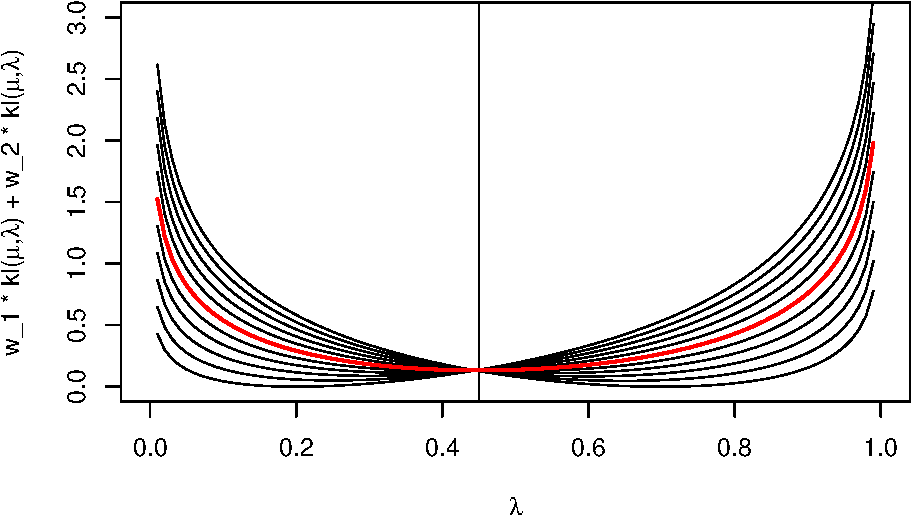
\includegraphics[width=0.8\linewidth]{Draft_files/figure-latex/unnamed-chunk-1-1} 

}

\caption{Budget allocation across arms for APT and SLR algorithms in simulation 2.}\label{fig:unnamed-chunk-1}
\end{figure}

\subsubsection{\texorpdfstring{Simulation 3: Bernoulli with
\(\tau = 0.01\)}{Simulation 3: Bernoulli with \textbackslash{}tau = 0.01}}\label{simulation-3-bernoulli-with-tau-0.01}

In the third experiment, we lower the threshold further to
\(\tau = 0.1\) and arrange the arms on a \(\log_{10}\) scale around it.
Again, there is no epsilon interval. We add one additional arm, thus now
classifying eleven arms. We run the same arms as previously. Notice that
the experiment horizon is now \(10000\) rounds instead of \(7000\)
rounds as in the previous experiment. We test the same algorithms used
in the previous two experiments.

\begin{longtable}[]{@{}rrrrrrrrrrr@{}}
\caption{Mean of arms in simulation 3 compared to a threshold of
0.01.}\tabularnewline
\toprule
V1 & V2 & V3 & V4 & V5 & V6 & V7 & V8 & V9 & V10 & V11\tabularnewline
\midrule
\endfirsthead
\toprule
V1 & V2 & V3 & V4 & V5 & V6 & V7 & V8 & V9 & V10 & V11\tabularnewline
\midrule
\endhead
1e-04 & 3e-04 & 6e-04 & 0.001 & 0.0018 & 0.0032 & 0.0056 & 0.0141 &
0.0178 & 0.0316 & 0.1\tabularnewline
\bottomrule
\end{longtable}

Looking at the performance after 7000 rounds, we see that the problem
appears to be slightly more difficult compared to the previous one. We
see that up until this point the variance-based strategies cannot
improve upon APT. Also, SLR has not yet crossed the 10\% empirical
error. We observe that in the following rounds EVT decreases at an
exponential rate and thus crosses the error of APT and continues to
improve. At the end of the budget, the improvement of SLR compared to
the other algorithms is again large, and likely to increase. However,
Bayes-UCB is again the best performing algorithm and is improving at a
faster rate than SLR. As in the previous experiment, Bayes-UCB and SLR
show significant improvements on this Bernoulli problem with very small
means and threshold compared to APT in particular.

\begin{figure}

{\centering \includegraphics[width=0.8\linewidth]{Draft_files/figure-latex/simulation3_results-1} 

}

\caption{Performance comparison of algorithms for simulation 3.}\label{fig:simulation3_results}
\end{figure}

\subsubsection{Simulations 4 and 5: Exponential and Poisson
Distributions}\label{simulations-4-and-5-exponential-and-poisson-distributions}

In \autoref{sec:LRforUnivariateExponentialFamily}, we show that the
likelihood ratio has a very useful form for the univariate exponential
family of distributions, which allows us to use the SLR algorithm not
only on Bernoulli arms, but also on Exponential or Poisson
distributions, for example. In simulation 4, we consider Exponential
distributions, in simulation 5, we test the algorithms on Poisson
distributions.

We run the same algorithms as before except for Bayes-UCB (even though
it should certainly be possible to adapt it to these case based on a
Gamma prior). In the case of the Exponential arms, we classify against
\(\tau = 1\) and have sampled their mean parameters of the arms from an
Exponential distribution with rate \(\theta = 1\). The Poisson arms are
classified against a threshold of \(\tau = 0.4\), with the mean
parameters being sampled from an Exponential distribution with mean
\(\mu = 0.7\). In both cases, we classify 20 arms.

For the Exponential arms, APT crosses the 0.1 error mark first, followed
by the AugUCB algorithm. All algorithms perform better than uniform
sampling. After more than half of the budget, the SLR algorithm jumps in
performance and performs better than APT and AugUCB. Indeed, the AugUCB
basically stops improving after half of the budget. This is a
consequence of it eliminating arms it believes to know very well. This
happens at an error rate of less than \(0.01\). On average, the AugUCB
samples only for 2564 rounds of the budget of 4000 rounds across the
5000 simulations.

The early elimination (when compared to the Bernoulli experiments) might
be caused by the fact that the AugUCB assumes the variance of the arms
to be in \([0,1]\), which does not hold for half of the arms in the
experiment. Similar goes for the EVT algorithm which is only able to
catch up at the very end of the budget.

\begin{figure}

{\centering \includegraphics[width=0.8\linewidth]{Draft_files/figure-latex/simulation4_results-1} 

}

\caption{Performance comparison of algorithms for simulation 4.}\label{fig:simulation4_results}
\end{figure}

In the case of Poisson arms, the performance of the arms is more clear
cut. As expected, SLR improves APT and the other strategies. APT
outperforms the EVT algorithm, which occurs even though the variance of
all arms considered in this experiment is in \([0,1]\). But similarly to
the Bernoulli simulations, the EVT might again have a hard time dealing
with sequences of observations that are all equal to \(0\) for a long
time. After about 1000 observations, APT and EVT appear to improve at
about the same rate, but APT had a much better initial exploration
phase.

\begin{figure}

{\centering \includegraphics[width=0.8\linewidth]{Draft_files/figure-latex/simulation5_results-1} 

}

\caption{Performance comparison of algorithms for simulation 5.}\label{fig:simulation5_results}
\end{figure}

\subsection{\texorpdfstring{Real Data
\label{sec:RealData}}{Real Data }}\label{real-data}

In the following, we present the results of two experiments performed on
a real world data set. While most new multi-armed bandit algorithms are
assessed on synthetic data, as we have done in
\autoref{sec:SyntheticData}, a real world data set is useful to observe
how algorithms perform in presence of, for example, not fully i.i.d.
samples. While of course every company tries to make their experiments
as ideal as possible, there will always be problems. Thus our
experiments serve as a first robustness check on the algorithms
introduced before.

\subsubsection{The Data Set}\label{the-data-set}

Data have been collected by the German online shop
\href{https://amorelie.de}{Amorelie} as part of standard website
analytics. For 197 selected products, we observe the number of users
visiting each product's detail page (PDP) at a given minute. The data
set we use here has been collected during the entire month of November
2016. It can be considered time series data collected at minutely
frequency. Thus the data contain 43200 observations per product, and
overall 8510400 observations.

Since we want to run an offline comparison of bandit algorithms, it is
important to have at each time point an observation for each arm. Given
that, it is easy to evaluate the perfomance of algorithms that make
different decisions at different point in times and thus do not observe
the same samples. By having an observation for each arm at any given
time point, each algorithm had at least the opportunity to observe a
certain sample. Other papers (for example, Li et al., 2011) have solved
this problem by using a sample drawn uniformly during, for example, an
A/B test. Then, if the next observation in the sample is not from the
same arm that the algorithm would like to draw from, observations are
discarded until the next observation from the selected arm.

The choice of using what is basically multiple time series data as the
sample offers a simple way of running the algorithms just as often on
the data as for simulated data. The goal is to perform 5000 runs over
the sample to confidently assess the performance. Since we want to
preserve the potential time dependency of the data, a simple resampling
of the data is not an option to create the needed 5000 variations of the
sample. Instead we perform time series cross validation. To preserve the
autocorrelation, one can create different samples of \(X\) observations
by sliding a window of size \(X\) over the time series. Moving the
window one period (in our case one minute) at a time, one ensures that
no sample shares start and end observation with another sample. In
particular, this means for a given bandit strategy and two samples that
the observations that the algorithm collects as feedback during the
initialization phases differ from sample to sample and are never the
same. This is because during initialization every strategy pulls arms
\(1, ..., K\) (or \(1,...,2K\) for EVT) once in this order.

While the data is count data (the number of visits to a PDP during a
given minute), we binarize the data by applying a certain threshold. If
the count is above this threshold, the new observation is \(1\), else
\(0\). Thus we have a binary time series of length 43200 for each of the
197 products. Given that the number of visitors that come to a given PDP
is likely to vary by time of day and by day, and in general over time,
we expect that the mean of the time series to not be stable over time.
For example, less visitors will come during night than during the
evening. This leads to a decrease in the average, and a daily
seasonality. On the other hand, more users may visit the site during a
weekend, thus leading to a spike on Saturdays and Sundays. Because of
the latter time dependency, it is best practice to run online A/B tests
for at least a week, or an integer multiple of weeks, so as to take into
account the weekly seasonality in the time series. For this reason, the
experiments we present below were run on \(60 \cdot 24 \cdot 7 = 10080\)
observations for each arm, so as to have a sample for one full week.

We can look at summary statistics for the sample means of the 197
products over the month of November to get a first impression of the
data we are dealing with. We see that most products have a small mean,
which is very common also for actual conversion rate or click-through
rate data that can be tested with A/B tests or multi-armed bandits. Yet
the sample of products contains a few outliers with very large view
rates, with a maximum rate of 78\%. If we used a threshold \(\gamma\) to
binarize the count data, then this means that on average every fourth
minute the count of visitors was below \(\gamma\) for this product. On
the other hand, we conclude that using thresholding bandit strategies to
test the products against a threshold of for example
\(\tau = \frac{2}{60} = 0.333\) or \(\tau = \frac{5}{60} = 0.083\) is
likely to create more complex problems than a threshold of, say,
\(\tau = \frac{15}{60} = 0.25\) would.

\begin{longtable}[]{@{}rrrrrr@{}}
\caption{Summary Statistics for View Rates of 197
Products}\tabularnewline
\toprule
Mean & Minimum & 25\% Quantile & Median & 75\% Quantile &
Maximum\tabularnewline
\midrule
\endfirsthead
\toprule
Mean & Minimum & 25\% Quantile & Median & 75\% Quantile &
Maximum\tabularnewline
\midrule
\endhead
0.12 & 0 & 0.036 & 0.074 & 0.136 & 0.778\tabularnewline
\bottomrule
\end{longtable}

\subsubsection{Experiment 1}\label{experiment-1}

In the first experiment, we pick ten arms randomly from the set of 197
arms. The experiment is run with a budget of \(T=10080\) samples during
each of the \(5000\) iterations for which we repeat the experiment.
Given the time series cross-validation idea described above, this means
that in total, \(15080\) observations of the \(43200\) available
observations per arm are used in training. In the thresholding bandit
problem, we classify arms as below or above a threshold. Thus we can
evaluate the strategies also based on whether their classifications are
correct in a holdout sample. As this holdout sample, we can use the
10080 observations in our data set that follow the first 15080
observations used in training. In the table below, we present the count
rates of the ten products for both training and test samples.

\begin{longtable}[]{@{}lrrrrrrrrrr@{}}
\caption{Count rates for ten products for both training and test
sample.}\tabularnewline
\toprule
& V1 & V159 & V64 & V139 & V189 & V70 & V114 & V148 & V118 &
V119\tabularnewline
\midrule
\endfirsthead
\toprule
& V1 & V159 & V64 & V139 & V189 & V70 & V114 & V148 & V118 &
V119\tabularnewline
\midrule
\endhead
Training & 0.001 & 0.013 & 0.027 & 0.053 & 0.059 & 0.071 & 0.071 & 0.102
& 0.156 & 0.158\tabularnewline
Test & 0.000 & 0.011 & 0.022 & 0.055 & 0.058 & 0.064 & 0.060 & 0.115 &
0.150 & 0.130\tabularnewline
\bottomrule
\end{longtable}

We see that while the rates do vary across training and test samples,
they are relatively stable which is likely due to the fact that the
samples come from an entire week's worth of observations. In particular,
since we test against a threshold of \(\tau = \frac{2}{60} = 0.333\) in
this experiment, the classifications of arms do not differ across
training and test data. A correct classification after training will be
correct in the test set. For the rest of the analysis, we thus evaluate
the performance using the training rates.

When comparing the rates against the threshold, we see that three
products are below the already small threshold. Product \(V64\) seems to
be especially difficult to classify correctly, even without time
dependency. On the other hand, arms \(V119\) and \(V118\) should be much
easier than the rest.

In order to visualize the time dependency that we expect for our
samples, we plot a moving average of the mean of the time series for the
first week of data. To remove the daily seasonality, we select a moving
average window of \(60\cdot24 = 1440\) observations. To make the time
dependency even more obvious, we contrast the actual data against
synthetic data generated using the sample means of the actual data.

The graph again underlines that arm \(V64\) is likely to be very
difficult to classify given that it's moving average even crosses the
threshold twice. The same is true for arm \(V139\), which is not visible
when considering the overall mean alone. Furthermore, arms \(V159\) and
\(V189\) come very close to the threshold at times.

\begin{figure}

{\centering 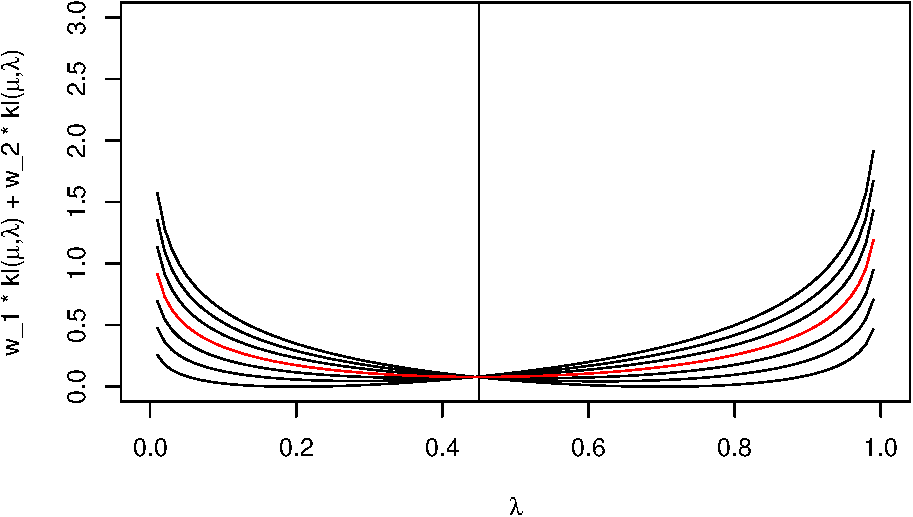
\includegraphics[width=0.8\linewidth]{Draft_files/figure-latex/unnamed-chunk-2-1} 

}

\caption{Rolling average for the arms used in experiment 1.}\label{fig:unnamed-chunk-2}
\end{figure}

These difficulties seem to have a large impact on the performance of all
algorithms. Given that the data are \(\{0,1\}\) observations, we can
compare all algorithms in a setting in which one expects all assumptions
to hold before having observed the data. The distribution is
sub-Gaussian for the APT algorithm, bounded between \(0\) and \(1\) for
the variance-based algorithms, and assumed to be Bernoulli for the SLR
algorithm. Additionally, we use the Bayes-UCB algorithm as it performed
best on the synthetic data.

We set \(\epsilon = 0\), and \(\tau = 2/60\). For the AugUCB algorithm
we use the parameters as in Mukherjee et al. (2017), that is,
\(\rho = 1/3\). For B-UCB we set the prior to \(\alpha_0 = \tau\) and
\(\beta_0 = 1-\tau\), and pick \(c=1\). All other algorithms are
parameter free.

\begin{figure}

{\centering \includegraphics[width=0.8\linewidth]{Draft_files/figure-latex/unnamed-chunk-3-1} 

}

\caption{Performance comparison of algorithms for experiment 1.}\label{fig:unnamed-chunk-3}
\end{figure}

Compared to the previous simulations with synthetic data, the results
are dramatically poor. First of all, we see that all strategies perform
poorly. All of them end above the 10\% error rate mark after 1 week of
data. Second, the uniform sampling strategy fares best when evaluated
against the sample mean of all observations used during training. This
of course is the opposite of what we would like to see, and the opposite
of what we saw on the synthetic data, where we were able to improve upon
the naive strategy. Third, again in contrast to the results on synthetic
data, we observe non-monotonicity in the error curves. Given that the
highs and lows run very much parallel for the different models, it
stands to reason that this effect is caused by the variation in means of
the arms over time. Indeed, roughly comparing the error curves to the
moving averages in the previous figure, the increase in errors after
round \(5000\) and the decreasing error after round \(7500\) seems to
line up with the fluctuations observed in the data. Given that we
evaluate the models against a sample mean of all observations, it is not
surprising that the uniform sampling strategy has a certain advantage
when it comes to ``factoring out'' the seasonalities. In contrast, the
adaptive sampling schemes try to adapt more or less quickly to the
changes in the means; a feature that would be valuable in a cumulative
regret multi-armed bandit setting. Here, however, it leads to wrong
estimates of the overall sample mean.

If we focus on a comparison of adaptive sampling strategies and less on
their globally bad performance, we see that the variance based
strategies perform worse than APT and SLR. Very dramatic is the behavior
of the Augmented-UCB algorithm, which first seems to perform well; this,
however, is a result of it mostly pulling arms uniformly, until it
starts to adapt its sampling and discarding arms after nearly 5000
rounds. The result is a dramatic increase in error which leads to the
worst performance at the budget horizon. The difference between APT,
SLR, and EVT is small, and their performance fluctuates in sync. None of
them is really able to converge due to the changes in the underlying
means. Advantageous only seems to be the fact that their behavior is
less erratic than that of the AugUCB strategy given that they do not
discard arms.

\subsubsection{Experiment 2}\label{experiment-2}

In order to underline the results of the previous experiment, we perform
a second experiment using the data collected by Amorelie. We increase
the threshold to \(\tau = \frac{5}{60} = 0.833\) to make the problem in
general slightly easier, and again pick 10 arms at random from the data
set of 197 arms. We again use a sliding window of \(10080\) observations
to create \(5000\) iterations and look at the training and test sample
means as in the previous experiment.

Some arms, in particular \(V110\) and \(V150\), but also \(V103\),
\(V149\), \(V104\), and \(V112\) are quite close to the threshold. Two
arms, \(V129\) and \(V32\) appear to have basically no positive
observation in the training set. On the other hand, arm \(V154\) is
larger than the threshold by a fair amount and should be easier to
classify.

\begin{longtable}[]{@{}lrrrrrrrrrr@{}}
\caption{Count rates for ten products for both training and test
sample.}\tabularnewline
\toprule
& V112 & V129 & V104 & V76 & V103 & V110 & V150 & V149 & V32 &
V154\tabularnewline
\midrule
\endfirsthead
\toprule
& V112 & V129 & V104 & V76 & V103 & V110 & V150 & V149 & V32 &
V154\tabularnewline
\midrule
\endhead
Training & 0.000 & 0 & 0.012 & 0.044 & 0.049 & 0.053 & 0.055 & 0.095 &
0.123 & 0.199\tabularnewline
Test & 0.013 & 0 & 0.011 & 0.040 & 0.049 & 0.063 & 0.060 & 0.114 & 0.137
& 0.202\tabularnewline
\bottomrule
\end{longtable}

As in the previous experiment, we can also take a look at the one day
moving averages of the arms to quickly assess the time dependency of the
means. Given that the data here are collected at the same time points as
the data used in the previous experiment, it is not surprising to see a
similar spike in means during the second half of the observations with
the maximum moving average around index 7500. We also observe that these
fluctuations are heavier for products with in general larger means (that
is, more visitors on the website). But these fluctuations are clearly
much larger and systematic than those observed for synthetic data with
the same sample means.

Given the moving averages and the previous experiment, the performance
results of Experiment 2 shown in the next figure are not surprising. We
recognize the same structure as previously. The uniform sampling
strategy performs the best. The adaptive sampling strategies perform
bad, do not converge, and end above the 10\% error rate mark. This time,
AugUCB is not (yet) the worst performing strategy, but equally erratic
after it eventually adapts its sampling. This time around, it even has
two spikes in its adaptive phase. Again, APT, SLR, and EVT perform in
sync and more or less equally bad, with EVT slightly better than APT and
SLR this time around. Interestingly, Bayes-UCB performs clearly worst of
all strategies. Its performance changes at the same time as
Augmented-UCB starts to adapt its sampling strategy, near round 7000.

This last fact is of particular interest, as Bayes-UCB is dramatically
better than the other strategies in experiments on synthetic data. On
the right hand side of the same figure, the performance of the
algorithms on synthetic data from Bernoulli distributions with the same
sample mean is depicted. On this data, Bayes-UCB performs very well,
ending at an average error of about 0.1\% of the simulations. This
mirrors its performance observed in the previous simulations with
synthetic data. Also all other adaptive strategies perform clearly
better now, and their error rates are strictly decreasing.
Interestingly, the uniform sampling scheme is now much worse than in the
experiment on real data; it does no longer have the advantage of
sampling the different mean phases at a representative rate. Excluding
Bayes-UCB, we see that the SLR algorithm performs the best, followed by
the variance-based algorithms. APT comes in at the same error rate as
uniform sampling. While the difference between SLR and EVT are less than
2\% (1.2\% vs 3\%), the difference to uniform sampling (10\%) is
relevant. The performance of 10\% error rate is achieved by SLR about
1000 observations earlier than by EVT.

\begin{figure}

{\centering \includegraphics[width=0.8\linewidth]{Draft_files/figure-latex/unnamed-chunk-4-1} 

}

\caption{Rolling average of arms used in experiment 2.}\label{fig:unnamed-chunk-4}
\end{figure}

\begin{figure}

{\centering \includegraphics[width=0.8\linewidth]{Draft_files/figure-latex/unnamed-chunk-8-1} 

}

\caption{Performance results of algorithms in experiment 2.}\label{fig:unnamed-chunk-8}
\end{figure}

Again using a plot of the pulls at each round across the 5000
simulations in Figure 17, we can try to understand why some strategies
perform well on synthetic data, but poorly on the time series data.

We observe that the patterns across algorithms are quite similar, while
the patterns are very different across data sets. On the synthetic data,
given that arm \(V149\) is clearly the most difficult arm to classify
due to its closeness to the threshold \(\tau\), all algorithms focus a
major share of their budget on this arm. The speed at which they start
to do so, however, differs. Perhaps surprisingly, the best performing
Bayes-UCB algorithm increases its focus on arm \(V149\) the slowest,
while in many iterations spending budget on exploring other arms. This
is surprising as the Bayes-UCB algorithm's exploration factor was
originally conceived for the cumulative regret problem. Thus one would
expect it to explore \emph{less} than other algorithms. But its
performance does not seem to be easily explained by the lessened focus
on the most difficult arm; else we would expect the APT algorithm to
perform second best. However, both SLR and EVT perform better than APT
while converging more quickly to a higher share of samples allocated to
the most difficult arm.

Something that might be hidden by this aggregated view of all 5000
iterations are a share of iterations in which the EVT completely fails
by exploring wrong arms for long periods. This effect might even be more
drastic for the APT algorithm. Even though it seems as if its behavior
is very similar to SLR and EVT, the overall performance is not better
than the performance of uniform sampling. Taking this reasoning into
account, one can hypothesize that the Bayes-UCB algorithm finds the most
difficult arm uniformly across most iterations as the rounds increase,
while other algorithms either find the most difficult arm right away or
never and thus have many iterations that end with a misclassification.

For the real data, the difference between Bayes-UCB and the other
algorithms is just as apparent. As is the effect of the time varying
means of the arms on the rate at which they are sampled. APT, SLR, and
EVT all focus quickly in many iterations on the still most difficult arm
\(V149\). However, in the case of the real data this behavior is not
rewarded in the end, as this leads to biased samples and thus wrong
estimation of the overall sample mean against which the algorithms are
evaluated. We see in the curves of arms \(V32\) and arm \(V154\) that
the EVT algorithm is less impacted by daily seasonalities, while APT
clearly is.

\begin{figure}

{\centering \includegraphics[width=0.8\linewidth]{Draft_files/figure-latex/unnamed-chunk-9-1} 

}

\caption{Budget allocation of algorithms across arms on real and synthetic data in experiment 2.}\label{fig:unnamed-chunk-9}
\end{figure}

\subsubsection{Experiments Conclusion}\label{experiments-conclusion}

In the two previous experiments, we observe that the real time series
data poses a major hurdle for the adaptive sampling algorithms. It seems
that the poor performance can be mostly explained by the seasonality and
sudden changes in the samples over time. The observations clearly are
not i.i.d. sampled. However, the effect might be overly stark due to the
fact that we use minutely time series data, which leads to observations
even when in minutes when there are few or no users (during night). In
contrast, the daily seasonality might be less represented in an actual
online experiment observations are only drawn when there is an actual
visitor on the site (and a proper conversion rate would fluctuate less
than the count of visitors on a given product page).

Furthermore, some of the problems in dealing with the fluctuating
distributions might be specific to the thresholding bandit problem as
opposed to the cumulative regret or best-arm identification problems. In
the experiments above, we observe that the order of the arms is mostly
unaffected by the seasonalities and fluctuations, which would mean that
the best arm could still be identified. In contrast, given that all arms
are individually classified against the \emph{fixed} threshold, a weekly
seasonality can declare a correct classification on the first half of
the sample null and void on the second half of the sample.

\section{Conclusion}\label{conclusion}

\section{Notes}\label{notes}

The author thanks Alexandra Carpentier, Andrea Locatelli, and Urun Dogan
for many hours of valuable feedback and ideas.

\section{References}\label{references}

\section{Appendix}\label{appendix}

\subsection{\texorpdfstring{Proof of Thresholding Bandit Lower Bound
\label{sec:AppendixAPTLB}}{Proof of Thresholding Bandit Lower Bound }}\label{proof-of-thresholding-bandit-lower-bound}

We now give a proof for the lower bound for the thresholding bandit
problem stated in \autoref{theorem:Locatelli2016Theorem1}.

\emph{Proof of Theorem \ref{theorem:Locatelli2016Theorem1}}: Locatelli
et al. (2016) derive a lower bound for the thresholding bandit problem.
We restate the proof here. The idea is as follows. The problem
formulation considered in the paper describes bandit problems for
\(R\)-sub-Gaussian distributions. To show a lower bound, we show that
every algorithm is expected to make a certain error even if we consider
a very restricted scenario. Even then, the best algorithm will have a
maximum error probability with which it cannot distinguish between the
actual setting and slightly changed settings (under which the answer for
the true setting leads to a misclassification).

Consider the thresholding bandit setting as in \autoref{sec:Setup}. More
specifically, consider a problem in which all arms follow Normal
distributions \(\nu_i\) with mean \(\mu_i\) and variance
\(\sigma^2 = 1\). ``in which w''e set \(\tau = 0\) and \(\epsilon = 0\)
w.l.o.g. Consequently, for each arm \(i\) the distance from the
threshold is given by \(\Delta_i = |\mu_i - \tau| + \epsilon = \mu_i\).
Thus, we have for every arm the distribution
\(\nu_i = \mathcal{N}(\mu_i,1) = \mathcal{N}(\Delta_i,1)\). Furthermore,
define for each arm \(i \in \{1, \dots, K\}\) the alternative
distribution \(\nu_i' = \mathcal{N}(-\Delta_i,1)\). It is easy to see
that this is equivalent to a ``flip around the threshold''. Arms that
originally have a mean larger than the threshold have a mean smaller
than the threshold after the flip.

The intuition now is that every arm \(i \in \{1,\dots,K\}\) generates a
sample for every time point \(t\in \{1, \dots, T\}\) from its
distribution \(\nu_i\) before the algorithm starts to choose arms. Thus,
we have a \(T \times K\) table of realized observations from the product
distribution given by
\(\mathcal{B}^0 = \nu_1^0 \otimes \ldots \otimes \nu_K^0 = \nu_1^0 \otimes \ldots \otimes \nu_K\).
This is a product distribution where the \(K\) different means are all
above the threshold. We would hope that an algorithm classifies the
means accordingly. However, we will show in what follows that any
algorithm makes a certain error by not being able to distinguish
\(\mathcal{B}^0\) from at least one of \(K\) alternative product
distributions \(\mathcal{B}^i, i \in \{1, \dots, K\}\), of which each
differs only slightly in one arm from the original distribution, and has
the same overall complexity (as defined by
\(H = \sum_{i=1}^K (\Delta_i)^{-2}\)). We require \(K\) different
distributions so that an algorithm sampling arm \(i\) very often for
some reason will not have a smaller lower bound by chance.

For each of the \(K\) arms, we introduce an alternative model of the
following kind. Before the start of the algorithm, we introduce a slight
variation in the setup. The idea is similar to how one can switch arms
in the pure exploration setup for multi-armed bandits (compare Audibert
et al., 2010; Garivier \& Kaufmann, 2016) to ``confuse'' any algorithm
without introducing additional complexity to the specified problem.
However, since we do not compare arms directly with each other in the
thresholding bandit problem (switching arms would still keep all means
above the threshold), we instead need to flip an arm \(i\) with respect
to the threshold in order to get the alternative model
\(\mathcal{B}_i\). Since the threshold is \(\tau = 0\), we have for the
flipped arm the new distribution \(\nu_i'\) as defined above. Indeed,
define the new product distribution
\(B^i = \nu_1^i \otimes \dots \otimes \nu_K^i\) where for
\(k \leq K, \nu_k' := \nu_i \mathbbm{1}_{k \neq i} + \nu_i' \mathbbm{1}_{k=i}\).
This arm flip corresponds to multiplying all \(X_{i,t}\) of arm \(i\) by
\(-1\).

As in Locatelli et al. (2016), let for \(i \leq K\),
\(\mathbb{P}_{\mathcal{B}^i}\) be the probability distribution
describing all samples that a bandit strategy can potentially collect up
to horizon \(T\), i.e.~according to the samples
\((X_{k,s})_{k\leq K, s \leq T} \sim (\mathcal{B}^i)^{\otimes T}\).
\((T_k)_{k\leq K}\) denotes the number of samples collected on arm \(k\)
until time \(T\).

At this point, we have defined a finite set of problems of Gaussian
distributions with fixed variance 1 for a given set of set of gaps
between the means of the distributions and the threshold,
\((\Delta_k)_k\). We now proof a lower bound on the worst case regret of
any algorithm; that is, the maximum error probability that even the best
algorithm makes on this problem.

\subsubsection{Statistical Decision}\label{statistical-decision}

The expected loss in our thresholding bandit setting,
\(\mathbb{E}[\mathcal{L}(T)]\), corresponds directly to the probability
of making a wrong classification of any of the \(K\) means. In general,
given a binary decision function \(g\), define events
\(\Omega = \{g = 0\}\) and \(\Omega^C = \{g = 1\}\). Assume that the
decision \(g\) distinguishes between two states of the world, \(H_0\)
and \(H_1\). Then an overall error probability can be seperated into
\(P_{H_0}(g=1) + P_{H_1}(g = 0) = P_{H_0}(\Omega^C) + P_{H_1}(\Omega)\).

In our case, \(H_0\) may correspond to the state in which we have
\(\mathcal{B}^0\), and \(H_1\) corresponds to the case where any arm has
been flipped, \(\mathcal{B}^i\). Furthermore, we consider the events in
which the algorithm classifies arm \(i\) as being above the threshold:
\(\mathcal{A}_i = \{i \in \hat{S}_\tau\}\). The event on which all arms
are being classified as above the threshold is consequently given by
\(\mathcal{A} = \bigcap_{i=1}^K \mathcal{A}_i\). We could thus separate
the error probability \(\mathbb{E}[\mathcal{L}(T)]\) into
\(\mathbb{P}_{\mathcal{B}^i}(\mathcal{A}_i)\) and
\(\mathbb{P}_{\mathcal{B}^0}(\mathcal{A}^C)\). However, Theorem 1 does
not bound the overall regret, but the maximum error probability on the
\(K+1\) different models. We can write this now as

\begin{align}
\max_{i \in \{0, \dots, K\}} \mathbb{E}_{\mathcal{B}^i} (\mathcal{L}(T)) & \geq \max \big( \max_{i \in \{1, \dots, K\}} \mathbb{P}_{\mathcal{B}^i}(\mathcal{A}_i), \mathbb{P}_{\mathcal{B}^0}(\mathcal{A}^C) \big) \\
& = \max \big( \max_{i \in \{1, \dots, K\}} \mathbb{P}_{\mathcal{B}^i}(\mathcal{A}_i), 1 - \mathbb{P}_{\mathcal{B}^0}(\mathcal{A}) \big) \label{LocatelliTheorem1ExpRegret}
\end{align}

\subsubsection{Empirical Kullback-Leibler
Divergence}\label{empirical-kullback-leibler-divergence}

In order to give a bound on the previous equation, we start by
considering \(\mathbb{P}_{\mathcal{B}^i}(\mathcal{A}_i)\). This
probability can be written as the expected change in the likelihood of
observed data when moving from distribution \(P_{\mathcal{B}_0}\) to
\(P_{\mathcal{B}_i}\), times the probability under the original state.
In other words, the probability of event \(\mathcal{A}_i\) under state
\(\mathcal{B}^i\) is given as the probability of \(\mathcal{A}_i\) under
the (original) state \(\mathcal{B}^0\) multiplied by a factor. This
factor describes whether the new distribution increases or decreases the
probability of the event, and is given by the change in the data
likelihoods due to moving from \(\mathcal{B}^0\) to \(\mathcal{B}^i\),
expressed as the expected likelihood ratio under \(\mathcal{B}^0\). By
definition, the latter is equal to the empirical Kullback-Leibler
divergence of the two distributions.

We will define the change of distribution in terms of the empirical
log-likelihood for our case. Then, we will show how to replace the
log-likelihood by the empirical Kullback-Leibler divergence. Let us
first introduce the empirical Kullback-Leibler divergence.

Let every \(\nu_i, \nu_i'\) be dominated by the Lebesgue measure
\(\lambda\). Then their density functions are given by
\(f_i = \frac{\der \nu_i}{\der \lambda}\) and
\(f_i' = \frac{\der \nu_i'}{\der \lambda}\) respectively. For
\(T \geq t \geq 0\), define the empirical Kullback-Leibler divergence
for an i.i.d. sample \(X_{k,1}, \dots,X_{k,t}\) as

\begin{align*}
\hat{\KL}_{k,t} & = \frac{1}{t} \sum_{s=1}^{t} \log(\frac{\der \nu_k'}{\der \nu_k}(X_{k,s})) \\
& = \frac{1}{t} \sum_{s=1}^{t} \log \big(\frac{f_k'(X_{k,s})}{f_k(X_{k,s})} \big) \\
& = \frac{1}{t} \log \big( \prod_{s=1}^{t} \frac{f_k'(X_{k,s})}{f_k(X_{k,s})} \big) \\
& \stackrel{\text{iid}}{=} \frac{1}{t} \log \big( \frac{f_k'(X_{k,1}, \dots,X_{k,t})}{f_k(X_{k,1}, \dots,X_{k,t})} \big) \\
& = \frac{1}{t} \log \big( \text{LR}((X_{k,1}, \dots,X_{k,t}), \nu_k', \nu_k) \big),
\end{align*}

where \(\text{LR}((X_{k,1}, \dots,X_{k,t}), \nu_k', \nu_k)\) is the
likelihood ratio for the sample.

Since we consider Gaussian distributions with variance \(\sigma^2 = 1\),
we have density functions
\(f_i(x) \propto \exp \big(-\frac{1}{2} (x-\Delta_i)^2\big)\) and
\(f_i'(x) \propto \exp \big(-\frac{1}{2} (x+\Delta_i)^2\big)\). Plugging
this into the above definition of the empirical Kullback-Leibler
divergence, we easily see

\begin{align*}
\hat{\KL}_{k,t} & = \frac{1}{t} \sum_{s=1}^{t} \log \Big(\frac{\exp \big(-\frac{1}{2} (X_{k,s}+\Delta_k)^2\big)}{\exp \big(-\frac{1}{2} (X_{k,s}-\Delta_k)^2\big)} \Big) \\
& = \frac{1}{t} \sum_{s=1}^{t} \log \Big( \exp \big(-\frac{1}{2} (X_{k,s}+\Delta_k)^2 + \frac{1}{2} (X_{k,s}-\Delta_k)^2 \big) \Big) \\
& = - \frac{1}{t} \sum_{s=1}^{t} 2 X_{k,s} \Delta_k
\end{align*}

\subsubsection{Change of Distribution}\label{change-of-distribution}

We are now ready to state the change of distribution. As alluded to
above, we consider how the probability changes for the event
\(\mathcal{A}_i\) when we move from \(\mathcal{B}^0\) to
\(\mathcal{B}^i\). When flipping arm \(i\), we only change the samples
of this arm, that is, the first \(T_i\) observations that the algorithm
draws from arm \(i\). The change of distribution is then defined as:

\begin{align*}
\mathbb{P}_{\mathcal{B}^i}(\mathcal{A}_i) & = \mathbb{E}_{\mathcal{B}^0} \big[\mathbbm{1}_{\mathcal{A}_i} \text{LR}((X_{i,1}, \dots,X_{i,T_i}), \nu_i', \nu_i) ] \\
& = \mathbb{E}_{\mathcal{B}^0} \big[\mathbbm{1}_{\mathcal{A}_i} \exp (- T_i \hat{\KL}_{i,T_i}) ]
\end{align*}

Obviously, \(\hat{\KL}_{i,T_i}\) depends on the realized samples
\(X_{i,1}, \dots,X_{i,T_i}\). Consequently, we need to find a bound on
\(\hat{\KL}_{i,T_i}\) itself to incorporate the uncertainty involved in
this metric.

\subsubsection{Concentration of the Empirical Kullback-Leibler
Divergence}\label{concentration-of-the-empirical-kullback-leibler-divergence}

For our problem, the Kullback-Leibler divergence of \(\nu_k'\) from
\(\nu_k\) is given by \(\KL_k := \KL(\nu_k', \nu_k) = 2\Delta_k^2\), and
consequently

\begin{equation*}
|\hat{\KL}_{k,t} - \KL_{k,t}| = |-\frac{2}{t} \Delta_k \sum_{s=1}^{t}(X_{k,s} - \Delta_k)|
\end{equation*}

itself is a normally distributed random variable with mean zero and a
variance decreasing in \(t\). Thus, one can show as in Locatelli et al.
(2016) that \(\mathbb{P}_{\mathcal{B}^i}(\xi) \geq 3/4\) for the event

\begin{equation}
\xi = \{ \forall k \leq K, \forall t \leq T, |\hat{\KL}_{k,t} - \KL_{k,t}| \leq 4 \Delta_k \sqrt{\frac{\log(4(\log(T)+1)K)}{t}}\}. \label{LocatelliTheorem1EventXi}
\end{equation}

Thus, in order to bound the empirical Kullback-Leibler divergence in our
change of measure, we can consider the intersection of \(\mathcal{A}_i\)
and \(\xi\) as follows and plug in the bound on event \(\xi\):

\begin{align*}
\mathbb{P}_{\mathcal{B}^i}(\mathcal{A}_i) & = \mathbb{E}_{\mathcal{B}^0} \big[\mathbbm{1}_{\mathcal{A}_i} \exp (- T_i \hat{\KL}_{i,T_i}) ] \\
& \geq \mathbb{E}_{\mathcal{B}^0} \big[\mathbbm{1}_{\mathcal{A}_i \cap \xi} \exp (- T_i \hat{\KL}_{i,T_i}) ] \\
& \geq \mathbb{E}_{\mathcal{B}^0} \big[\mathbbm{1}_{\mathcal{A}_i \cap \xi} \exp (- 2 \Delta_i^2 T_i - 4 \Delta_i \sqrt{T_i} \sqrt{\log(4(\log(T)+1)K)}) ]
\end{align*}

Two things are left to do: With \(T_i\), we still have one random
variable left which we cannot leave in our bound. Second, we are
actually not interested in \(\mathbb{P}_{\mathcal{B}^i}(\mathcal{A}_i)\)
but in
\(\max_{i \in \{1,\dots,K\}} \mathbb{P}_{\mathcal{B}^i}(\mathcal{A}_i)\).

\subsubsection{\texorpdfstring{Bounding \(T_i\) for
\(\max_{i \in \{1,\dots,K\}}\mathbb{P}_{\mathcal{B}^i}(\mathcal{A}_i)\)}{Bounding T\_i for \textbackslash{}max\_\{i \textbackslash{}in \textbackslash{}\{1,\textbackslash{}dots,K\textbackslash{}\}\}\textbackslash{}mathbb\{P\}\_\{\textbackslash{}mathcal\{B\}\^{}i\}(\textbackslash{}mathcal\{A\}\_i)}}\label{bounding-t_i-for-max_i-in-1dotskmathbbp_mathcalbimathcala_i}

We are actually interested in bounding
\(\max_{i \in \{1,\dots,K\}} \mathbb{P}_{\mathcal{B}^i}(\mathcal{A}_i)\).
In general it holds that
\(\max_{1 \leq i \leq K} (X_1, \dots, X_K) \geq \frac{1}{K}\sum_{i=1}^K X_i\).
Thus we can write:

\begin{align*}
\max_{i \in \{1,\dots,K\}} \mathbb{P}_{\mathcal{B}^i}(\mathcal{A}_i) & \geq \frac{1}{K} \sum_{i=1}^{K} \mathbb{P}_{\mathcal{B}^i}(\mathcal{A}_i) \\
& \geq \frac{1}{K} \sum_{i=1}^{K} \mathbb{P}_{\mathcal{B}^i}(\mathcal{A}_i \cap \xi) \\
& \geq \frac{1}{K} \sum_{i=1}^{K} \mathbb{E}_{\mathcal{B}^0} \big[\mathbbm{1}_{\mathcal{A}_i \cap \xi} \exp (- 2 \Delta_i^2 T_i - 4 \Delta_i \sqrt{T_i} \sqrt{\log(4(\log(T)+1)K)}) ]
\end{align*}

where the second line is again the intersection of \(\mathcal{A}_i\) and
\(\xi\) as before, such that we can apply the change of distribution in
the third line.

What is left to show is a bound on \(T_i\). Given that we want to show
that even the best algorithm makes an error on at least one of the
problems (one of the arms), it makes sense to show that \(T_i\) is upper
bounded. This implies that no arm can be infinitely sampled; we cannot
reach full confidence in any arm, and a residual error probability
should remain.

First, let \(a = \Delta_i \sqrt{T_i}\) and
\(b = 4\sqrt{\log((4\log(T)+1)K)}\). Then use \(ab \leq a^2 + b^2\) to
write \(ab \leq \Delta_i^2 T_i + 16\log((4\log(T)+1)K)\). And so:

\begin{align*}
\max_{i \in \{1,\dots,K\}} \mathbb{P}_{\mathcal{B}^i}(\mathcal{A}_i) & \geq \frac{1}{K} \sum_{i=1}^{K} \mathbb{E}_{\mathcal{B}^0} \big[\mathbbm{1}_{\mathcal{A}_i \cap \xi} \exp (- 3 \Delta_i^2 T_i - 16 \log(4(\log(T)+1)K)) ]
\end{align*}

Furthermore, we know that the sum of the individual arm pulls has to be
equal to the overall number of pulls (equal to the budget in the fixed
budget sense), \(\sum_i T_i = T\), and furthermore we know that
\(T_i>0\). The latter holds since any reasonable algorithm has to check
each arm at least once in our setup. Thus it is easy to show that
\(\exists i: T_i \leq \frac{T}{H \Delta_i^2} = \frac{T}{(\sum_{i=1}^{K} \Delta_i^{-2}) \Delta_i^2}\).
To see this, assume the opposite:
\(\forall i: T_i > T \frac{\sum_{i=1}^K \Delta_i^2}{\Delta_i^2}\). This
implies however
\(\sum_{i=1}^K T_i > \sum_{i=1}^K T \frac{\sum_{i=1}^K \Delta_i^2}{\Delta_i^2} = T \cdot 1 = T\)
which is a contradiction.

So we can write \((\Delta_i \sqrt{T_i})^2 \leq \frac{T}{H}\). We use
\(\mathcal{A} = \cap_{i=1}^K \mathcal{A}_i\) to write:

\begin{align*}
\max_{i \in \{1,\dots,K\}} \mathbb{P}_{\mathcal{B}^i}(\mathcal{A}_i) & \geq \frac{1}{K} \sum_{i=1}^{K} \mathbb{E}_{\mathcal{B}^0} \big[\mathbbm{1}_{\mathcal{A}_i \cap \xi} \exp (- 3 \Delta_i^2 T_i - 16 \log(4(\log(T)+1)K)) \big] \\
& = \mathbb{E}_{\mathcal{B}^0} \big[\mathbbm{1}_{\mathcal{A} \cap \xi} \frac{1}{K} \sum_{i=1}^{K} \exp (- 3 \Delta_i^2 T_i - 16 \log(4(\log(T)+1)K)) \big]
\end{align*}

We write
\(\frac{1}{K} \sum_{i=1}^K \exp(-3T_i \Delta_i^2) \geq \frac{1}{K} \sum_{i=1}^K \exp(-3 T/H) = \exp(-3 T/H)\).
Thus:

\begin{align*}
\max_{i \in \{1,\dots,K\}} \mathbb{P}_{\mathcal{B}^i}(\mathcal{A}_i) & = \mathbb{E}_{\mathcal{B}^0} \Big[\mathbbm{1}_{\mathcal{A} \cap \xi} \frac{1}{K} \sum_{i=1}^{K} \exp (- 3 \Delta_i^2 T_i) \exp \big(-16 \log(4(\log(T)+1)K)\big) \Big] \\
& \geq \mathbb{E}_{\mathcal{B}^0} \Big[\mathbbm{1}_{\mathcal{A} \cap \xi} \frac{1}{K} \sum_{i=1}^{K} \exp \big(- 3 \frac{T}{H}\big) \exp \big(-16 \log(4(\log(T)+1)K)\big) \Big] \\
& = \mathbb{E}_{\mathcal{B}^0} \Big[\mathbbm{1}_{\mathcal{A} \cap \xi} \exp \big(- 3 \frac{T}{H}\big) \exp \big(-16 \log(4(\log(T)+1)K)\big) \Big] \\
& = \mathbb{P}_{\mathcal{B}^0} (\mathcal{A} \cap \xi) \exp \Big(- 3 \frac{T}{H} -16 \log \big(4(\log(T)+1)K\big)\Big)
\end{align*}

\subsubsection{Bringing everything
together}\label{bringing-everything-together}

Consider again the risk which we need to bound from equation
\eqref{LocatelliTheorem1ExpRegret}. We bound the maximum expected loss
over all \(\mathcal{B}_i\). By using again the fact that in general
\(\max_{1 \leq i \leq K} (X_1, \dots, X_K) \geq \frac{1}{K} \sum_{i = 1}^K X_i\),
we plug into our previous calculations:

\begin{align}
\max_{i \in \{0, \dots, K\}} \mathbb{E}_{\mathcal{B}^i} (\mathcal{L}(T)) & \geq \max \big( \max_{i \in \{1, \dots, K\}} \mathbb{P}_{\mathcal{B}^i}(\mathcal{A}_i), 1 - \mathbb{P}_{\mathcal{B}^0}(\mathcal{A}) \big) \\
& \geq \frac{1}{2}\mathbb{P}_{\mathcal{B}^0} (\mathcal{A} \cap \xi) \exp \Big(- 3 \frac{T}{H} -16 \log \big(4(\log(T)+1)K\big)\Big) + \frac{1}{2}(1 - \mathbb{P}_{\mathcal{B}^0}(\mathcal{A})) \label{LocatelliTheorem1DefinitionOfRisk}
\end{align}

From \eqref{LocatelliTheorem1EventXi} we know that for any
\(i \in \{0, \dots, K\}\), \(\mathbb{P}_{\mathcal{B}^i}(\xi) \geq 3/4\).
Following the argument in Locatelli et al. (2016), we now consider two
cases: \(\mathbb{P}_{\mathcal{B}^0}(\mathcal{A}) \geq 1/2\) and
\(\mathbb{P}_{\mathcal{B}^0}(\mathcal{A}) \leq 1/2\). In the former
case, we can plug in the two probabilities into
\eqref{LocatelliTheorem1DefinitionOfRisk}. If
\(\mathbb{P}_{\mathcal{B}^0}(\mathcal{A}) \geq 1/2\) and
\(\mathbb{P}_{\mathcal{B}^0}(\xi) \geq 3/4\), then
\(\mathbb{P}_{\mathcal{B}^0}(\mathcal{A} \cap \xi) \geq 1/4\). Thus:

\begin{align*}
\max_{i \in \{0, \dots, K\}} \mathbb{E}_{\mathcal{B}^i} (\mathcal{L}(T)) & \geq \max \big( \max_{i \in \{1, \dots, K\}} \mathbb{P}_{\mathcal{B}^i}(\mathcal{A}_i), 1 - \mathbb{P}_{\mathcal{B}^0}(\mathcal{A}) \big) \\
& \geq \frac{1}{2}\mathbb{P}_{\mathcal{B}^0} (\mathcal{A} \cap \xi) \exp (- 3 \frac{T}{H} -16 \log(4(\log(T)+1)K)) + \frac{1}{2}(1 - \mathbb{P}_{\mathcal{B}^0}(\mathcal{A})) \\
& \geq \frac{1}{8} \exp (- 3 \frac{T}{H} -16 \log(4(\log(T)+1)K))
\end{align*}

where we drop the second summand of the second line so that the
inequality holds.

On the other hand, when
\(\mathbb{P}_{\mathcal{B}^0}(\mathcal{A}) \leq 1/2\), then we know that
\(\mathbb{P}_{\mathcal{B}^0}(\mathcal{A} \cap \xi) \leq 1/2\) for any
\(\mathbb{P}_{\mathcal{B}^0}(\xi)\). At the same time
\(1-\mathbb{P}_{\mathcal{B}^0}(\mathcal{A}) = \mathbb{P}_{\mathcal{B}^0}(\mathcal{A^C}) \geq 1/2\).
Consequently,
\(1/4 \leq \frac{1}{2}(1 - \mathbb{P}_{\mathcal{B}^0}(\mathcal{A})) \leq 1/2\),
while
\(\frac{1}{2}\mathbb{P}_{\mathcal{B}^0} (\mathcal{A} \cap \xi) \exp (- 3 \frac{T}{H} -16 \log(4(\log(T)+1)K)) \geq 0\).
And so the stronger lower bound in that case is, as noticed by Locatelli
et al. (2016), given simply by

\begin{align*}
\max_{i \in \{0, \dots, K\}} \mathbb{E}_{\mathcal{B}^i} (\mathcal{L}(T)) & \geq \max \big( \max_{i \in \{1, \dots, K\}} \mathbb{P}_{\mathcal{B}^i}(\mathcal{A}_i), 1 - \mathbb{P}_{\mathcal{B}^0}(\mathcal{A}) \big) \\
& \geq 1 - \mathbb{P}_{\mathcal{B}^0}(\mathcal{A}) = \mathbb{P}_{\mathcal{B}^0}(\mathcal{A^C}) \\
& \geq \frac{1}{2}
\end{align*}

\subsection{\texorpdfstring{Lower Bound on Probability of Error in
FB-Top-\(m\) with Gaussian Arms
\label{sec:KaufmannLBTopMGaussian}}{Lower Bound on Probability of Error in FB-Top-m with Gaussian Arms }}\label{lower-bound-on-probability-of-error-in-fb-top-m-with-gaussian-arms}

While we would like to move beyond Gaussian distributions in the work at
hand, the idea for the proof might show a way of how the ideas can be
transferred to the thresholding bandit problem. We first state the
result and then discuss the proof.

\begin{lemma}[Lemma 15, Kaufmann et al., 2016] \label{theorem:KaufmannEtAlLemma15}
Let $\nu$ and $\nu'$ be two bandit models such that $S^*_m(\nu) \neq S^*_m(\nu')$. Then

\begin{equation*}
\max \big( \mathbb{P}_{\nu}(S \neq S^*_m(\nu)), \mathbb{P}_{\nu'}(S \neq S^*_m(\nu')) \big) \geq \frac{1}{4} \exp \Big(-\sum_{a=1}^{K} \mathbb{E}_{\nu}[N_a] \KL(\nu_a, \nu_a') \Big).
\end{equation*}
\end{lemma}

The following theorem only holds in the case of Gaussian bandit models
with equal known variance.

\begin{theorem}[Theorem 17, Kaufmann et al., 2016] \label{theorem:KaufmannEtAlTheorem17}

Let $\mathcal{M}_m = \{\nu = (\nu_1, \dots, \nu_K): \nu_a = \mathcal{N}(\mu_a, \sigma^2), \mu_a \in \mathbb{R}, \mu_{[m]}\neq \mu_{[m+1]}\}.$ Furthermore, let $\nu$ be such that $\mu_1 > \dots > \mu_m > \mu_{m+1} > \dots > \mu_K$, and let

\begin{equation*}
H^+(\nu) = \sum_{a=1}^m \frac{2\sigma^2}{(\mu_a - \mu_{m+1})^2}, \quad H^-(\nu) = \sum_{a=m+1}^K \frac{2\sigma^2}{(\mu_m - \mu_a)^2} \quad
and \quad
H(\nu) = H^+(\nu) + H^-(\nu).
\end{equation*}

There exists $a \in \{1, \dots, m\}$ and $b \in \{m+1, \dots, K\}$ such that the bandit model $\nu^{[a,b]}$ described in Figure 4 (Kaufmann et al., 2016) satisfies $H(\nu^{[a,b]}) < H(\nu)$ and is such that

\begin{equation*}
\max \big( p_t(\nu),p_t(\nu^{[a,b]})\big) \geq \frac{1}{4} \exp \big(-\frac{4t}{\bar{H}(\nu)}\big), \quad where \quad \bar{H}(\nu) = \frac{H(\nu) \min(H^+(\nu),H^-(\nu))}{H(\nu)+\min(H^+(\nu),H^-(\nu))}
\end{equation*}
\end{theorem}

Given that we are again in the Top-\(m\) setting, the proof idea is
similar to the proof of Theorem \ref{theorem:KaufmannEtAlTheorem4} in
that we again consider problems in which we switch arms around the
threshold implied by \(\mu_{[m]}\) and \(\mu_{[m+1]}\). Given that, one
might hope to apply a similar proof to the thresholding bandit problem.
As we see in \autoref{sec:AppendixAPTLB}, a flip around the threshold is
used in the proof of the lower bound in Theorem 1 of Locatelli et al.
(2016). However, there, again, the distributions are assumed to be
Gaussian. This brings the big advantage that the Kullback-Leibler
divergence is symmetric, and the feedback can take values on all
\(\mathbb{R}\). This is important, as is allows us to easily define
alternative problems by a flip around the threshold with the same
complexity as the original problem. This would not hold for
KL-divergences that are not symmetric (e.g., for Bernoulli arms). For
the full proof, refer to page 20 in Kaufmann et al. (2016).

\subsection{Proof of Corollary 1}\label{proof-of-corollary-1}

\textbf{Proof}: The proof follows closely the proof of Theorem 12 in
Kaufmann et al. (2016) and is again an application of their
transportation Lemma, Lemma 2.

Consider the one-armed bandit problem, \(K = 1\) with the canonical
exponential family of distributions distribution \(\nu_1\) parameterized
by its mean \(\mu_1\). Furthermore, given we are in the thresholding
bandit problem, we have a threshold \(\tau\) against which the arm is
classified. Assume w.l.o.g. that for \(\nu_1\), \(\mu_1 \geq \tau\).
Thus, \(\mathcal{S}_{\tau}^* = \{1\}\). After \(T\) rounds, a consistent
algorithm returns with error probability \(p_T(\nu)\) the guess
\(\hat{\mathcal{S}}_{\tau}\). Thus, we have for the event
\(A = (\hat{\mathcal{S}}_\tau = \{1\})\) the probability
\(\mathbb{P}_{\nu}(A)\). On the other hand, define the alternative model
\(\nu'\) with mean \(\mu_1' < \tau\) such that the correct
classification from \(\nu\) is now wrong:
\(\mathcal{S}_{\tau}^* {'} = (\mathcal{S}_{\tau}^*)^C = \{\emptyset\}\).
Consequently, since the algorithm is still consistent on this problem,
we have that \(\mathbb{P}_{\nu'}(A) = p_t(\nu')\). Thus, we expect that
as we let \(t\) increase, \(\mathbb{P}_{\nu'}(A)\) will decrease while
\(\mathbb{P}_{\nu}(A)\) will increase.

Indeed, given we consider only consistent algorithms, there should exist
a number of samples for which the probability of the correct decision in
problem \(\nu\) is larger than the error probability in problem
\(\nu'\), that is: for every \(\epsilon > 0\), there exists
\(t_0(\epsilon)\) such that for all \(t \geq t_0(\epsilon)\) we have

\begin{equation}
\mathbb{P}_{\nu'}(A) \leq \epsilon \leq \mathbb{P}_{\nu}(A). \label{eq:BoundForCorollary}
\end{equation}

Now, consider again Lemma 2 in Kaufmann et al. (2016). If we let the
algorithm be such that \(T = t\), we can apply the Lemma to the stopping
time \(\sigma = t\) a.s. and the event \(A\) to get

\[
\mathbb{E}_{\nu'}[N_1(t)]\KL(\nu_1', \nu_1) \geq d(\mathbb{P}_{\nu'}(A), \mathbb{P}_{\nu}(A)).
\]

We can lower bound the RHS by using the bound on
\(\mathbb{P}_{\nu'}(A)\) given in \eqref{eq:BoundForCorollary} and the
monotonicity of the binary relative entropy. We get:

\begin{align*}
\mathbb{E}_{\nu'}[N_1(t)]\KL(\nu_1', \nu_1) & = t \KL(\nu_1', \nu_1) \\
& \geq d(\mathbb{P}_{\nu'}(A), \mathbb{P}_{\nu}(A)) \\
& \geq d(\epsilon, 1- p_t(\nu)) \\
& = \epsilon \log\Big(\frac{\epsilon}{1-p_t(\nu)}\Big) + (1-\epsilon) \log \Big(\frac{1-\epsilon}{p_t(\nu)}\Big) \\
& \geq (1-\epsilon) \log \Big(\frac{1-\epsilon}{p_t(\nu)}\Big) + \epsilon \log(\epsilon) \\
\end{align*}

Letting \(\epsilon \rightarrow 0\), we get

\[
t \KL(\nu_1', \nu_1) \geq \log \Big(\frac{1}{p_t(\nu)}\Big) = -\log p_t(\nu).
\] To make the bound as tight as possible, we choose the alternative
model that minimizes \(\KL(\nu_1', \nu_1)\) while still ensuring that
\(\mathcal{S}_{\tau}^* {'} = \{\emptyset\}\). In our case of the
thresholding bandit with univariate exponential family distributions,
this is given by choosing \(\mu_1' = \tau\). By pluggin in, we get the
result:

\[
t \KL(\tau, \mu_1) \geq -\log p_t(\nu).
\]

\subsection{\texorpdfstring{Bayes-UCB Algorithm for the Thresholding
Bandit Problem
\label{sec:AppendixBUCB}}{Bayes-UCB Algorithm for the Thresholding Bandit Problem }}\label{bayes-ucb-algorithm-for-the-thresholding-bandit-problem}

We show how the Bayes-UCB algorithm (Algorithm 1, Kaufmann et al., 2012)
is adopted to the thresholding bandit problem to be used in the
experiments in chapter \autoref{chap:Experiments}.

We adopt their Algorithm 1 for Bernoulli distributions as follows:

\IncMargin{1em}

\begin{algorithm}
\SetKwInOut{Input}{Input}\SetKwInOut{Output}{Output}
\Input{\emph{$\tau$, $\epsilon$, $T$, $\Pi^0$ (initial prior on $\mu$), $c$ (parameters of the quantile)}}
\Output{$\hat{S}_\tau = \{i \in \mathbb{A},  \hat{\mu}_i(T) \geq \tau\}$}
\BlankLine
\emph{Pull each arm once}\;
\For{$t = K+1$ \KwTo $T$}{
\For{$i = 1$ \KwTo $K$}{
  \emph{Compute $q_i(t) = Q\Big(1-\frac{1}{t(\log T)^c}, \lambda_i^{t-1}\Big)$}\;
  \emph{Compute $B_i(t) = $}\;
  \If{$\hat{\sigma}^2_{i}(t) = 0$}{\emph{Set $\hat{\sigma}^2_{i}(t) = 1/T$}}
}
  \emph{Pull arm $I_t = \arg \min_{i\leq K} B_i^{SLR_{2D}}(t)$ as in \autoref{eqn:SLR2DIndex}}\;
  \emph{Observe reward $X \sim \nu_{I_t}$}\;
}
\caption{2D-SLR algorithm for Normal distributions with unknown mean and unknown variance}\label{algo_slr_2d}
\end{algorithm}

\DecMargin{1em}

\subsection{Empirical Analysis of the Bayes-UCB Algorithm in Simulation
2}\label{empirical-analysis-of-the-bayes-ucb-algorithm-in-simulation-2}

In order to assess the excellent performance of the Bayes-UCB algorithm,
which comes at a surprise given that is is designed for the cumulative
regret setting and thus should tend to explore the arms to less, we also
plot the budget allocation of three different Bayes-UCB versions. The
three versions differ in the quantile parameter \(c\) (compare
\autoref{sec:AppendixBUCB}) for which we set here
\(c \in \{1/5, 1, 5\}\) to explore more or less. In Kaufmann et al.
(2012), the cumulative regret upper bound for the Bayes-UCB is shown for
\(c\geq 5\), though they report that the choice of \(c=0\) worked much
better in their experiments. In our problem, it makes also sense that
the versions with smaller quantiles (smaller \(c\)) tend to perform
better than

\begin{figure}

{\centering \includegraphics[width=0.8\linewidth]{Draft_files/figure-latex/simulation2_results_bucb-1} 

}

\caption{Performance comparison of algorithms for simulation 2.}\label{fig:simulation2_results_bucb}
\end{figure}

\begin{figure}

{\centering \includegraphics[width=0.8\linewidth]{Draft_files/figure-latex/unnamed-chunk-10-1} 

}

\caption{Budget allocation for the Bayes-UCB algorithm in simulation 2 at three different values for the quantile parameter c.}\label{fig:unnamed-chunk-10}
\end{figure}

\subsection{Empirical Comparison of APT, SLR, and Bayes-UCB in
Experiment
2}\label{empirical-comparison-of-apt-slr-and-bayes-ucb-in-experiment-2}

\begin{figure}

{\centering \includegraphics[width=0.8\linewidth]{Draft_files/figure-latex/unnamed-chunk-11-1} 

}

\caption{Budget allocation for the Bayes-UCB algorithm in simulation 2 at three different values for the quantile parameter c.}\label{fig:unnamed-chunk-11}
\end{figure}

\begin{figure}

{\centering \includegraphics[width=0.8\linewidth]{Draft_files/figure-latex/unnamed-chunk-12-1} 

}

\caption{Budget allocation for the Bayes-UCB algorithm in simulation 2 at three different values for the quantile parameter c.}\label{fig:unnamed-chunk-12}
\end{figure}


\end{document}
